% Options for packages loaded elsewhere
\PassOptionsToPackage{unicode}{hyperref}
\PassOptionsToPackage{hyphens}{url}
%
\documentclass[
  letterpaper,
]{book}

\usepackage{amsmath,amssymb}
\usepackage{lmodern}
\usepackage{iftex}
\ifPDFTeX
  \usepackage[T1]{fontenc}
  \usepackage[utf8]{inputenc}
  \usepackage{textcomp} % provide euro and other symbols
\else % if luatex or xetex
  \usepackage{unicode-math}
  \defaultfontfeatures{Scale=MatchLowercase}
  \defaultfontfeatures[\rmfamily]{Ligatures=TeX,Scale=1}
\fi
% Use upquote if available, for straight quotes in verbatim environments
\IfFileExists{upquote.sty}{\usepackage{upquote}}{}
\IfFileExists{microtype.sty}{% use microtype if available
  \usepackage[]{microtype}
  \UseMicrotypeSet[protrusion]{basicmath} % disable protrusion for tt fonts
}{}
\makeatletter
\@ifundefined{KOMAClassName}{% if non-KOMA class
  \IfFileExists{parskip.sty}{%
    \usepackage{parskip}
  }{% else
    \setlength{\parindent}{0pt}
    \setlength{\parskip}{6pt plus 2pt minus 1pt}}
}{% if KOMA class
  \KOMAoptions{parskip=half}}
\makeatother
\usepackage{xcolor}
\setlength{\emergencystretch}{3em} % prevent overfull lines
\setcounter{secnumdepth}{5}
% Make \paragraph and \subparagraph free-standing
\ifx\paragraph\undefined\else
  \let\oldparagraph\paragraph
  \renewcommand{\paragraph}[1]{\oldparagraph{#1}\mbox{}}
\fi
\ifx\subparagraph\undefined\else
  \let\oldsubparagraph\subparagraph
  \renewcommand{\subparagraph}[1]{\oldsubparagraph{#1}\mbox{}}
\fi

\usepackage{color}
\usepackage{fancyvrb}
\newcommand{\VerbBar}{|}
\newcommand{\VERB}{\Verb[commandchars=\\\{\}]}
\DefineVerbatimEnvironment{Highlighting}{Verbatim}{commandchars=\\\{\}}
% Add ',fontsize=\small' for more characters per line
\usepackage{framed}
\definecolor{shadecolor}{RGB}{241,243,245}
\newenvironment{Shaded}{\begin{snugshade}}{\end{snugshade}}
\newcommand{\AlertTok}[1]{\textcolor[rgb]{0.68,0.00,0.00}{#1}}
\newcommand{\AnnotationTok}[1]{\textcolor[rgb]{0.37,0.37,0.37}{#1}}
\newcommand{\AttributeTok}[1]{\textcolor[rgb]{0.40,0.45,0.13}{#1}}
\newcommand{\BaseNTok}[1]{\textcolor[rgb]{0.68,0.00,0.00}{#1}}
\newcommand{\BuiltInTok}[1]{\textcolor[rgb]{0.00,0.23,0.31}{#1}}
\newcommand{\CharTok}[1]{\textcolor[rgb]{0.13,0.47,0.30}{#1}}
\newcommand{\CommentTok}[1]{\textcolor[rgb]{0.37,0.37,0.37}{#1}}
\newcommand{\CommentVarTok}[1]{\textcolor[rgb]{0.37,0.37,0.37}{\textit{#1}}}
\newcommand{\ConstantTok}[1]{\textcolor[rgb]{0.56,0.35,0.01}{#1}}
\newcommand{\ControlFlowTok}[1]{\textcolor[rgb]{0.00,0.23,0.31}{#1}}
\newcommand{\DataTypeTok}[1]{\textcolor[rgb]{0.68,0.00,0.00}{#1}}
\newcommand{\DecValTok}[1]{\textcolor[rgb]{0.68,0.00,0.00}{#1}}
\newcommand{\DocumentationTok}[1]{\textcolor[rgb]{0.37,0.37,0.37}{\textit{#1}}}
\newcommand{\ErrorTok}[1]{\textcolor[rgb]{0.68,0.00,0.00}{#1}}
\newcommand{\ExtensionTok}[1]{\textcolor[rgb]{0.00,0.23,0.31}{#1}}
\newcommand{\FloatTok}[1]{\textcolor[rgb]{0.68,0.00,0.00}{#1}}
\newcommand{\FunctionTok}[1]{\textcolor[rgb]{0.28,0.35,0.67}{#1}}
\newcommand{\ImportTok}[1]{\textcolor[rgb]{0.00,0.46,0.62}{#1}}
\newcommand{\InformationTok}[1]{\textcolor[rgb]{0.37,0.37,0.37}{#1}}
\newcommand{\KeywordTok}[1]{\textcolor[rgb]{0.00,0.23,0.31}{#1}}
\newcommand{\NormalTok}[1]{\textcolor[rgb]{0.00,0.23,0.31}{#1}}
\newcommand{\OperatorTok}[1]{\textcolor[rgb]{0.37,0.37,0.37}{#1}}
\newcommand{\OtherTok}[1]{\textcolor[rgb]{0.00,0.23,0.31}{#1}}
\newcommand{\PreprocessorTok}[1]{\textcolor[rgb]{0.68,0.00,0.00}{#1}}
\newcommand{\RegionMarkerTok}[1]{\textcolor[rgb]{0.00,0.23,0.31}{#1}}
\newcommand{\SpecialCharTok}[1]{\textcolor[rgb]{0.37,0.37,0.37}{#1}}
\newcommand{\SpecialStringTok}[1]{\textcolor[rgb]{0.13,0.47,0.30}{#1}}
\newcommand{\StringTok}[1]{\textcolor[rgb]{0.13,0.47,0.30}{#1}}
\newcommand{\VariableTok}[1]{\textcolor[rgb]{0.07,0.07,0.07}{#1}}
\newcommand{\VerbatimStringTok}[1]{\textcolor[rgb]{0.13,0.47,0.30}{#1}}
\newcommand{\WarningTok}[1]{\textcolor[rgb]{0.37,0.37,0.37}{\textit{#1}}}

\providecommand{\tightlist}{%
  \setlength{\itemsep}{0pt}\setlength{\parskip}{0pt}}\usepackage{longtable,booktabs,array}
\usepackage{calc} % for calculating minipage widths
% Correct order of tables after \paragraph or \subparagraph
\usepackage{etoolbox}
\makeatletter
\patchcmd\longtable{\par}{\if@noskipsec\mbox{}\fi\par}{}{}
\makeatother
% Allow footnotes in longtable head/foot
\IfFileExists{footnotehyper.sty}{\usepackage{footnotehyper}}{\usepackage{footnote}}
\makesavenoteenv{longtable}
\usepackage{graphicx}
\makeatletter
\def\maxwidth{\ifdim\Gin@nat@width>\linewidth\linewidth\else\Gin@nat@width\fi}
\def\maxheight{\ifdim\Gin@nat@height>\textheight\textheight\else\Gin@nat@height\fi}
\makeatother
% Scale images if necessary, so that they will not overflow the page
% margins by default, and it is still possible to overwrite the defaults
% using explicit options in \includegraphics[width, height, ...]{}
\setkeys{Gin}{width=\maxwidth,height=\maxheight,keepaspectratio}
% Set default figure placement to htbp
\makeatletter
\def\fps@figure{htbp}
\makeatother
\newlength{\cslhangindent}
\setlength{\cslhangindent}{1.5em}
\newlength{\csllabelwidth}
\setlength{\csllabelwidth}{3em}
\newlength{\cslentryspacingunit} % times entry-spacing
\setlength{\cslentryspacingunit}{\parskip}
\newenvironment{CSLReferences}[2] % #1 hanging-ident, #2 entry spacing
 {% don't indent paragraphs
  \setlength{\parindent}{0pt}
  % turn on hanging indent if param 1 is 1
  \ifodd #1
  \let\oldpar\par
  \def\par{\hangindent=\cslhangindent\oldpar}
  \fi
  % set entry spacing
  \setlength{\parskip}{#2\cslentryspacingunit}
 }%
 {}
\usepackage{calc}
\newcommand{\CSLBlock}[1]{#1\hfill\break}
\newcommand{\CSLLeftMargin}[1]{\parbox[t]{\csllabelwidth}{#1}}
\newcommand{\CSLRightInline}[1]{\parbox[t]{\linewidth - \csllabelwidth}{#1}\break}
\newcommand{\CSLIndent}[1]{\hspace{\cslhangindent}#1}

\usepackage{booktabs}
\usepackage{longtable}
\usepackage{array}
\usepackage{multirow}
\usepackage{wrapfig}
\usepackage{float}
\usepackage{colortbl}
\usepackage{pdflscape}
\usepackage{tabu}
\usepackage{threeparttable}
\usepackage{threeparttablex}
\usepackage[normalem]{ulem}
\usepackage{makecell}
\usepackage{xcolor}
\makeatletter
\@ifpackageloaded{tcolorbox}{}{\usepackage[many]{tcolorbox}}
\@ifpackageloaded{fontawesome5}{}{\usepackage{fontawesome5}}
\definecolor{quarto-callout-color}{HTML}{909090}
\definecolor{quarto-callout-note-color}{HTML}{0758E5}
\definecolor{quarto-callout-important-color}{HTML}{CC1914}
\definecolor{quarto-callout-warning-color}{HTML}{EB9113}
\definecolor{quarto-callout-tip-color}{HTML}{00A047}
\definecolor{quarto-callout-caution-color}{HTML}{FC5300}
\definecolor{quarto-callout-color-frame}{HTML}{acacac}
\definecolor{quarto-callout-note-color-frame}{HTML}{4582ec}
\definecolor{quarto-callout-important-color-frame}{HTML}{d9534f}
\definecolor{quarto-callout-warning-color-frame}{HTML}{f0ad4e}
\definecolor{quarto-callout-tip-color-frame}{HTML}{02b875}
\definecolor{quarto-callout-caution-color-frame}{HTML}{fd7e14}
\makeatother
\makeatletter
\makeatother
\makeatletter
\@ifpackageloaded{bookmark}{}{\usepackage{bookmark}}
\makeatother
\makeatletter
\@ifpackageloaded{caption}{}{\usepackage{caption}}
\AtBeginDocument{%
\ifdefined\contentsname
  \renewcommand*\contentsname{Table of contents}
\else
  \newcommand\contentsname{Table of contents}
\fi
\ifdefined\listfigurename
  \renewcommand*\listfigurename{List of Figures}
\else
  \newcommand\listfigurename{List of Figures}
\fi
\ifdefined\listtablename
  \renewcommand*\listtablename{List of Tables}
\else
  \newcommand\listtablename{List of Tables}
\fi
\ifdefined\figurename
  \renewcommand*\figurename{Figure}
\else
  \newcommand\figurename{Figure}
\fi
\ifdefined\tablename
  \renewcommand*\tablename{Table}
\else
  \newcommand\tablename{Table}
\fi
}
\@ifpackageloaded{float}{}{\usepackage{float}}
\floatstyle{ruled}
\@ifundefined{c@chapter}{\newfloat{codelisting}{h}{lop}}{\newfloat{codelisting}{h}{lop}[chapter]}
\floatname{codelisting}{Listing}
\newcommand*\listoflistings{\listof{codelisting}{List of Listings}}
\makeatother
\makeatletter
\@ifpackageloaded{caption}{}{\usepackage{caption}}
\@ifpackageloaded{subcaption}{}{\usepackage{subcaption}}
\makeatother
\makeatletter
\@ifpackageloaded{tcolorbox}{}{\usepackage[many]{tcolorbox}}
\makeatother
\makeatletter
\@ifundefined{shadecolor}{\definecolor{shadecolor}{rgb}{.97, .97, .97}}
\makeatother
\makeatletter
\@ifpackageloaded{sidenotes}{}{\usepackage{sidenotes}}
\@ifpackageloaded{marginnote}{}{\usepackage{marginnote}}
\makeatother
\makeatletter
\makeatother
\ifLuaTeX
  \usepackage{selnolig}  % disable illegal ligatures
\fi
\IfFileExists{bookmark.sty}{\usepackage{bookmark}}{\usepackage{hyperref}}
\IfFileExists{xurl.sty}{\usepackage{xurl}}{} % add URL line breaks if available
\urlstyle{same} % disable monospaced font for URLs
\hypersetup{
  pdftitle={Research Toolkit},
  pdfauthor={Nikita Tkachenko},
  hidelinks,
  pdfcreator={LaTeX via pandoc}}

\title{Research Toolkit}
\author{Nikita Tkachenko}
\date{3/14/23}

\begin{document}
\frontmatter
\maketitle
\ifdefined\Shaded\renewenvironment{Shaded}{\begin{tcolorbox}[borderline west={3pt}{0pt}{shadecolor}, enhanced, frame hidden, breakable, interior hidden, sharp corners, boxrule=0pt]}{\end{tcolorbox}}\fi

\renewcommand*\contentsname{Table of contents}
{
\setcounter{tocdepth}{2}
\tableofcontents
}
\mainmatter
\bookmarksetup{startatroot}

\hypertarget{preface}{%
\chapter*{Preface}\label{preface}}
\addcontentsline{toc}{chapter}{Preface}

\markboth{Preface}{Preface}

This is a Quarto book.

To learn more about Quarto books visit
\url{https://quarto.org/docs/books}.

\begin{Shaded}
\begin{Highlighting}[]
\DecValTok{1} \SpecialCharTok{+} \DecValTok{1}
\end{Highlighting}
\end{Shaded}

\begin{verbatim}
[1] 2
\end{verbatim}

\bookmarksetup{startatroot}

\hypertarget{introduction}{%
\chapter{Introduction}\label{introduction}}

This is a book created from markdown and executable code.

See Knuth
(1984)\marginpar{\begin{footnotesize}\leavevmode\vadjust pre{\protect\hypertarget{ref-knuth84}{}}%
Knuth, Donald E. 1984. {``Literate Programming.''} \emph{Comput. J.} 27
(2): 97--111. \url{https://doi.org/10.1093/comjnl/27.2.97}.\vspace{2mm}\par\end{footnotesize}}
for additional discussion of literate programming.

\begin{Shaded}
\begin{Highlighting}[]
\DecValTok{1} \SpecialCharTok{+} \DecValTok{1}
\end{Highlighting}
\end{Shaded}

\begin{verbatim}
[1] 2
\end{verbatim}

\bookmarksetup{startatroot}

\hypertarget{summary}{%
\chapter{Summary}\label{summary}}

In summary, this book has no content whatsoever.

\begin{Shaded}
\begin{Highlighting}[]
\DecValTok{1} \SpecialCharTok{+} \DecValTok{1}
\end{Highlighting}
\end{Shaded}

\begin{verbatim}
[1] 2
\end{verbatim}

\bookmarksetup{startatroot}

\hypertarget{set-up}{%
\chapter{Set up}\label{set-up}}

We will be using R and RStudio IDE to download, clean, explore, and
model our data. R language was developed by statisticians for
statisticians and had intuitive syntax and workflow for creating
readable and \textbf{reproducible} code.

\hypertarget{download-r}{%
\section{Download R}\label{download-r}}

R is maintained through \href{https://cran.r-project.org/}{The
Comprehensive R Archive Network}.

\hypertarget{for-macos}{%
\subsection{For macOS}\label{for-macos}}

\begin{enumerate}
\def\labelenumi{\arabic{enumi}.}
\tightlist
\item
  Go to \url{https://cran.r-project.org/}
\item
  Select ``Download R for macOS''
\item
  If you have Apple Silicon mac (M1,M2\ldots) download the latest
  version that has -arm64 in its name (R-4.2.2-arm64.pkg)
\item
  If you have Intel Max Download one without -arm64 (R-4.2.2.pkg)
\item
  Follow the steps from the installation wizzard
\item
  The installer lets you customize your installation, but the defaults
  will be suitable for most users
\item
  Your computer might ask for your password before installing new
  programs
\end{enumerate}

\hypertarget{for-windows}{%
\subsection{For Windows}\label{for-windows}}

\begin{enumerate}
\def\labelenumi{\arabic{enumi}.}
\tightlist
\item
  Go to \url{https://cran.r-project.org/}
\item
  Select ``Download R for Windows''
\item
  Click on ``base''
\item
  Click the first link at the top of the new page (Download R-4.2.2 for
  Windows)
\item
  ink downloads an installer program, which installs the most up-to-date
  version of R for Windows.
\item
  Follow the steps from the installation wizzard
\item
  The installer lets you customize your installation, but the defaults
  will be suitable for most users
\item
  You might need administration privileges to install new software on
  your machine
\end{enumerate}

\hypertarget{download-rstudio}{%
\section{Download RStudio}\label{download-rstudio}}

Rstudio is like a Microsoft Word for writing text, but instead of text
RStudio helps you write in R. RStudio is also free and easy to install!
Go to \href{https://posit.co/download/rstudio-desktop/}{RStudio
Website}, click on DOWNLOAD RSTUDIO or select your operation system
below, and follow the isntallation instructions.

\hypertarget{configure-rstudio}{%
\section{Configure RStudio}\label{configure-rstudio}}

First watch an introduction to RStudio:
\url{https://www.youtube.com/watch?v=FIrsOBy5k58} and introduction to
projects: \url{https://www.youtube.com/watch?v=MdTtTN8PUqU}

Now the most crucial part!!! Change the default theme of RStudio from
light to dark! To do this

\begin{enumerate}
\def\labelenumi{\arabic{enumi}.}
\tightlist
\item
  Go to the top panel
\item
  Select the Tools tab
\item
  Navigate to Global Options
\item
  Select Appearance
\item
  In Editor Theme, select ``Dracula''
\item
  Click Apply
\end{enumerate}

Now let's install a cooler font with ligatures! Install fira-code:
\url{https://github.com/tonsky/FiraCode/wiki/Installing}.
\textbf{Restart} RStudio for the font to load. Then go back to
Appearance, choose FiraCode, and hit apply.

\hypertarget{install-packages}{%
\section{Install Packages}\label{install-packages}}

An R package is a collection of useful functions, documentation, and
data sets that can be used in your own R code after it is loaded. These
packages typically focus on a specific task and make use of pre-written
routines for various data science tasks.

You can install packages with a single line of code:

\begin{verbatim}
install.packages("tidyverse")
\end{verbatim}

You can also install multiple packages at the same time using c():

\begin{verbatim}
install.packages(c("tidyverse","gapminder"))
\end{verbatim}

You can load packages using the library() function:

\begin{verbatim}
library("tidyverse")
\end{verbatim}

Run the following command to install packages we will use in class

\begin{verbatim}
install.packages(c("tidyverse", "janitor", "esquisse", "modelsummary", "styler"))
\end{verbatim}

\part{Writing and Lit Review}

\hypertarget{write}{%
\chapter{Write}\label{write}}

WYSIWYG (What You See Is What You Get) editors are programs that allow
you to make and edit content visually without having to know how to
code. This means that you can see how your content will look as you're
creating it. They're very helpful for people who don't have experience
with coding or markup languages. Examples of WYSIWYG editors that you
may already be familiar with include Google Docs and Microsoft Word.
Learning how to use these tools is important because they are some of
the most widely used ones, and they teach you valuable skills like
formatting and writing. Plus, after using them for a while, you'll start
to appreciate the simplicity and efficiency of markup languages.

I strongly recommend that you develop expertise in these tools, as the
skills you acquire are highly transferable to other similar editors.
Additionally, it's a valuable investment as your colleagues are likely
to use them as well. To get started, I suggest checking out the MOS
Certification Series on LinkedIn Learning. These tutorials are designed
for those preparing to take MOS exams and cover a broad range of
functionality in Word, Excel, and PowerPoint. Even if you don't plan on
taking the exams, I highly encourage you to watch the tutorials. They're
a great resource for building your skills and improving your proficiency
in these essential tools!

\href{https://www.linkedin.com/learning-login/share?account=2204681\&forceAccount=false\&redirect=https\%3A\%2F\%2Fwww.linkedin.com\%2Flearning\%2Fcert-prep-word-associate-microsoft-office-specialist-for-office-2019\%3Ftrk\%3Dshare_ent_url\%26shareId\%3DSTM\%252FLOpvQwOb0jWc9D\%252FabQ\%253D\%253D}{here
is the link}

\hypertarget{markup-languages}{%
\section{Markup Languages}\label{markup-languages}}

Markup languages are sets of codes that provide structure and formatting
to documents, such as web pages, eBooks, and scientific papers. Unlike
WYSIWYG editors, which allow users to create content visually, markup
languages require the use of specific tags or codes to indicate how the
content should be displayed. These tags define the document structure,
formatting, and other attributes. Some of the most commonly used markup
languages include HTML, LaTeX, and Markdown. By learning a markup
language, you can have greater control over the appearance and
functionality of your digital documents. Additionally, markup languages
can help you focus more on writing letting templates handle all the
formatting. I promise after you switch there is no coming back! Your
assignments and web pages will look beautiful every time.

\hypertarget{html}{%
\subsection{HTML}\label{html}}

When you hear markup language you might think of Hypertext Markup
Language (HTML), which is used everywhere on the web to build up
structure and content. HTML uses tags to describe how to display content
in a browser. For instance, \textless br\textgreater{} will create a
line break, \textless img\textgreater{} will add an image and so on.
HTML is an essential component of web development, and learning how to
use HTML is the first step towards customizing your own web pages and
web applications. It is also often used in manipulating text in your
graphs.

\hypertarget{latex}{%
\subsection{LaTeX}\label{latex}}

Have you ever wondered why academic papers look so beautiful or why
every textbook looks the same? They are all written in LaTeX, a
typesetting system used for academic and scientific publishing. It is a
markup language that enables precise formatting of complex technical
documents. It is also famous for beautiful mathematical equations. With
LaTeX, users can create professional-looking documents with a high
degree of customization and flexibility. It is easy to pick up, but hard
to master. You can find many introductory tutorials online. Also,
ChatGPT does a great job at helping with LaTeX questions. If you have an
equation you want to transfer into LaTeX go to
\href{https://mathpix.com/image-to-latex}{MathPix}. It lets you convert
picture or screenshot into code.

Now you need to find an editor! The default is to use the online editor
\href{https://www.overleaf.com/}{Over Leaf}. You can start writing
without much headache, perfect! And if you have any question refer to
their extensive collection of guides.

\hypertarget{markdown}{%
\subsection{Markdown}\label{markdown}}

Markdown is perfect down the last-minute details. It was created as a
lightweight markup language for creating formatted text using a
plain-text editor. It appeals to human readers in its source code form
as a response to the complexity and inefficiency of existing markup
languages like HTML.

Markdown is popular among developers, writers, and bloggers due to its
simplicity and flexibility. It can also include links, images, and other
multimedia elements. Markdown is widely supported and can be used with a
variety of tools and platforms, including text editors, note-taking
apps, and content management systems. By learning Markdown, you can
create well-formatted and easy-to-read content quickly and efficiently
without the need for complex formatting tools or specialized software.
This book is written entirely in Markdown!

You can write markdown in almost any text editor. Nonetheless, I
recommend MacDown for Mac and Markdown Pad for Windows, or if you are
willing to pay, try Typora.

\hypertarget{yet-another-markup-language-yaml}{%
\subsection{Yet Another Markup Language
(YAML)}\label{yet-another-markup-language-yaml}}

YAML (Yet Another Markup Language) is a human-readable data
serialization language often used for configuration files and data
exchange. It uses indentation, key-value pairs, and directories and
supports different data types. Directories are used to organize data as
key-value pairs with indentation to indicate hierarchy. The key
represents a unique identifier or name, and the value represents
associated data or content. YAML is easy to read and write and is
popular in web development and software configuration. In YAML,

\begin{Shaded}
\begin{Highlighting}[]
\FunctionTok{book}\KeywordTok{:}
\AttributeTok{  }\FunctionTok{title}\KeywordTok{:}\AttributeTok{ }\StringTok{"Dead Souls"}
\AttributeTok{  }\FunctionTok{author}\KeywordTok{:}\AttributeTok{ }\StringTok{"Nikolai Gogol"}
\AttributeTok{  }\FunctionTok{date}\KeywordTok{:}\AttributeTok{ today}
\AttributeTok{  }\FunctionTok{chapters}\KeywordTok{:}
\AttributeTok{    }\KeywordTok{{-}}\AttributeTok{ index.qmd}
\AttributeTok{    }\KeywordTok{{-}}\AttributeTok{ chapter1.qmd}
\AttributeTok{  }\FunctionTok{appendix}\KeywordTok{:}
\AttributeTok{    }\KeywordTok{{-}}\AttributeTok{ appendix1.qmd}
\end{Highlighting}
\end{Shaded}

\begin{Shaded}
\begin{Highlighting}[]
\PreprocessorTok{\% Key value pairs}
\FunctionTok{title}\KeywordTok{:}\AttributeTok{ }\StringTok{"Dead Souls"}
\FunctionTok{author}\KeywordTok{:}\AttributeTok{ }\StringTok{"Nikolai Gogol"}
\FunctionTok{date}\KeywordTok{:}\AttributeTok{ today}

\PreprocessorTok{\% Directory/Map  }
\FunctionTok{chapters}\KeywordTok{:}
\AttributeTok{  }\KeywordTok{{-}}\AttributeTok{ index.qmd}
\AttributeTok{  }\KeywordTok{{-}}\AttributeTok{ chapter1.qmd}
\end{Highlighting}
\end{Shaded}

\hypertarget{pandoc}{%
\subsection{Pandoc}\label{pandoc}}

Pandoc (all documents) converts files from one markup format into
another. It supports a wide range of formats, including HTML, Markdown,
LaTeX, PDF, and Microsoft Word. With Pandoc, users can convert documents
from one markup language to another quickly and easily, without having
to edit or reformat the content manually.

Pandoc can be used for a variety of purposes, such as converting a
Markdown file to HTML for a web page, or converting a LaTeX document to
PDF for printing. It can also be used to merge multiple documents into a
single file, or to extract content from a document in a specific format.

Pandoc is highly customizable, with many options and settings available
for controlling the output format and appearance of the converted
document. It is widely used in academic and scientific publishing, as
well as in web development and documentation. By using Pandoc, users can
save time and effort by automating the conversion process between
different markup formats.

Pandoc is a command-line tool, but it can be integrated into some
markdown editors. It extends the capabilities of markdown by adding
support for tables, footnotes, citations, and more. For example, this
book was written in markdown and converted into HTML and PDF using
Pandoc.

\hypertarget{quarto}{%
\section{Quarto}\label{quarto}}

At this point, you might be wondering, ``why did I have to read about
these technologies?'' Because the combination of LaTeX, Markdown,
Pandoc, and YAML provides a powerful and flexible set for the creation
of documents. Those familiar with Sweave, Rmarkdown, and Jupyter
Notebooks will find Quarto to be a similar tool. Quarto builds upon the
success of Rmarkdown and Jupyter Notebooks, combining the best features
of Markdown with new functionality and eliminating the need for
additional packages. It provides attractive default formatting options
and easy customization. If you have experience writing in Markdown,
Quarto will be a breeze to use.

What can it do?

\begin{itemize}
\tightlist
\item
  Create Reproducible Documents and Reports.
\item
  Create Dynamic Content with Python, R, Julia, and Observable.
\item
  Create professional-grade content, including articles, reports,
  presentations, websites, blogs, and books, in a variety of formats
  such as HTML, PDF, MS Word, ePub, and more.
\item
  Author with scientific markdown, including equations, citations,
  crossrefs, figure panels, callouts, advanced layout, and more.
\item
  Create interactive tutorials and notebooks.
\end{itemize}

\hypertarget{installing}{%
\subsection{Installing}\label{installing}}

To use quarto you don't need any special software, if you would like you
can use even use a text editor to create your .qmd files and command
line to render the document. However, working in IDE will make your life
much easier. I prefer to use RStudio, after all, Quarto is a product of
Posit (former RStudio), but it Visual Studio Code also works great. If
you have not installed RStudio nor Visual Studio Code yet follow INSERT
CHAPTER LINK.

\hypertarget{rstudio}{%
\subsubsection{RStudio}\label{rstudio}}

From within Rstudio you can install quarto as you install any other
package. Additionally, you should install TinyTeX, a minimal set of
packages required to compile LaTeX documents. You can both by running
the following command in R.

\begin{Shaded}
\begin{Highlighting}[]
\NormalTok{install.packages(c("quarto", "tinytex"))}
\end{Highlighting}
\end{Shaded}

\hypertarget{visual-studio-code}{%
\subsubsection{Visual Studio Code}\label{visual-studio-code}}

Install the Quarto extension by going to Extensions -\textgreater{}
search for ``Quarto'' -\textgreater{} install. Then run the following
command in the terminal if you don't have TinyTeX installed:

\begin{Shaded}
\begin{Highlighting}[]
\NormalTok{quarto install tinytex}
\end{Highlighting}
\end{Shaded}

\hypertarget{your-first-document}{%
\subsection{Your First Document}\label{your-first-document}}

Write Create a quarto project. Go to top panel -\textgreater{} File
-\textgreater{} New Project -\textgreater{} Directory -\textgreater{}
Quarto Project -\textgreater{} Create

File -\textgreater{} Quarto Document -\textgreater{} Write the Title of
your document -\textgreater{} Select the format you want (HTML is the
default) -\textgreater{} Create

An (optional) YAML header demarcated by three dashes (---) on either
end. you can learn more about YAML on Quarto's website. There a lot
useful option for displaying.

\begin{Shaded}
\begin{Highlighting}[]
\NormalTok{{-}{-}{-}}
\NormalTok{title: "Title"}
\NormalTok{editor: visual}
\NormalTok{format: pdf}
\NormalTok{{-}{-}{-}}
\end{Highlighting}
\end{Shaded}

If you prefer WYSIWYG style you can switch to visual editor. in the top
left corner. Additionally, if you rick ``Render to Save'' new document
preview will be updated after each save.

Now it is time to get writing! To start, H1 heading can be defined in
yaml \texttt{title:\ "Title"} and as \texttt{\#\ Title}.

\begin{longtable}[]{@{}
  >{\raggedright\arraybackslash}p{(\columnwidth - 4\tabcolsep) * \real{0.4239}}
  >{\raggedright\arraybackslash}p{(\columnwidth - 4\tabcolsep) * \real{0.4348}}
  >{\raggedright\arraybackslash}p{(\columnwidth - 4\tabcolsep) * \real{0.1304}}@{}}
\toprule()
\begin{minipage}[b]{\linewidth}\raggedright
Markdown Syntax
\end{minipage} & \begin{minipage}[b]{\linewidth}\raggedright
Output
\end{minipage} & \begin{minipage}[b]{\linewidth}\raggedright
\end{minipage} \\
\midrule()
\endhead
\# Header 1 & \# Chapter \{.heading-output\} & \\
\#\# Header 2 & \begin{minipage}[t]{\linewidth}\raggedright
\hypertarget{section}{%
\section{Section}\label{section}}
\end{minipage} & \\
\#\#\# Header 3 & \begin{minipage}[t]{\linewidth}\raggedright
\hypertarget{subsection}{%
\subsection{Subsection}\label{subsection}}
\end{minipage} & \\
\#\#\#\# Header 4 & \begin{minipage}[t]{\linewidth}\raggedright
\hypertarget{subsubsection}{%
\subsubsection{Subsubsection}\label{subsubsection}}
\end{minipage} & \\
\#\#\#\#\# Header 5 & \begin{minipage}[t]{\linewidth}\raggedright
\hypertarget{paragraph}{%
\paragraph{Paragraph}\label{paragraph}}
\end{minipage} & \\
\#\#\#\#\#\# Header 6 & \begin{minipage}[t]{\linewidth}\raggedright
\hypertarget{subparagraph}{%
\subparagraph{Subparagraph}\label{subparagraph}}
\end{minipage} & \\
*italics* & \emph{italics} & \\
**bold** & \textbf{bold} & \\
superscript\^{}2\^{} & superscript\textsuperscript{2} & \\
\textless https://nber.org\textgreater{} & \url{https://nber.org} & \\
{[}NBER{]}(https://nber.org) & \href{https://nber.org}{NBER} & \\
!{[}caption{]}(monalisa.jpeg) & 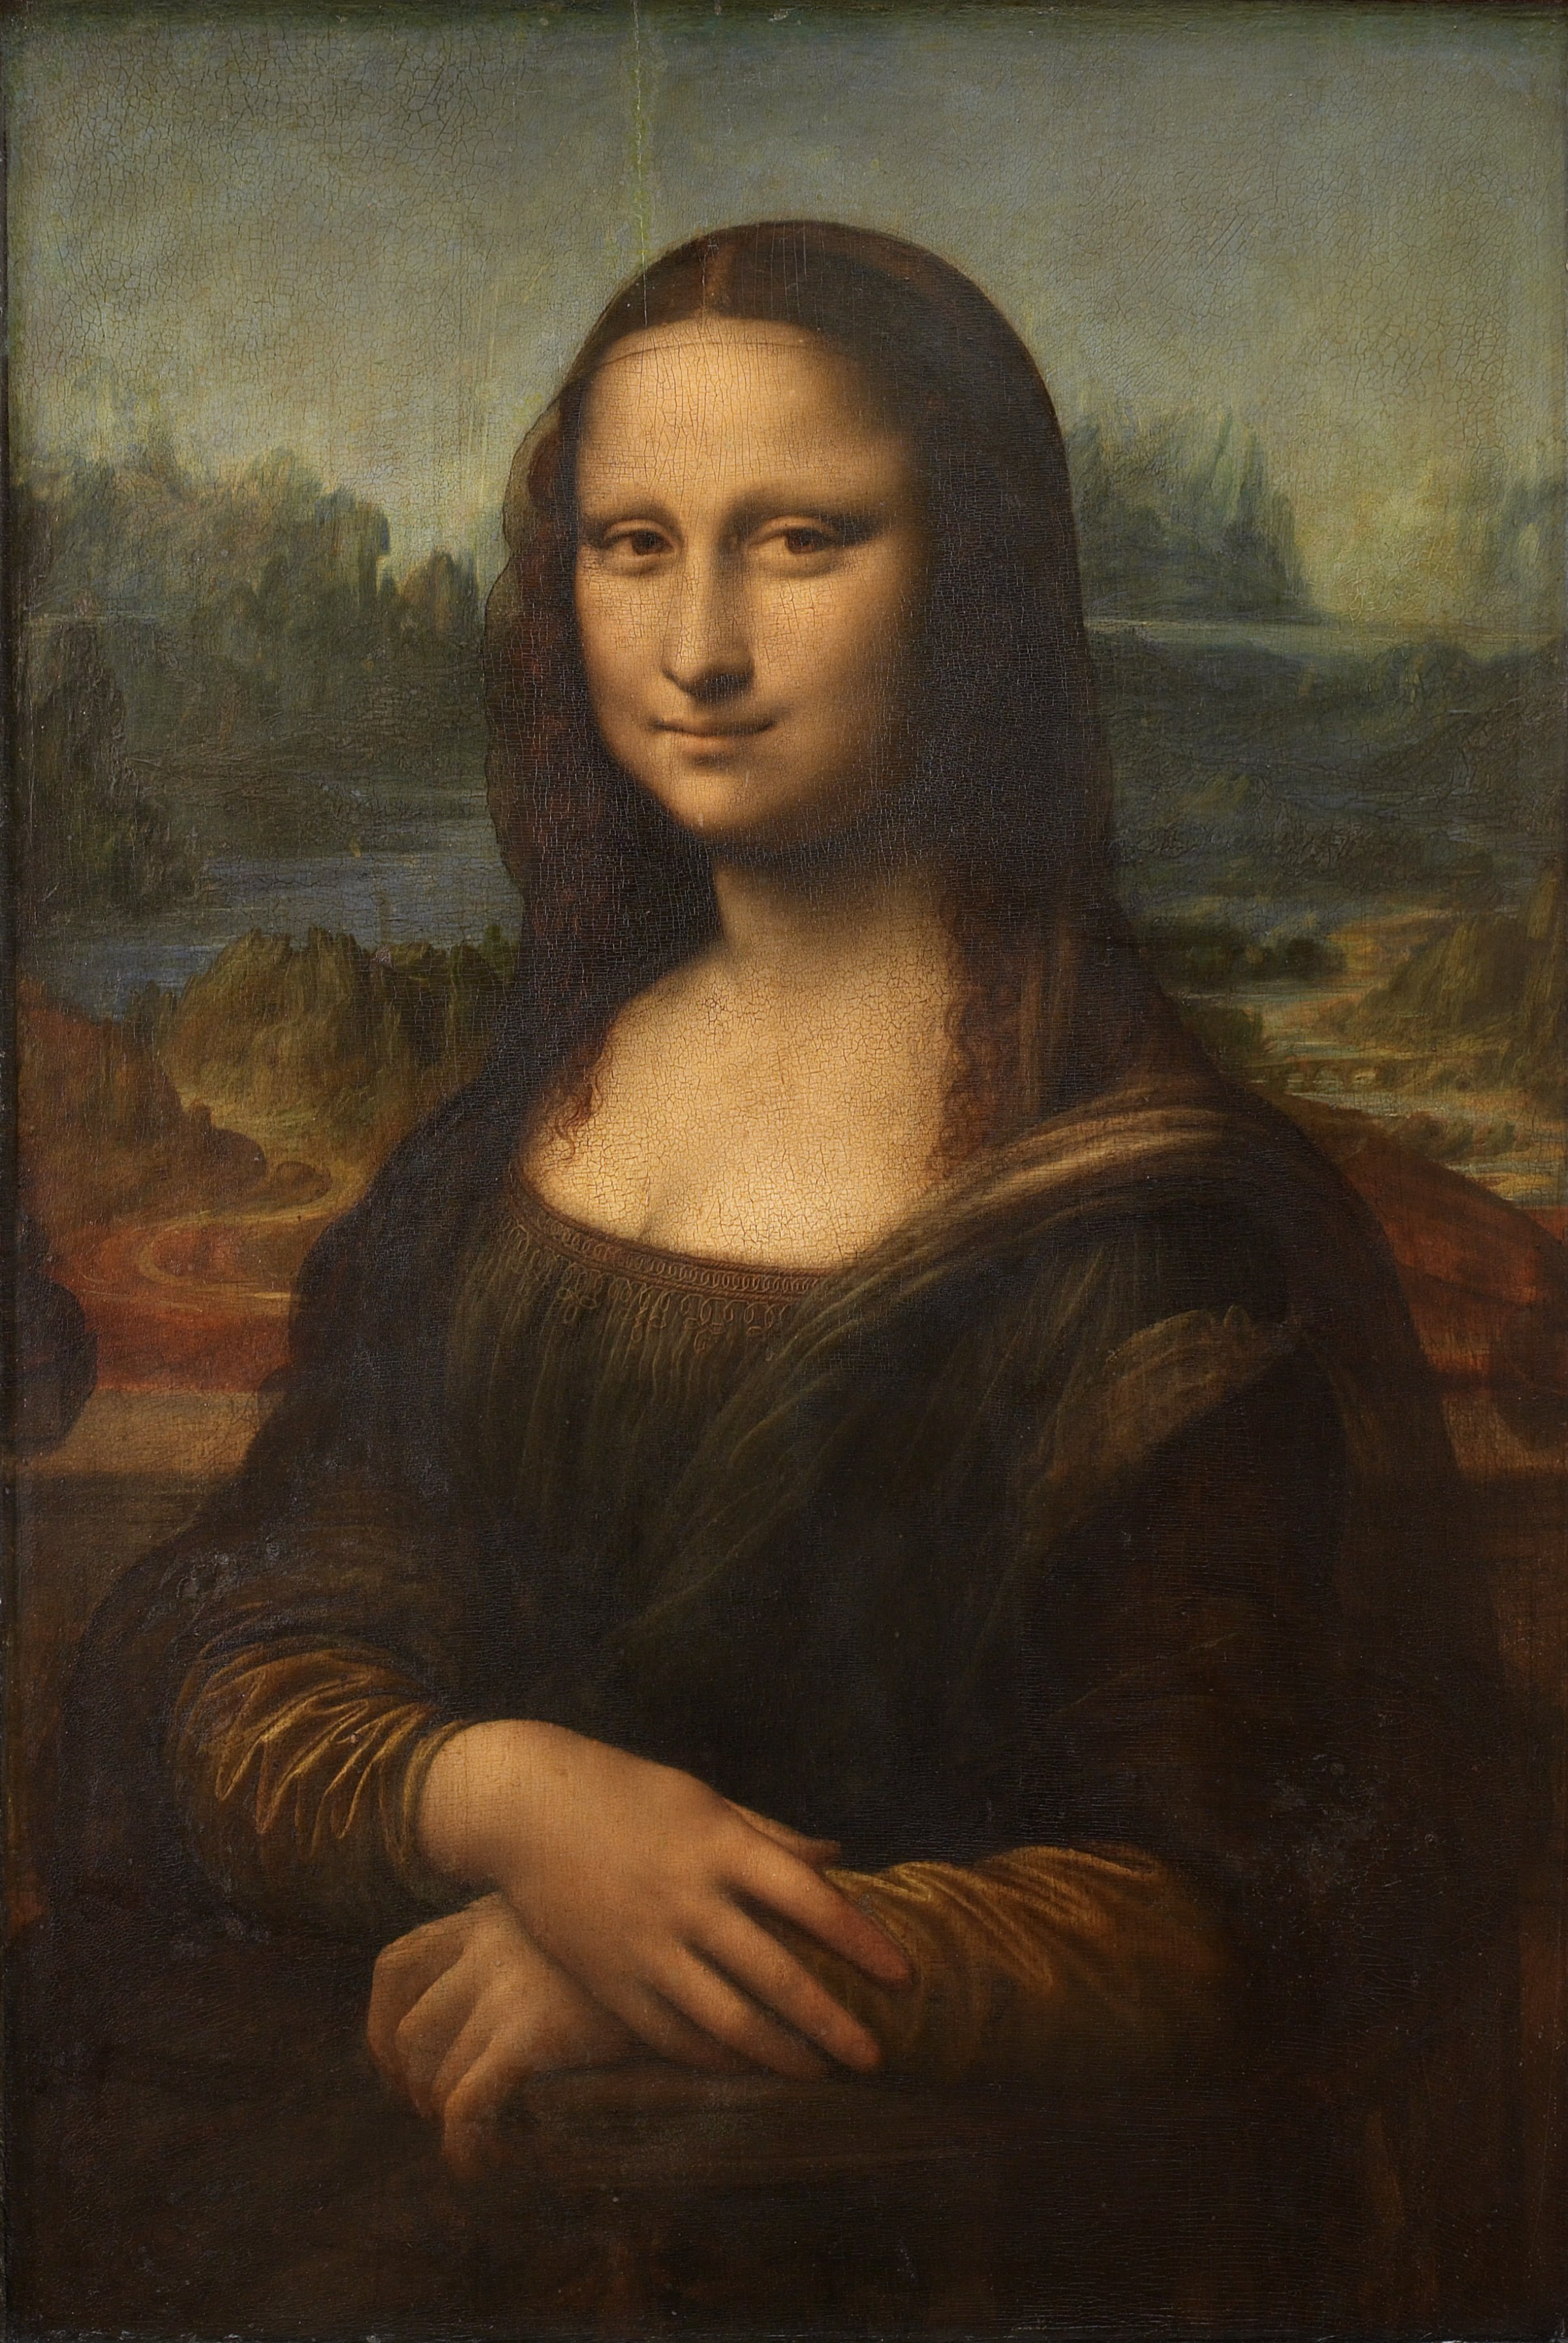
\includegraphics{./images/monalisa.jpeg}
& \\
\begin{minipage}[t]{\linewidth}\raggedright
* unordered list

* Item 2

\begin{itemize}
\item
  sub-item 1
\item
  sub-sub item
\end{itemize}
\end{minipage} & \begin{minipage}[t]{\linewidth}\raggedright
\begin{itemize}
\tightlist
\item
  unordered list
\item
  item 1

  \begin{itemize}
  \tightlist
  \item
    sub-item 1

    \begin{itemize}
    \tightlist
    \item
      sub-sub-item 1
    \end{itemize}
  \end{itemize}
\end{itemize}
\end{minipage} & \\
\begin{minipage}[t]{\linewidth}\raggedright
\begin{enumerate}
\def\labelenumi{\arabic{enumi}.}
\tightlist
\item
  ordered list
\item
  item 2

  \begin{enumerate}
  \def\labelenumii{\roman{enumii})}
  \tightlist
  \item
    sub-item 1 A. sub-sub-item 1
  \end{enumerate}
\end{enumerate}
\end{minipage} & \begin{minipage}[t]{\linewidth}\raggedright
\begin{enumerate}
\def\labelenumi{\arabic{enumi}.}
\tightlist
\item
  ordered list
\item
  item 2

  \begin{enumerate}
  \def\labelenumii{\roman{enumii})}
  \tightlist
  \item
    sub-item 1 A. sub-sub-item 1
  \end{enumerate}
\end{enumerate}
\end{minipage} & \\
inline math: \$E = mc\^{}\{2\}\$ & inline math: \(E=mc^{2}\) & \\
display math:

\$\$E = mc\^{}\{2\}\$\$ & \begin{minipage}[t]{\linewidth}\raggedright
display math:\\
\[E = mc^{2}\]\strut
\end{minipage} & \\
\bottomrule()
\end{longtable}

If you want to add a line break add a line break add an empty line
between your paragraphs, otherwise it will continue as the same text.

Use `\ldots` to add inline code: \texttt{print(hi,\ friend)}

Use ``` to delimit blocks of source code:

\begin{Shaded}
\begin{Highlighting}[]
\NormalTok{\textasciigrave{}\textasciigrave{}\textasciigrave{}}
\NormalTok{print(hi, friend)}
\NormalTok{\textasciigrave{}\textasciigrave{}\textasciigrave{}}
\end{Highlighting}
\end{Shaded}

Making tables in Markdown is not complicated. The most frequently used
table is pipe table it lets you se alignment and captions with
\texttt{:}. Tables can get complicated pretty quickly, if you ever get
stuck refer to
\href{https://quarto.org/docs/authoring/tables.html}{quarto's table
documentation}.

\begin{verbatim}
| Default    | Left    | Middle | Right   | 
|------------|:--------|:------:|--------:|
| Hola       | Gable   | 3.141  | Nile    | 
| Bonjour    | Temple  | 2.718  | Amazon  | 
| Konnichiwa | Chaplin | 4.123  | Yangtze | 

: Table Demonstration
\end{verbatim}

\begin{longtable}[]{@{}llcr@{}}
\caption{Table Demonstration}\tabularnewline
\toprule()
Default & Left & Middle & Right \\
\midrule()
\endfirsthead
\toprule()
Default & Left & Middle & Right \\
\midrule()
\endhead
Hola & Gable & 3.141 & Nile \\
Bonjour & Temple & 2.718 & Amazon \\
Konnichiwa & Chaplin & 4.123 & Yangtze \\
\bottomrule()
\end{longtable}

If you ever feel lost or struggle with formatting, consider using the
visual editor. It provides a familiar interface and is particularly
useful for creating and previewing tables. To adjust options, for
example the number of list options, simply click on the circle icon with
an ellipsis next to it, and a selection menu will appear. In addition to
this, the visual editor offers extensive customization options for other
elements, such as images and tables.

\begin{verbatim}
::: {.callout-note}
You can copy paste (Ctrl + C; Ctrl + V) a picture in Visual Mode!
:::
\end{verbatim}

You can learn more at \href{https://quarto.org/}{Quarto's website}.

\hypertarget{layout-and-references}{%
\chapter{Layout and References}\label{layout-and-references}}

Knitr is a package that takes care of the middle step between evaluating
code and producing pdf/html. The package run your code and places its
output into a final markdown file, which is later converted by pandoc.

Knitr lets you sen cell options that influence code blocks' execution
and output. They are put at the top of a block within comments. For
example:

\begin{Shaded}
\begin{Highlighting}[]
\FunctionTok{plot}\NormalTok{(sunspot.year)}
\FunctionTok{plot}\NormalTok{(uspop)}
\end{Highlighting}
\end{Shaded}

\begin{figure}

\begin{minipage}[t]{0.50\linewidth}

{\centering 

\raisebox{-\height}{

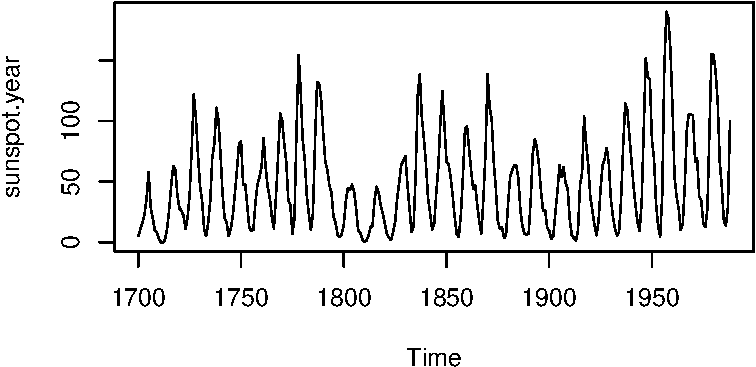
\includegraphics{./layout_refs_files/figure-pdf/fig-plots-1.pdf}

}

}

\subcaption{\label{fig-plots-1}Sunspot}
\end{minipage}%
%
\begin{minipage}[t]{0.50\linewidth}

{\centering 

\raisebox{-\height}{

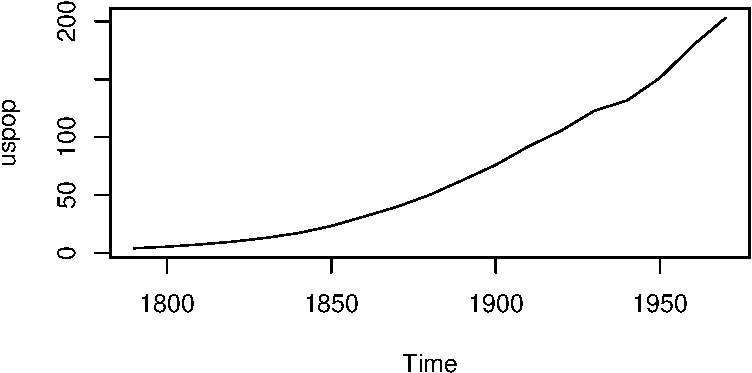
\includegraphics{./layout_refs_files/figure-pdf/fig-plots-2.pdf}

}

}

\subcaption{\label{fig-plots-2}US Population}
\end{minipage}%

\caption{\label{fig-plots}Plots}

\end{figure}

There is large number of options, but I will show the most commonly used
ones. To begin in Figure~\ref{fig-plots}, \texttt{label} is a unique id
for a code cell, which can be referred to in text with
\texttt{@fig-plots}. Similarly, you can refer to tables, chapter, and
files. \texttt{fig-cap} defines a caption for the entire plot.
\texttt{fig-subcap} gives the two plots their individual sub-captions.
\texttt{layout-ncol} let's us display our plots, pictures, etc. in
separate columns. And \texttt{plot()} makes the plots. If you would like
your code to fold use \texttt{code-fold\ =\ true,} above option
\texttt{show} was used to have it opened by default.
\texttt{code-summary} defines text for collapsed code blocks.

Another common options to use within code blocks are:

\begin{longtable}[]{@{}
  >{\raggedright\arraybackslash}p{(\columnwidth - 4\tabcolsep) * \real{0.2639}}
  >{\raggedright\arraybackslash}p{(\columnwidth - 4\tabcolsep) * \real{0.2639}}
  >{\raggedright\arraybackslash}p{(\columnwidth - 4\tabcolsep) * \real{0.4722}}@{}}
\caption{from R Markdown Cheat Sheet}\tabularnewline
\toprule()
\begin{minipage}[b]{\linewidth}\raggedright
Option
\end{minipage} & \begin{minipage}[b]{\linewidth}\raggedright
Value
\end{minipage} & \begin{minipage}[b]{\linewidth}\raggedright
Explanation
\end{minipage} \\
\midrule()
\endfirsthead
\toprule()
\begin{minipage}[b]{\linewidth}\raggedright
Option
\end{minipage} & \begin{minipage}[b]{\linewidth}\raggedright
Value
\end{minipage} & \begin{minipage}[b]{\linewidth}\raggedright
Explanation
\end{minipage} \\
\midrule()
\endhead
eval & true & Whether to evaluate the code and include its results \\
echo & true & Whether to display code along with its results \\
warning & true & Whether to display warnings \\
error & false & Whether to display errors \\
message & true & Whether to display messages \\
include & true & Prevents any output (code, results) from being
included \\
tidy & false & Whether to reformat code in a tidy way when displaying
it \\
results & ``markup'' & Type of output format: ``markup'', ``asis'',
``hold'', or ``hide'' \\
cache & false & Whether to cache results for future renders \\
\bottomrule()
\end{longtable}

\texttt{tidy:\ true} is super useful once you want to include code
inside your document as it will format it nicely.

\hypertarget{div-blocks}{%
\section{Div Blocks}\label{div-blocks}}

If you are familiar with HTML you will recognize
\textless div\textgreater{} blocks. You can add div blocks with wrapping
text in \texttt{:::} or more semicolons. It is useful when you want put
pictures in a grid. Here is a simple example:

\begin{Shaded}
\begin{Highlighting}[]
\NormalTok{::: \{layout{-}ncol="2"\}}
\AlertTok{![Surus](surus.png)}

\AlertTok{![Hanno](hanno.png)}
\NormalTok{:::}
\end{Highlighting}
\end{Shaded}

It must be separated from the preceding and following blocks by blank
lines. Divs can be nested inside other Divs. For example, here we put a
note and some text onto the margin.

\begin{verbatim}
::::: {.column-margin}

::: {.callout-note}
Note!
:::

More text
:::::
\end{verbatim}

\marginnote{\begin{footnotesize}

\begin{tcolorbox}[enhanced jigsaw, toptitle=1mm, opacityback=0, colbacktitle=quarto-callout-note-color!10!white, colback=white, left=2mm, coltitle=black, leftrule=.75mm, breakable, colframe=quarto-callout-note-color-frame, opacitybacktitle=0.6, bottomtitle=1mm, rightrule=.15mm, title=\textcolor{quarto-callout-note-color}{\faInfo}\hspace{0.5em}{Note}, arc=.35mm, titlerule=0mm, bottomrule=.15mm, toprule=.15mm]

Here is a warning.

\end{tcolorbox}

More content.

\end{footnotesize}}

The \texttt{} short code enables you to insert a native page break into
a document that will be compatible with all the other formats:

Because R, YAML, HTML, LaTeX have different notations for commenting.
So, the one that will work universally within quarto is HTML's
\texttt{\textless{}!-\/-\ comment\ here\ -\/-\textgreater{}}.

\hypertarget{diagrams}{%
\section{Diagrams}\label{diagrams}}

You can also create beautiful \href{https://www.uml.org/}{UML} (Unified
Modeling Language) diagrams within quarto with
\href{https://mermaid.js.org/}{Mermaid} and
\href{https://graphviz.org/}{Graphviz}. The flow chart below was maid
with Mermaid!

\begin{verbatim}
flowchart LR
  A[Hard edge] --> B(Round edge)
  B --> C{Decision}
  C --> D[Result one]
  C --> E[Result two]
\end{verbatim}

This might be your first time hearing that there is a language behind
diagrams. UML is a standard graphical notation to describe software
designs. It is a powerful tools for planning, visualizing and documents
your projects. There are different types of diagrams to depict
structures, behaviors and interactions with the standard set of symbols
and notation. We will meet some of them in the chapter on
\protect\hyperlink{relational-databases}{Relational Databases}.

\hypertarget{citations}{%
\section{Citations}\label{citations}}

\begin{quote}
``Proper citation adds credibility to your work and acknowledges the
work of others.'' - \emph{Chat GPT}
\end{quote}

Adding citations to your work shouldn't be stressful or confusing. With
Quarto's seamless integration with Zotero, you can easily add citations
in your preferred style and create a reference list, all without hassle.
How cool is that? I think pretty cool.

Quarto utilizes Pandoc to generate citations and bibliographies in your
preferred style. To source your citations, you'll need a .bib or .bibtex
file, and optionally a .csl file for the citation style. Simply, add
\texttt{bibliography:\ references.bib} to you YAML header in
\texttt{\_quarto.yml}.

\begin{Shaded}
\begin{Highlighting}[]
\FunctionTok{bibliography}\KeywordTok{:}\AttributeTok{ references.bib}
\end{Highlighting}
\end{Shaded}

You can easily cite your article using \texttt{@yourcitation9999}.
Visual mode also provides suggestions, and entering the article's DOI
will help locate and insert it even if it is not in your bibliography.
For more information on citation methods, see
\href{https://quarto.org/docs/authoring/footnotes-and-citations.html}{Quarto
Citation} and \href{https://pandoc.org/MANUAL.html\#citations}{Pandoc
Citations}.

\begin{longtable}[]{@{}
  >{\raggedright\arraybackslash}p{(\columnwidth - 2\tabcolsep) * \real{0.3889}}
  >{\raggedright\arraybackslash}p{(\columnwidth - 2\tabcolsep) * \real{0.6111}}@{}}
\toprule()
\begin{minipage}[b]{\linewidth}\raggedright
Markdown Format
\end{minipage} & \begin{minipage}[b]{\linewidth}\raggedright
Output (author-date format)
\end{minipage} \\
\midrule()
\endhead
@abadie2017 says cluster you SE. & Abadie et al.
(2017)\marginpar{\begin{footnotesize}\leavevmode\vadjust pre{\protect\hypertarget{ref-abadie2017}{}}%
Abadie, Alberto, Susan Athey, Guido Imbens, and Jeffrey Wooldridge.
2017. {``When Should You Adjust Standard Errors for Clustering?''}
Cambridge, MA. \url{https://doi.org/10.3386/w24003}.\vspace{2mm}\par\end{footnotesize}}
says cluster you SE. \\
Some thing smart {[}@abadie2017; @bai2009{]}. & Some thing smart (Abadie
et al. 2017; Bai
2009)\marginpar{\begin{footnotesize}\leavevmode\vadjust pre{\protect\hypertarget{ref-abadie2017}{}}%
Abadie, Alberto, Susan Athey, Guido Imbens, and Jeffrey Wooldridge.
2017. {``When Should You Adjust Standard Errors for Clustering?''}
Cambridge, MA. \url{https://doi.org/10.3386/w24003}.\vspace{2mm}\par\end{footnotesize}}\marginpar{\begin{footnotesize}\leavevmode\vadjust pre{\protect\hypertarget{ref-bai2009}{}}%
Bai, Jushan. 2009. {``Panel Data Models with Interactive Fixed
Effects.''} \emph{Econometrica} 77 (4): 1229--79.
\url{https://doi.org/10.3982/ecta6135}.\vspace{2mm}\par\end{footnotesize}}. \\
Abadie says cluster {[}-@abadie2017{]}. & Abadie says cluster
(2017)\marginpar{\begin{footnotesize}\leavevmode\vadjust pre{\protect\hypertarget{ref-abadie2017}{}}%
Abadie, Alberto, Susan Athey, Guido Imbens, and Jeffrey Wooldridge.
2017. {``When Should You Adjust Standard Errors for Clustering?''}
Cambridge, MA. \url{https://doi.org/10.3386/w24003}.\vspace{2mm}\par\end{footnotesize}}. \\
\bottomrule()
\end{longtable}

If you've successfully created your bibliography in Zotero, adding
citations to your document will be a breeze. Simply start typing and
Zotero will suggest citations to add to your bibliography file. For a
paper with more than 10 citations, I recommend using Better Bibtex,
which allows you to connect citation keys to the paper as you write,
just make sure Zotero is open.

To generate your citations from a document (say cited in Obsidian)
without having to re-cite everything, you can use the
\texttt{bbt\_update\_bib()} function from the
\href{https://github.com/paleolimbot/rbbt}{rbbt} package. Ensure that
Zotero is running and that you're in the markdown document where you
want to update citations. Run the \texttt{bbt\_update\_bib()} function
to create a bibliography, and specify any additional arguments as
needed.

\begin{Shaded}
\begin{Highlighting}[]
\FunctionTok{bbt\_update\_bib}\NormalTok{(}
\NormalTok{  path\_rmd, }\CommentTok{\# Path to your Markdown document.}
  \AttributeTok{path\_bib =} \FunctionTok{bbt\_guess\_bib\_file}\NormalTok{(path\_rmd), }\CommentTok{\# Path to the references.bib file}
  \AttributeTok{translator =} \FunctionTok{bbt\_guess\_translator}\NormalTok{(path\_bib), }\CommentTok{\# type of bibliography file to generate: CSL{-}JSON, BibLaTeX, BibTeX, and CSL YAML.}
\NormalTok{)}
\end{Highlighting}
\end{Shaded}

\part{Collecting the Data}

\hypertarget{qualtrics-api}{%
\chapter{Qualtrics API}\label{qualtrics-api}}

Instead of downloading your data through Qualtrics every time we will
load data using Qualtrics API. For a complete guide refer to this
\href{https://cran.r-project.org/web/packages/qualtRics/vignettes/qualtRics.html}{vignette},
which this guide is based on.

University of San Francisco provides access to Qualtrics; however you
need to separately request API access. Good news, I have talked to ITS
and you should already have it! If not let me know!

First, we need to install a package \texttt{qualtRics}.

\begin{Shaded}
\begin{Highlighting}[]
\FunctionTok{library}\NormalTok{(}\StringTok{"tidyverse"}\NormalTok{)}
\end{Highlighting}
\end{Shaded}

\begin{verbatim}
-- Attaching packages --------------------------------------- tidyverse 1.3.2 --
v ggplot2 3.4.1     v purrr   1.0.1
v tibble  3.1.8     v dplyr   1.1.0
v tidyr   1.3.0     v stringr 1.5.0
v readr   2.1.3     v forcats 0.5.2
-- Conflicts ------------------------------------------ tidyverse_conflicts() --
x dplyr::filter() masks stats::filter()
x dplyr::lag()    masks stats::lag()
\end{verbatim}

\begin{Shaded}
\begin{Highlighting}[]
\FunctionTok{library}\NormalTok{(}\StringTok{"qualtRics"}\NormalTok{)}
\FunctionTok{library}\NormalTok{(}\StringTok{"scales"}\NormalTok{)}
\end{Highlighting}
\end{Shaded}

\begin{verbatim}

Attaching package: 'scales'

The following object is masked from 'package:purrr':

    discard

The following object is masked from 'package:readr':

    col_factor
\end{verbatim}

\begin{Shaded}
\begin{Highlighting}[]
\NormalTok{knitr}\SpecialCharTok{::}\NormalTok{opts\_chunk}\SpecialCharTok{$}\FunctionTok{set}\NormalTok{(}\AttributeTok{echo =}\NormalTok{ T, }\AttributeTok{warning =}\NormalTok{ F, }\AttributeTok{message =}\NormalTok{ F, }\AttributeTok{error =}\NormalTok{ F)}
\end{Highlighting}
\end{Shaded}

\hypertarget{core-functions}{%
\section{Core Functions}\label{core-functions}}

Currently, the package contains three core functions:

\begin{itemize}
\tightlist
\item
  \texttt{all\_surveys()} shows surveys you can access.
\item
  \texttt{fetch\_survey()} downloads the survey.
\item
  \texttt{read\_survey()} reads CSV files you downloaded manually from
  Qualtrics.
\end{itemize}

It also contains a number of helper functions, including:

\begin{itemize}
\tightlist
\item
  \texttt{qualtrics\_api\_credentials()} stores your API key and base
  url in environment variables.
\item
  \texttt{survey\_questions()} retrieves a data frame containing
  questions and question IDs for a survey;
\item
  \texttt{extract\_colmap()} retrieves a similar data frame with more
  detailed mapping from columns to labels.
\item
  \texttt{metadata()} retrieves metadata about your survey, such as
  questions, survey flow, number of responses etc.
\end{itemize}

Note that you can only export surveys that you own, or to which you have
been given administration rights.

\hypertarget{connecting-to-the-api}{%
\section{Connecting to the API}\label{connecting-to-the-api}}

If you have received API access, now you can connect to the API. To get
\texttt{api\_key} and \texttt{base\_url} go to Qualtrics Home Page
\textgreater{} Account Settings \textgreater{} Qualtrics IDs or click
\href{https://usfca.qualtrics.com/Q/QualtricsIdsSection/IdsSection}{this
link}. Under ``API'' click ``Generate Topic'' and you will be issued a
Token. Copy this string a put in ``YOUR\_API\_KEY''. Then look at
``User'' module, copy ``Datacenter ID'' and ``.qualtrics.com'' after it.
Your Base Url should look something like this: ``lad2.qualtrics.com''.

\begin{Shaded}
\begin{Highlighting}[]
\FunctionTok{qualtrics\_api\_credentials}\NormalTok{(}\AttributeTok{api\_key =} \StringTok{"YOUR\_API\_KEY"}\NormalTok{, }
                          \AttributeTok{base\_url =} \StringTok{"YOUR\_BASE\_URL"}\NormalTok{,}
                          \AttributeTok{install =} \ConstantTok{TRUE}\NormalTok{,}
                        \CommentTok{\# overwrite = TRUE \# If you need to update your credentials}
\NormalTok{                          )}
\end{Highlighting}
\end{Shaded}

\begin{Shaded}
\begin{Highlighting}[]
\FunctionTok{qualtrics\_api\_credentials}\NormalTok{(}\AttributeTok{api\_key =} \StringTok{"CEOj8Iwh6BUTNZ9J7PXDJLZpStQaXkmlwLPYzCgu"}\NormalTok{, }
                          \AttributeTok{base\_url =} \StringTok{"lad2.qualtrics.com"}\NormalTok{,}
                          \AttributeTok{install =} \ConstantTok{TRUE}\NormalTok{)}
\end{Highlighting}
\end{Shaded}

After \texttt{qualtrics\_api\_credintials} stored your credentials, you
can use \texttt{all\_surveys()} to fetch information on your surveys.

\begin{Shaded}
\begin{Highlighting}[]
\NormalTok{(surveys }\OtherTok{\textless{}{-}} \FunctionTok{all\_surveys}\NormalTok{()) }
\end{Highlighting}
\end{Shaded}

\begin{verbatim}
# A tibble: 8 x 6
  id                 name                        ownerId lastM~1 creat~2 isAct~3
  <chr>              <chr>                       <chr>   <chr>   <chr>   <lgl>  
1 SV_0rearXjH2Ri6umq Student Satisfaction        UR_2tz~ 2023-0~ 2023-0~ FALSE  
2 SV_2gWVWLn2vCCDJGu Luvuyo                      UR_2tz~ 2022-0~ 2022-0~ FALSE  
3 SV_3h0HPHQbJStqb8a Pilot (USA) - Giver Motive~ UR_2tz~ 2022-0~ 2022-0~ FALSE  
4 SV_3Q011O6gNqwn1Nc Pen Experiment              UR_2tz~ 2022-1~ 2022-1~ FALSE  
5 SV_4YDoTFLN61nKecS Pen_Showcase                UR_2tz~ 2023-0~ 2023-0~ TRUE   
6 SV_4Yhvzriag8syz7U Prosociality Experiment     UR_2tz~ 2023-0~ 2022-0~ FALSE  
7 SV_bJIs8lwz4CfAAgS test                        UR_2tz~ 2023-0~ 2023-0~ TRUE   
8 SV_dnBQ3YB4rLC03J4 test2                       UR_2tz~ 2023-0~ 2023-0~ FALSE  
# ... with abbreviated variable names 1: lastModified, 2: creationDate,
#   3: isActive
\end{verbatim}

Once you select the questionnaire you want you can refer to it using
\texttt{id}. If you want redownload the data set
\texttt{force\_request\ =\ TRUE}, otherwise it will load prior saved
download.

\begin{Shaded}
\begin{Highlighting}[]
\NormalTok{survey\_data }\OtherTok{\textless{}{-}} \FunctionTok{fetch\_survey}\NormalTok{(}\AttributeTok{surveyID =} \StringTok{"SV\_bJIs8lwz4CfAAgS"}\NormalTok{, }
             \AttributeTok{verbose =} \ConstantTok{TRUE}\NormalTok{,}
             \AttributeTok{force\_request =} \ConstantTok{TRUE}\NormalTok{)}
\end{Highlighting}
\end{Shaded}

\begin{verbatim}

  |                                                                            
  |                                                                      |   0%
  |                                                                            
  |======================================================================| 100%
\end{verbatim}

\begin{Shaded}
\begin{Highlighting}[]
\NormalTok{survey\_data }\SpecialCharTok{\%\textgreater{}\%} \FunctionTok{glimpse}\NormalTok{()}
\end{Highlighting}
\end{Shaded}

\begin{verbatim}
Rows: 22
Columns: 89
$ StartDate                 <dttm> 2023-02-07 16:00:52, 2023-02-07 16:01:17, 2~
$ EndDate                   <dttm> 2023-02-07 16:04:08, 2023-02-07 16:04:08, 2~
$ Status                    <chr> "IP Address", "IP Address", "IP Address", "I~
$ IPAddress                 <chr> "138.202.129.171", "138.202.129.164", "138.2~
$ Progress                  <dbl> 100, 100, 100, 100, 100, 100, 100, 100, 100,~
$ `Duration (in seconds)`   <dbl> 196, 171, 104, 187, 189, 198, 210, 209, 180,~
$ Finished                  <lgl> TRUE, TRUE, TRUE, TRUE, TRUE, TRUE, TRUE, TR~
$ RecordedDate              <dttm> 2023-02-07 16:04:09, 2023-02-07 16:04:09, 2~
$ ResponseId                <chr> "R_3r385toH6wjBmyr", "R_2usVBjQ7yXrmY72", "R~
$ RecipientLastName         <lgl> NA, NA, NA, NA, NA, NA, NA, NA, NA, NA, NA, ~
$ RecipientFirstName        <lgl> NA, NA, NA, NA, NA, NA, NA, NA, NA, NA, NA, ~
$ RecipientEmail            <lgl> NA, NA, NA, NA, NA, NA, NA, NA, NA, NA, NA, ~
$ ExternalReference         <lgl> NA, NA, NA, NA, NA, NA, NA, NA, NA, NA, NA, ~
$ LocationLatitude          <dbl> 37.78, 37.78, 37.78, 37.78, 37.78, 37.78, 37~
$ LocationLongitude         <dbl> -122.465, -122.465, -122.465, -122.465, -122~
$ DistributionChannel       <chr> "anonymous", "anonymous", "anonymous", "anon~
$ UserLanguage              <chr> "EN", "EN", "EN", "EN", "EN", "EN", "EN", "E~
$ Consent                   <ord> Yes, Yes, Yes, Yes, Yes, Yes, Yes, Yes, Yes,~
$ Gender                    <ord> Female, Female, Male, Male, Male, Male, Male~
$ Name                      <chr> "Tasha", "Khushboo Patel", "Nikita", "Lawren~
$ Competitive               <ord> Competitive, Competitive, Competitive, Compe~
$ Pizzas_1                  <chr> "Margherita", NA, NA, "Margherita", "Margher~
$ Pizzas_2                  <chr> "Pepperoni", NA, NA, "Pepperoni", "Pepperoni~
$ Pizzas_3                  <chr> NA, "BBQ Chicken", NA, NA, "BBQ Chicken", "B~
$ Pizzas_4                  <chr> "Hawaiian", NA, NA, NA, "Hawaiian", NA, "Haw~
$ Pizzas_5                  <chr> "Veggie", "Veggie", "Veggie", "Veggie", "Veg~
$ Pizzas_6                  <chr> NA, NA, NA, NA, NA, "I also love that one:",~
$ Pizzas_7                  <chr> NA, NA, NA, NA, NA, NA, NA, NA, NA, NA, NA, ~
$ Pizzas_6_TEXT             <chr> NA, NA, NA, NA, NA, "Garlic White Chinese be~
$ Pizzas_DO_1               <dbl> 5, 1, 2, 4, 5, 3, 1, 1, 5, 5, 3, 1, 5, 1, 4,~
$ Pizzas_DO_2               <dbl> 3, 3, 5, 1, 3, 2, 3, 3, 1, 4, 2, 5, 3, 3, 5,~
$ Pizzas_DO_3               <dbl> 2, 2, 3, 5, 4, 1, 4, 5, 2, 2, 1, 3, 1, 2, 2,~
$ Pizzas_DO_4               <dbl> 1, 4, 1, 3, 2, 5, 2, 2, 3, 1, 5, 4, 2, 5, 1,~
$ Pizzas_DO_5               <dbl> 4, 5, 4, 2, 1, 4, 5, 4, 4, 3, 4, 2, 4, 4, 3,~
$ Pizzas_DO_6               <dbl> 6, 6, 6, 6, 6, 6, 6, 6, 6, 6, 6, 6, 6, 6, 6,~
$ Pizzas_DO_7               <dbl> 7, 7, 7, 7, 7, 7, 7, 7, 7, 7, 7, 7, 7, 7, 7,~
$ `1_Taste`                 <dbl> 5, NA, NA, 5, 3, NA, 3, 4, 4, 5, 4, NA, NA, ~
$ `1_Healthiness`           <dbl> 5, NA, NA, 4, 4, NA, 2, 3, 3, 5, 2, NA, NA, ~
$ `1_Ease_Of_Preparation`   <dbl> 5, NA, NA, 4, 4, NA, 4, 3, 4, 3, 3, NA, NA, ~
$ `2_Taste`                 <lgl> NA, NA, NA, NA, NA, NA, NA, NA, NA, NA, NA, ~
$ `2_Healthiness`           <lgl> NA, NA, NA, NA, NA, NA, NA, NA, NA, NA, NA, ~
$ `2_Ease_Of_Preparation`   <lgl> NA, NA, NA, NA, NA, NA, NA, NA, NA, NA, NA, ~
$ `3_Taste`                 <dbl> NA, NA, NA, NA, NA, 4, 5, NA, 4, NA, NA, NA,~
$ `3_Healthiness`           <dbl> NA, NA, NA, NA, NA, 3, 3, NA, 2, NA, NA, NA,~
$ `3_Ease_Of_Preparation`   <dbl> NA, NA, NA, NA, NA, 3, 4, NA, 3, NA, NA, NA,~
$ `9_Taste`                 <dbl> 5, NA, NA, 5, 5, NA, 5, NA, NA, NA, 5, NA, 4~
$ `9_Healthiness`           <dbl> 3, NA, NA, 3, 2, NA, 2, NA, NA, NA, 2, NA, 4~
$ `9_Ease_Of_Preparation`   <dbl> 5, NA, NA, 5, 4, NA, 4, NA, NA, NA, 4, NA, N~
$ `10_Taste`                <dbl> NA, 5, NA, NA, 5, 5, 3, 4, 4, NA, 4, NA, 4, ~
$ `10_Healthiness`          <dbl> NA, NA, NA, NA, 2, 3, 2, 3, 3, NA, 2, NA, 4,~
$ `10_Ease_Of_Preparation`  <dbl> NA, NA, NA, NA, 3, 3, 2, 3, 2, NA, 3, NA, NA~
$ `11_Taste`                <dbl> 5, NA, NA, NA, 4, NA, 5, 4, NA, NA, 4, 5, NA~
$ `11_Healthiness`          <dbl> 4, NA, NA, NA, 2, NA, 2, 3, NA, NA, 3, 4, NA~
$ `11_Ease_Of_Preparation`  <dbl> 5, NA, NA, NA, 3, NA, 3, 2, NA, NA, 2, 3, NA~
$ `12_Taste`                <dbl> 5, 4, 4, 4, 4, NA, 3, NA, NA, NA, 4, NA, NA,~
$ `12_Healthiness`          <dbl> 5, 2, 5, 5, 4, NA, 3, NA, NA, NA, 4, NA, NA,~
$ `12_Ease_Of_Preparation`  <dbl> 4, 3, 3, 3, 2, NA, 2, NA, NA, NA, 3, NA, NA,~
$ `match timer_First Click` <dbl> 0.000, 0.000, 0.000, 0.000, 20.317, 0.000, 0~
$ `match timer_Last Click`  <dbl> 0.000, 0.000, 0.000, 0.000, 20.317, 0.000, 0~
$ `match timer_Page Submit` <dbl> 8.296, 12.572, 7.955, 22.206, 21.188, 7.224,~
$ `match timer_Click Count` <dbl> 0, 0, 0, 0, 1, 0, 0, 0, 0, 0, 0, 0, 1, 0, 0,~
$ transfer                  <dbl> 50, NA, 35, NA, 49, NA, NA, 35, NA, 10, 50, ~
$ `get timer_First Click`   <dbl> 0, 0, 0, 0, 0, 0, 0, 0, 0, 0, 0, 0, 0, 0, 0,~
$ `get timer_Last Click`    <dbl> 0, 0, 0, 0, 0, 0, 0, 0, 0, 0, 0, 0, 0, 0, 0,~
$ `get timer_Page Submit`   <dbl> 4.999, 15.967, 32.000, 2.787, 3.006, 10.538,~
$ `get timer_Click Count`   <dbl> 0, 0, 0, 0, 0, 0, 0, 0, 0, 0, 0, 0, 0, 0, 0,~
$ decision...67             <chr> NA, "I accept A's offer.\n(You get ${e://Fie~
$ Q23                       <ord> Yes, Absolutely, Absolutely, Yes, Yes, Yes, ~
$ researcherID              <chr> "hTtZNw8TA0", "hTtZNw8TA0", "hTtZNw8TA0", "h~
$ studyID                   <chr> "test", "test", "test", "test", "test", "tes~
$ groupID                   <dbl> 6, 6, 5, 5, 7, 7, 8, 8, 9, 9, 10, 10, 11, 11~
$ participantID             <chr> "R_3r385toH6wjBmyr", "R_2usVBjQ7yXrmY72", "R~
$ groupSize                 <dbl> 2, 2, 2, 2, 2, 2, 2, 2, 2, 2, 2, 2, 2, 2, 2,~
$ numStages                 <dbl> 2, 2, 2, 2, 2, 2, 2, 2, 2, 2, 2, 2, 2, 2, 2,~
$ roles                     <chr> "A,B", "A,B", "A,B", "A,B", "A,B", "A,B", "A~
$ participantRole           <chr> "A", "B", "A", "B", "A", "B", "B", "A", "B",~
$ timeOutLog                <chr> "OK -- no issues", "OK -- no issues", "OK --~
$ botMatch                  <chr> "no", "no", "no", "no", "no", "no", "no", "n~
$ total                     <dbl> 100, 100, 100, 100, 100, 100, 100, 100, 100,~
$ offer                     <dbl> 50, 50, 35, 35, 49, 49, 35, 35, 10, 10, 50, ~
$ decision...81             <dbl> 1, 1, 1, 1, 1, 1, 1, 1, 1, 1, 1, 1, 1, 1, 1,~
$ payoff                    <dbl> 50, 50, 65, 35, 51, 49, 35, 65, 10, 90, 50, ~
$ sendStage                 <dbl> 1, 2, 1, 2, 1, 2, 2, 1, 2, 1, 1, 2, 1, 2, 2,~
$ sendData                  <chr> "offer", "decision", "offer", "decision", "o~
$ getStage                  <dbl> 2, 1, 2, 1, 2, 1, 1, 2, 1, 2, 2, 1, 2, 1, 1,~
$ getData                   <chr> "B", "A", "B", "A", "B", "A", "A", "B", "A",~
$ defaultData               <dbl> 2, 20, 2, 5, 2, 71, 61, 1, 83, 2, 2, 81, 1, ~
$ saveData                  <chr> "decision", "offer", "decision", "offer", "d~
$ randomPercent             <dbl> NA, 20, NA, 5, NA, 71, 61, NA, 83, NA, NA, 8~
\end{verbatim}

In case you want to see text of the questions use
\texttt{survey\_questions()}.

\begin{Shaded}
\begin{Highlighting}[]
\NormalTok{survey\_questions }\OtherTok{\textless{}{-}} \FunctionTok{survey\_questions}\NormalTok{(}\AttributeTok{surveyID =} \StringTok{"SV\_bJIs8lwz4CfAAgS"}\NormalTok{)}
\FunctionTok{head}\NormalTok{(survey\_questions, }\AttributeTok{n =} \DecValTok{5}\NormalTok{)}
\end{Highlighting}
\end{Shaded}

\begin{verbatim}
# A tibble: 5 x 4
  qid   qname        question                                            force~1
  <chr> <chr>        <chr>                                               <lgl>  
1 QID25 Introduction "Welcome to the <strong>University of San Francisc~ FALSE  
2 QID26 Consent      "Do you agree to participate in the survey?"        TRUE   
3 QID21 Gender       "What is your gender"                               TRUE   
4 QID23 Name         "What is your Name?"                                FALSE  
5 QID22 Competitive  "Would you consider yourself competitive?"          FALSE  
# ... with abbreviated variable name 1: force_resp
\end{verbatim}

\hypertarget{example}{%
\section{Example}\label{example}}

\begin{Shaded}
\begin{Highlighting}[]
\NormalTok{survey\_data }\OtherTok{\textless{}{-}} \FunctionTok{fetch\_survey}\NormalTok{(}\AttributeTok{surveyID =} \StringTok{"SV\_bJIs8lwz4CfAAgS"}\NormalTok{, }
                            \AttributeTok{verbose =} \ConstantTok{TRUE}\NormalTok{,}\AttributeTok{force\_request =} \ConstantTok{TRUE}\NormalTok{)}
\end{Highlighting}
\end{Shaded}

\begin{verbatim}

  |                                                                            
  |                                                                      |   0%
  |                                                                            
  |======================================================================| 100%
\end{verbatim}

\begin{Shaded}
\begin{Highlighting}[]
\NormalTok{survey\_data }\OtherTok{\textless{}{-}}\NormalTok{ survey\_data }\SpecialCharTok{\%\textgreater{}\%}\NormalTok{ janitor}\SpecialCharTok{::}\FunctionTok{clean\_names}\NormalTok{()}

\NormalTok{graph\_data }\OtherTok{\textless{}{-}}\NormalTok{ survey\_data }\SpecialCharTok{\%\textgreater{}\%}\FunctionTok{select}\NormalTok{(gender, offer,  decision\_81, participant\_id, participant\_role) }\SpecialCharTok{\%\textgreater{}\%} 
  \FunctionTok{mutate}\NormalTok{(}\AttributeTok{participant\_role =} \FunctionTok{recode}\NormalTok{(participant\_role,}\StringTok{"A"} \OtherTok{=} \StringTok{"dictator"}\NormalTok{, }\StringTok{"B"} \OtherTok{=} \StringTok{"recipient"}\NormalTok{ ),}
         \AttributeTok{decision =} \FunctionTok{recode}\NormalTok{(decision\_81, }\StringTok{"1"} \OtherTok{=} \StringTok{"Accepted"}\NormalTok{, }\StringTok{"2"} \OtherTok{=} \StringTok{"Declined"}\NormalTok{)) }\SpecialCharTok{\%\textgreater{}\%} 
  \FunctionTok{mutate}\NormalTok{(}\AttributeTok{interval =} \FunctionTok{cut\_width}\NormalTok{(offer, }\AttributeTok{width =} \DecValTok{10}\NormalTok{, }\AttributeTok{center =} \DecValTok{45}\NormalTok{)) }\SpecialCharTok{\%\textgreater{}\%}
  \FunctionTok{filter}\NormalTok{(participant\_role }\SpecialCharTok{==} \StringTok{"recipient"}\NormalTok{) }\SpecialCharTok{\%\textgreater{}\%} \FunctionTok{count}\NormalTok{(decision, interval) }
\end{Highlighting}
\end{Shaded}

\begin{Shaded}
\begin{Highlighting}[]
\NormalTok{graph\_data }\SpecialCharTok{\%\textgreater{}\%}
  \FunctionTok{ggplot}\NormalTok{(}\FunctionTok{aes}\NormalTok{(}\AttributeTok{x =}\NormalTok{ interval, }\AttributeTok{y =}\NormalTok{ n, }\AttributeTok{fill =} \FunctionTok{as.factor}\NormalTok{(decision))) }\SpecialCharTok{+} 
  \FunctionTok{geom\_col}\NormalTok{(}\AttributeTok{position =} \FunctionTok{position\_stack}\NormalTok{()) }\SpecialCharTok{+} 
  \FunctionTok{theme\_minimal}\NormalTok{(}\AttributeTok{base\_size =} \DecValTok{20}\NormalTok{) }\SpecialCharTok{+} 
  \FunctionTok{scale\_y\_continuous}\NormalTok{(}\AttributeTok{breaks =}\NormalTok{ scales}\SpecialCharTok{::}\FunctionTok{breaks\_extended}\NormalTok{(}\AttributeTok{n =} \FunctionTok{max}\NormalTok{(graph\_data}\SpecialCharTok{$}\NormalTok{n))) }\SpecialCharTok{+} 
  \FunctionTok{theme}\NormalTok{(}\AttributeTok{panel.grid.major.x =} \FunctionTok{element\_blank}\NormalTok{(), }
        \AttributeTok{panel.grid.minor.x =} \FunctionTok{element\_blank}\NormalTok{(),}
        \AttributeTok{legend.position =} \StringTok{"top"}\NormalTok{) }\SpecialCharTok{+}
  \FunctionTok{labs}\NormalTok{(}\AttributeTok{x =} \StringTok{"Offer size"}\NormalTok{, }\AttributeTok{y =} \StringTok{"Count"}\NormalTok{, }\AttributeTok{title =} \StringTok{"Results of the Ultimatum Game"}\NormalTok{, }\AttributeTok{fill =} \StringTok{"Result"}\NormalTok{)}
\end{Highlighting}
\end{Shaded}

\begin{figure}[H]

{\centering 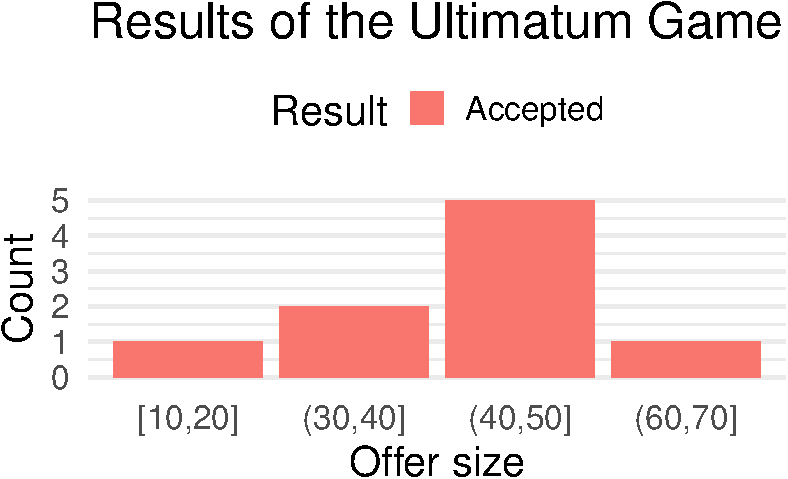
\includegraphics{./qualtrics_api_files/figure-pdf/unnamed-chunk-8-1.pdf}

}

\end{figure}

\begin{Shaded}
\begin{Highlighting}[]
\NormalTok{pizza\_table }\OtherTok{\textless{}{-}}\NormalTok{ survey\_data[}\FunctionTok{c}\NormalTok{(}\DecValTok{22}\SpecialCharTok{:}\DecValTok{29}\NormalTok{,}\DecValTok{72}\NormalTok{)] }\SpecialCharTok{\%\textgreater{}\%} \FunctionTok{select}\NormalTok{(}\SpecialCharTok{{-}}\NormalTok{pizzas\_6) }\SpecialCharTok{\%\textgreater{}\%} \FunctionTok{pivot\_longer}\NormalTok{(}\SpecialCharTok{{-}}\NormalTok{participant\_id) }\SpecialCharTok{\%\textgreater{}\%} \FunctionTok{count}\NormalTok{(value) }\SpecialCharTok{\%\textgreater{}\%} \FunctionTok{drop\_na}\NormalTok{()}
 
\NormalTok{ pizza\_table }\SpecialCharTok{\%\textgreater{}\%} \FunctionTok{ggplot}\NormalTok{(}\FunctionTok{aes}\NormalTok{(}\AttributeTok{x =} \FunctionTok{fct\_reorder}\NormalTok{(value, n), }\AttributeTok{y =}\NormalTok{ n)) }\SpecialCharTok{+} 
   \FunctionTok{geom\_col}\NormalTok{(}\AttributeTok{fill =} \StringTok{"steelblue"}\NormalTok{) }\SpecialCharTok{+} 
   \FunctionTok{theme\_minimal}\NormalTok{(}\AttributeTok{base\_size =} \DecValTok{20}\NormalTok{) }\SpecialCharTok{+} 
   \FunctionTok{scale\_y\_continuous}\NormalTok{(}\AttributeTok{breaks =}\NormalTok{ scales}\SpecialCharTok{::}\FunctionTok{breaks\_extended}\NormalTok{(}\AttributeTok{n =} \FunctionTok{max}\NormalTok{(pizza\_table}\SpecialCharTok{$}\NormalTok{n))) }\SpecialCharTok{+} 
   \FunctionTok{theme}\NormalTok{(}\AttributeTok{panel.grid.major.y =} \FunctionTok{element\_blank}\NormalTok{(), }
         \AttributeTok{panel.grid.minor.y =} \FunctionTok{element\_blank}\NormalTok{(),}
         \AttributeTok{panel.grid.minor.x =} \FunctionTok{element\_blank}\NormalTok{(),}
         \AttributeTok{legend.position =} \StringTok{"top"}\NormalTok{) }\SpecialCharTok{+}
   \FunctionTok{labs}\NormalTok{(}\AttributeTok{x =} \ConstantTok{NULL}\NormalTok{, }\AttributeTok{y =} \StringTok{"Count"}\NormalTok{, }\AttributeTok{title =} \StringTok{"What Pizzas do you like?"}\NormalTok{) }\SpecialCharTok{+} 
   \FunctionTok{coord\_flip}\NormalTok{()}
\end{Highlighting}
\end{Shaded}

\begin{figure}[H]

{\centering 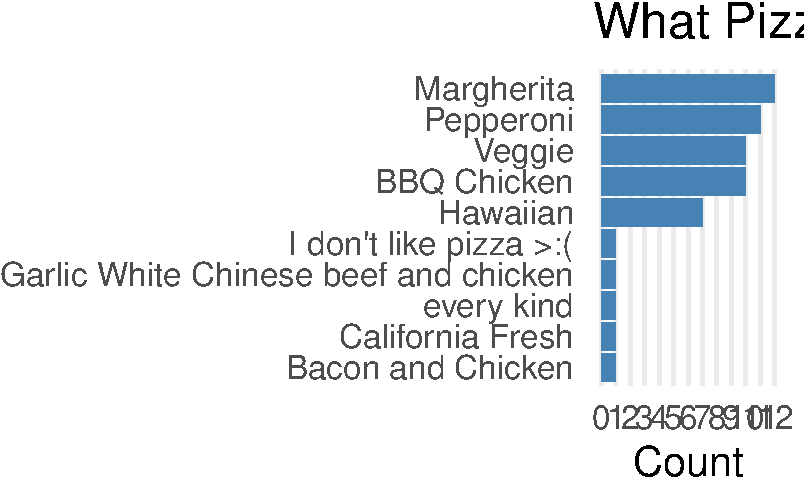
\includegraphics{./qualtrics_api_files/figure-pdf/unnamed-chunk-9-1.pdf}

}

\end{figure}

\part{Working with Data}

\hypertarget{data-manipulation}{%
\chapter{Data Manipulation}\label{data-manipulation}}

Data visualization and manipulation are essential tools for
understanding and communicating complex information in data analysis. R,
a powerful programming language for data analysis, offers a variety of
packages for creating visually appealing plots and manipulating data.
One of the most popular and user-friendly collections of packages for
data visualization and manipulation in R is Tidyverse created by Hadley
Wickham, the Chief Scientist at RStudio. The Tidyverse is a collection
of packages that covers all common tasks, it can be installed using
\texttt{install.packages("tidyverse")} and activated with
\texttt{library("tidyverse")}. In this introduction, we will explore the
basics of using Tidyverse, we will use \texttt{readr} to read data,
\texttt{tidyr} to tidy, \texttt{dplyr} to manipulate, and
\texttt{ggplot2} to visualize. To learn more about the Tidyverse check
out their website \url{https://www.tidyverse.org/}.

Let us start with some basic concepts! We can use R as a basic
calculator

\begin{Shaded}
\begin{Highlighting}[]
\CommentTok{\# This is a comment use "\#" to comment something!}
\DecValTok{2}\SpecialCharTok{+}\DecValTok{2}
\end{Highlighting}
\end{Shaded}

\begin{verbatim}
[1] 4
\end{verbatim}

\begin{Shaded}
\begin{Highlighting}[]
\DecValTok{2}\SpecialCharTok{*}\DecValTok{4} 
\end{Highlighting}
\end{Shaded}

\begin{verbatim}
[1] 8
\end{verbatim}

\begin{Shaded}
\begin{Highlighting}[]
\DecValTok{2}\SpecialCharTok{\^{}}\DecValTok{8}
\end{Highlighting}
\end{Shaded}

\begin{verbatim}
[1] 256
\end{verbatim}

\begin{Shaded}
\begin{Highlighting}[]
\NormalTok{(}\DecValTok{1}\SpecialCharTok{+}\DecValTok{3}\NormalTok{)}\SpecialCharTok{/}\NormalTok{(}\DecValTok{3}\SpecialCharTok{+}\DecValTok{5}\NormalTok{)}
\end{Highlighting}
\end{Shaded}

\begin{verbatim}
[1] 0.5
\end{verbatim}

\begin{Shaded}
\begin{Highlighting}[]
\FunctionTok{log}\NormalTok{(}\DecValTok{10}\NormalTok{) }\CommentTok{\# This takes a natural log of 10! }
\end{Highlighting}
\end{Shaded}

\begin{verbatim}
[1] 2.302585
\end{verbatim}

We can define variables and perform operations on them. R uses
\texttt{=} or \texttt{\textless{}-} to assign values to a variable name.
It is stylistically preferred to use \texttt{\textless{}-} to avoid
confusion and some errors.

\begin{Shaded}
\begin{Highlighting}[]
\NormalTok{x }\OtherTok{\textless{}{-}} \DecValTok{2} \CommentTok{\# same as x = 2}
\NormalTok{x }\SpecialCharTok{*} \DecValTok{4}
\end{Highlighting}
\end{Shaded}

\begin{verbatim}
[1] 8
\end{verbatim}

\texttt{x\ \textless{}-\ 2} stored \texttt{2} in \texttt{x}. Later when
we wrote \texttt{x\ *\ 4} R substituted \texttt{x} for \texttt{2}
evaluating \texttt{2\ *\ 4} to get \texttt{8}. We can update value of
\texttt{x} as much as we want using \texttt{=} or \texttt{\textless{}-}.
Keep in mind R is case sensitive so \texttt{X} and \texttt{x} are
different.

\begin{Shaded}
\begin{Highlighting}[]
\NormalTok{x}
\end{Highlighting}
\end{Shaded}

\begin{verbatim}
[1] 2
\end{verbatim}

\begin{Shaded}
\begin{Highlighting}[]
\NormalTok{x }\OtherTok{\textless{}{-}}\NormalTok{ x }\SpecialCharTok{*} \DecValTok{5}
\end{Highlighting}
\end{Shaded}

\hypertarget{data-types}{%
\subsection{Data Types}\label{data-types}}

R has a number of different data types and classes such as data.frames,
which are similar to excel spreadsheets with columns and rows. We will
first look at vectors. Vectors can hold multiple values of the same
types. Most basic ones are numeric, character and logical.

\begin{Shaded}
\begin{Highlighting}[]
\NormalTok{x}
\end{Highlighting}
\end{Shaded}

\begin{verbatim}
[1] 10
\end{verbatim}

\begin{Shaded}
\begin{Highlighting}[]
\FunctionTok{class}\NormalTok{(x)}
\end{Highlighting}
\end{Shaded}

\begin{verbatim}
[1] "numeric"
\end{verbatim}

\begin{Shaded}
\begin{Highlighting}[]
\NormalTok{(name }\OtherTok{\textless{}{-}} \StringTok{"Parsa Rahimi"}\NormalTok{) }\CommentTok{\# wrapping with (...) will print the variable}
\end{Highlighting}
\end{Shaded}

\begin{verbatim}
[1] "Parsa Rahimi"
\end{verbatim}

\begin{Shaded}
\begin{Highlighting}[]
\FunctionTok{class}\NormalTok{(name)}
\end{Highlighting}
\end{Shaded}

\begin{verbatim}
[1] "character"
\end{verbatim}

\begin{Shaded}
\begin{Highlighting}[]
\NormalTok{(true\_or\_false }\OtherTok{\textless{}{-}} \ConstantTok{TRUE}\NormalTok{)}
\end{Highlighting}
\end{Shaded}

\begin{verbatim}
[1] TRUE
\end{verbatim}

\begin{Shaded}
\begin{Highlighting}[]
\FunctionTok{class}\NormalTok{(true\_or\_false)}
\end{Highlighting}
\end{Shaded}

\begin{verbatim}
[1] "logical"
\end{verbatim}

Note that \texttt{name} is stored as a single character string. What if
we want store name and surname separately in the same object? We can use
concatenate \texttt{c()} to combine objects of similar class into a
vector!

\begin{Shaded}
\begin{Highlighting}[]
\NormalTok{(name\_surname }\OtherTok{\textless{}{-}} \FunctionTok{c}\NormalTok{(}\StringTok{"Parsa"}\NormalTok{,}\StringTok{"Rahimi"}\NormalTok{))}
\end{Highlighting}
\end{Shaded}

\begin{verbatim}
[1] "Parsa"  "Rahimi"
\end{verbatim}

\begin{Shaded}
\begin{Highlighting}[]
\FunctionTok{length}\NormalTok{(name) }
\end{Highlighting}
\end{Shaded}

\begin{verbatim}
[1] 1
\end{verbatim}

\begin{Shaded}
\begin{Highlighting}[]
\FunctionTok{length}\NormalTok{(name\_surname)}
\end{Highlighting}
\end{Shaded}

\begin{verbatim}
[1] 2
\end{verbatim}

Notice how length of the \texttt{name} is 1 and length of the
\texttt{name\_surname} is 2! Let's make a numeric vector and do some
operations on it!

\begin{Shaded}
\begin{Highlighting}[]
\NormalTok{(i }\OtherTok{\textless{}{-}} \FunctionTok{c}\NormalTok{(}\DecValTok{1}\NormalTok{, }\DecValTok{2}\NormalTok{, }\DecValTok{3}\NormalTok{, }\DecValTok{4}\NormalTok{))}
\end{Highlighting}
\end{Shaded}

\begin{verbatim}
[1] 1 2 3 4
\end{verbatim}

\begin{Shaded}
\begin{Highlighting}[]
\NormalTok{i }\SpecialCharTok{+} \DecValTok{10} \CommentTok{\# add 10 to each elements}
\end{Highlighting}
\end{Shaded}

\begin{verbatim}
[1] 11 12 13 14
\end{verbatim}

\begin{Shaded}
\begin{Highlighting}[]
\NormalTok{i }\SpecialCharTok{*} \DecValTok{10} \CommentTok{\# multiply each element by 10}
\end{Highlighting}
\end{Shaded}

\begin{verbatim}
[1] 10 20 30 40
\end{verbatim}

\begin{Shaded}
\begin{Highlighting}[]
\NormalTok{i }\SpecialCharTok{+} \FunctionTok{c}\NormalTok{(}\DecValTok{2}\NormalTok{, }\DecValTok{4}\NormalTok{, }\DecValTok{6}\NormalTok{, }\DecValTok{8}\NormalTok{) }\CommentTok{\# add elements together in matching positions}
\end{Highlighting}
\end{Shaded}

\begin{verbatim}
[1]  3  6  9 12
\end{verbatim}

We haven't modified \texttt{i} with any of those operations. The results
are just printed and not stored. If we want to preserve the results we
have to store them in a variable.

\begin{Shaded}
\begin{Highlighting}[]
\NormalTok{name}
\end{Highlighting}
\end{Shaded}

\begin{verbatim}
[1] "Parsa Rahimi"
\end{verbatim}

\begin{Shaded}
\begin{Highlighting}[]
\NormalTok{name }\OtherTok{\textless{}{-}}\NormalTok{ i }\SpecialCharTok{+} \FunctionTok{c}\NormalTok{(}\DecValTok{5}\NormalTok{,}\DecValTok{4}\NormalTok{,}\DecValTok{2}\NormalTok{,}\DecValTok{1}\NormalTok{)}
\NormalTok{name}
\end{Highlighting}
\end{Shaded}

\begin{verbatim}
[1] 6 6 5 5
\end{verbatim}

Notice that \texttt{name} is no longer ``Parsa Rahimi''. It has been
overwritten by assigning a numeric vector instead of a character string.
But be careful we can perform numeric operations only on numeric objects
otherwise we will receive an error. You can use \texttt{str()} to get
structure of the object such as type, length and other.

\begin{Shaded}
\begin{Highlighting}[]
\NormalTok{name\_surname }\SpecialCharTok{+} \DecValTok{2}
\end{Highlighting}
\end{Shaded}

\begin{verbatim}
Error in name_surname + 2: non-numeric argument to binary operator
\end{verbatim}

\begin{Shaded}
\begin{Highlighting}[]
\FunctionTok{str}\NormalTok{(name\_surname)}
\end{Highlighting}
\end{Shaded}

\begin{verbatim}
 chr [1:2] "Parsa" "Rahimi"
\end{verbatim}

\hypertarget{downloading-data}{%
\section{Downloading Data}\label{downloading-data}}

If you are familiar with Base R (functions that come with the R on
installation) you know about read.csv(). \texttt{readr} provides a
number of function that solve common issues of base R read function.
\texttt{read\_csv} loads data 10 time faster and produces a tibble
instead of a data frame while avoiding inconsistencies of the
\texttt{read.csv}. `Wait what is tibble?' you might ask. Tibbles is
special type of data frame. There are superior to regular data frames as
they load faster, maintain input types, permit columns as lists, allow
non-standard variable names, and never create row names. Okay you have
your data lets load it! First, you need to know the path to your data.
You can go find you file and check its location and then copy paste it.
If you are windows user your path might have ``\textbackslash{}'', which
is an escape character. To fix that replace ``\textbackslash{}'' with
``/''. By copying the path you are getting absolute path
``/Users/User/Documents/your\_project/data/file.csv'' alternatively you
can use local a local path from the folder of the project
``/data/file.csv''. Let's read the data! \texttt{readr::} specifies
which packages to use. Replace the text between ``\ldots{}'' to your
path.

\hypertarget{example-data}{%
\subsection{Example Data}\label{example-data}}

I will be using a sample of experiment's results from Climate and
Cooperation Experiment from Mexico. During the experiments, subjects
were asked to complete three series of ravens matrices, four dictator
games, and a single lottery game. Sessions below 30 Celsius are labeled
as control, and sessions above 30 Celsius as treatment. We will be
primarily using results from Raven's matrices games: 3 sets of 12
matrices. First set, \texttt{pr\_}, is piece-rate round where
participants received points for each correctly solved matrix. Second
set, \texttt{tr\_}, is tournament round where participants competed
againts a random opponent and the winner received double point and the
loser received nothing. Third set, \texttt{ch\_}, is choice round.
Participants were asked to decide whether they want to play piece-rate
or tournament againts a different opponent's score from tournament
round.

You can find data in the \texttt{data} in GitHub repository. We will
need \texttt{tidyverse}.

\begin{Shaded}
\begin{Highlighting}[]
\FunctionTok{library}\NormalTok{(tidyverse)}
\end{Highlighting}
\end{Shaded}

\begin{Shaded}
\begin{Highlighting}[]
\NormalTok{data }\OtherTok{\textless{}{-}}\NormalTok{ readr}\SpecialCharTok{::}\FunctionTok{read\_csv}\NormalTok{(}\StringTok{"https://raw.githubusercontent.com/nikitoshina/ECON{-}623{-}Lab{-}2023/main/data/mexico\_sample\_data.csv?token=GHSAT0AAAAAAB5WTPULI26TZP545VNUFQE6Y6O4XVA"}\NormalTok{) }\CommentTok{\#Download data from git hub}
\end{Highlighting}
\end{Shaded}

We can use \texttt{glimpse()} to get a glimpse at the data. It will give
us a sample and type of the column. Another very common way is to use
\texttt{head()} to get a slice of the top rows or \texttt{tail()} to get
a slice of bottom rows. You can also view the entire data set with
\texttt{View()}

\begin{Shaded}
\begin{Highlighting}[]
\NormalTok{data }\SpecialCharTok{\%\textgreater{}\%} \FunctionTok{glimpse}\NormalTok{()}
\end{Highlighting}
\end{Shaded}

\begin{verbatim}
Rows: 114
Columns: 70
$ id                 <chr> "001018001", "001018002", "001018005", "001018009",~
$ country_city       <chr> "mexico_chapingo", "mexico_chapingo", "mexico_chapi~
$ start_time         <chr> "12H 16M 0S", "12H 16M 0S", "12H 16M 0S", "12H 16M ~
$ end_time           <chr> "13H 14M 0S", "13H 14M 0S", "13H 14M 0S", "13H 14M ~
$ date               <date> 2022-06-20, 2022-06-20, 2022-06-20, 2022-06-20, 20~
$ mean_temp_celsius  <dbl> 28.58772, 28.58772, 28.58772, 28.58772, 28.58772, 2~
$ incentive_local    <dbl> 100, 100, 100, 100, 100, 100, 100, 100, 100, 100, 1~
$ exchange_usd_local <dbl> 20, 20, 20, 20, 20, 20, 20, 20, 20, 20, 20, 20, 20,~
$ incentive_usd      <dbl> 5, 5, 5, 5, 5, 5, 5, 5, 5, 5, 5, 5, 5, 5, 5, 5, 5, ~
$ gender             <chr> "Female", "Male", "Male", "Male", "Male", "Female",~
$ point_value        <dbl> 10, 10, 10, 10, 10, 10, 10, 10, 10, 10, 10, 10, 10,~
$ site_id            <dbl> 1, 1, 1, 1, 1, 1, 1, 1, 1, 1, 1, 1, 1, 1, 1, 1, 1, ~
$ session_n          <dbl> 18, 18, 18, 18, 18, 18, 18, 18, 19, 19, 19, 19, 19,~
$ subject_n          <dbl> 1, 2, 5, 9, 10, 13, 14, 15, 1, 2, 3, 4, 5, 6, 7, 8,~
$ tr_opponet_n       <dbl> 2, 1, 9, 5, 13, 10, 15, 14, 2, 1, 4, 3, 5, 4, 8, 7,~
$ ch_opponent_n      <dbl> 9, NA, NA, 1, 9, NA, NA, NA, NA, 3, 2, NA, NA, 8, N~
$ version            <chr> "A", "A", "A", "A", "A", "A", "A", "A", "A", "A", "~
$ treatment          <dbl> 0, 0, 0, 0, 0, 0, 0, 0, 1, 1, 1, 1, 1, 1, 1, 1, 1, ~
$ dc_cl_ps           <dbl> 1, 1, 1, 1, 1, 1, 1, 1, 1, 1, 1, 1, 1, 1, 1, 1, 1, ~
$ dc_cl_envy         <dbl> 2, 2, 2, 2, 1, 1, 2, 1, 2, 2, 2, 1, 1, 1, 1, 2, 2, ~
$ dc_c_ps            <dbl> 1, 1, 1, 1, 1, 2, 1, 1, 1, 2, 1, 2, 1, 2, 2, 2, 2, ~
$ dc_c_envy          <dbl> 2, 2, 2, 2, 1, 2, 2, 2, 2, 2, 2, 1, 2, 2, 2, 2, 2, ~
$ dc_cl_ps_points    <dbl> 16, 16, 16, 16, 16, 16, 16, 16, 16, 16, 16, 16, 16,~
$ dc_cl_envy_points  <dbl> 20, 20, 20, 20, 16, 16, 16, 20, 20, 20, 16, 20, 16,~
$ dc_c_ps_points     <dbl> 16, 16, 16, 16, 12, 20, 16, 16, 12, 20, 12, 20, 16,~
$ dc_c_envy_points   <dbl> 23, 23, 23, 23, 21, 18, 23, 23, 23, 23, 18, 21, 23,~
$ pr_correct         <dbl> 7, 5, 6, 1, 7, 2, 6, 7, 5, 6, 8, 2, 2, 5, 6, 5, 2, ~
$ pr_wrong           <dbl> 0, 1, 0, 0, 0, 0, 0, 0, 0, 2, 0, 1, 1, 1, 0, 1, 0, ~
$ pr_not_attempted   <dbl> 5, 6, 6, 11, 5, 10, 6, 5, 7, 4, 4, 9, 9, 6, 6, 6, 1~
$ tr_correct         <dbl> 3, 6, 7, 5, 9, 7, 6, 7, 4, 7, 6, 3, 6, 7, 8, 6, 6, ~
$ tr_wrong           <dbl> 1, 1, 1, 4, 0, 0, 2, 1, 2, 2, 2, 0, 3, 1, 1, 4, 1, ~
$ tr_not_attempted   <dbl> 8, 5, 4, 3, 3, 5, 4, 4, 6, 3, 4, 9, 3, 4, 3, 2, 5, ~
$ tr_die             <dbl> 2, 5, 2, 6, 6, 2, 2, 6, 2, 4, 5, 3, 6, 6, 3, 6, 1, ~
$ tr_total           <dbl> 5, 11, 9, 11, 15, 9, 8, 13, 6, 11, 11, 6, 12, 13, 1~
$ tr_guess_correct   <dbl> 5, 7, 8, 6, 11, 5, 8, 5, 5, 6, 8, 5, 5, 8, 8, 7, 3,~
$ tr_guess_die       <dbl> 3, 4, 1, 4, 2, 2, 5, 5, 4, 3, 4, 2, 4, 2, 3, 1, 2, ~
$ tr_guess_total     <dbl> 8, 11, 9, 10, 13, 7, 13, 10, 9, 9, 12, 7, 9, 10, 11~
$ tr_other_correct   <dbl> 6, 3, 5, 7, 7, 9, 7, 6, 7, 4, 3, 6, 6, 3, 6, 8, 8, ~
$ tr_other_die       <dbl> 5, 2, 6, 2, 2, 6, 6, 2, 4, 2, 3, 5, 6, 3, 6, 3, 3, ~
$ tr_other_total     <dbl> 11, 5, 11, 9, 9, 15, 13, 8, 11, 6, 6, 11, 12, 6, 12~
$ tr_result          <dbl> 0, 2, 0, 2, 2, 0, 0, 2, 0, 2, 2, 0, 1, 2, 0, 2, 0, ~
$ tr_points          <dbl> 0, 22, 0, 22, 30, 0, 0, 26, 0, 22, 22, 0, 12, 26, 0~
$ f_happy            <dbl> 5, 9, 8, 4, 8, 8, 3, 7, 6, 10, 8, 9, 4, 5, 9, 8, 6,~
$ f_energetic        <dbl> 7, 8, 7, 3, 10, 9, 3, 5, 7, 10, 9, 8, 5, 6, 9, 6, 8~
$ f_frustrated       <dbl> 8, 3, 3, 0, 4, 8, 8, 2, 7, 0, 3, 0, 5, 0, 1, 2, 0, ~
$ f_last_meal_min    <dbl> 180, 240, 240, 90, 30, 120, 90, 120, 30, 120, 30, 3~
$ ch_correct         <dbl> 9, 4, 7, 7, 10, 5, 7, 6, 4, 4, 8, 6, 5, 6, 6, 6, 5,~
$ ch_wrong           <dbl> 0, 0, 0, 5, 0, 2, 1, 2, 4, 2, 3, 0, 1, 2, 2, 2, 0, ~
$ ch_not_attempted   <dbl> 3, 8, 5, 0, 2, 5, 4, 4, 4, 6, 1, 6, 6, 4, 4, 4, 7, ~
$ ch_die             <dbl> 3, 3, 5, 6, 2, 4, 1, 3, 6, 1, 5, 4, 3, 2, 4, 2, 6, ~
$ ch_total           <dbl> 12, 7, 12, 13, 12, 9, 8, 9, 10, 5, 13, 10, 8, 8, 10~
$ ch_tournament      <dbl> 1, 0, 0, 1, 1, 0, 0, 0, 0, 1, 1, 0, 0, 1, 0, 1, 1, ~
$ ch_other_correct   <dbl> 9, 4, 4, 7, 9, 4, 4, 4, 4, 4, 8, 4, 4, 6, 4, 6, 5, ~
$ ch_other_die       <dbl> 3, 3, 3, 6, 3, 3, 3, 3, 6, 1, 5, 6, 6, 2, 6, 2, 6, ~
$ ch_other_total     <dbl> 12, 7, 7, 13, 12, 7, 7, 7, 10, 5, 13, 10, 10, 8, 10~
$ ch_result          <dbl> 1, NA, NA, 1, 1, NA, NA, NA, NA, 1, 1, NA, NA, 1, N~
$ ch_points          <dbl> 12, 7, 12, 13, 12, 9, 8, 9, 10, 5, 13, 10, 8, 8, 10~
$ ct_selected        <dbl> 2, 2, 3, 6, 6, 2, 1, 1, 1, 6, 2, 1, 1, 1, 6, 6, 6, ~
$ ct_tails           <dbl> 0, 0, 0, 0, 0, 0, 0, 0, 0, 0, 0, 0, 0, 0, 0, 0, 0, ~
$ ct_points          <dbl> 9.5, 9.5, 8.0, 1.0, 1.0, 9.5, 11.0, 11.0, 11.0, 1.0~
$ task_paid          <dbl> 4, 4, 4, 4, 4, 4, 4, 4, 6, 6, 6, 6, 6, 6, 6, 6, 6, ~
$ complete           <dbl> 1, 1, 1, 1, 1, 1, 1, 1, 1, 1, 1, 1, 1, 1, 1, 1, 1, ~
$ total_points       <dbl> 23, 23, 23, 23, 21, 18, 23, 23, 0, 22, 22, 0, 12, 2~
$ total_local_paid   <dbl> 330, 330, 330, 330, 310, 280, 330, 330, 100, 320, 3~
$ total_usd_paid     <dbl> 16.5, 16.5, 16.5, 16.5, 15.5, 14.0, 16.5, 16.5, 5.0~
$ final_version      <dbl> 1, 1, 1, 1, 1, 1, 1, 1, 1, 1, 1, 1, 1, 1, 1, 1, 1, ~
$ comment            <lgl> NA, NA, NA, NA, NA, NA, NA, NA, NA, NA, NA, NA, NA,~
$ f_last_meal_time   <chr> "3 0", "4 0", "4 0", "1 30", "0 30", "2 0", "1 30",~
$ start_time_h       <dbl> 12, 12, 12, 12, 12, 12, 12, 12, 14, 14, 14, 14, 14,~
$ end_time_h         <dbl> 13, 13, 13, 13, 13, 13, 13, 13, 15, 15, 15, 15, 15,~
\end{verbatim}

\hypertarget{basic-data-management}{%
\section{Basic Data Management}\label{basic-data-management}}

dplyr uses a collection of verbs to manipulate data that are piped
(chained) into each other with a piping operator
\texttt{\%\textgreater{}\%} from \texttt{magrittr} package. The way you
use functions in base R is you wrap new function over the previous one,
such as \texttt{k(g(f(x)))} this will become impossible to read very
quickly as you stack up functions and their arguments. To solve this we
will use pipes
\texttt{x\ \%\textgreater{}\%\ f()\ \%\textgreater{}\%\ g()\ \%\textgreater{}\%\ k()}!
Now you can clearly see that we take x and apply f(), then g(), then
k(). Note: base R now also has its own pipe
\texttt{\textbar{}\textgreater{}}, but we will stick to
\texttt{\%\textgreater{}\%} for compatibility across packages.

\hypertarget{select}{%
\subsection{\texorpdfstring{\texttt{select()}}{select()}}\label{select}}

\texttt{select()} selects only the columns that you want, removing all
other columns. You can use column position (with numbers) or name. The
columns will be displayed in the order you list them. We will select
subject\_id, temperature, gender and results of raven's matrices games.

\begin{itemize}
\tightlist
\item
  \texttt{id} is a unique subject identification number, where
  site\_id.session\_n.subject\_n (001.001.001).
\item
  \texttt{mean\_temp\_celsius} is mean temperature through the session
\item
  \texttt{gender} is gender of the subject.
\item
  \texttt{pr\_correct} is number of correct answers in \emph{piece-rate}
  round.
\item
  \texttt{tr\_correct} is number of correct answers in \emph{tournament}
  round.
\item
  \texttt{ch\_correct} is number of correct answers in \emph{choice}
  round.
\item
  \texttt{ch\_tournament} is 1 if participant decided to play tournament
  and 0 if choice.
\end{itemize}

\begin{Shaded}
\begin{Highlighting}[]
\NormalTok{data\_raven }\OtherTok{\textless{}{-}}\NormalTok{ data }\SpecialCharTok{\%\textgreater{}\%} \FunctionTok{select}\NormalTok{(id, mean\_temp\_celsius,gender, pr\_correct, tr\_correct, ch\_tournament, ch\_correct) }
\FunctionTok{head}\NormalTok{(data\_raven)}
\end{Highlighting}
\end{Shaded}

\begin{verbatim}
# A tibble: 6 x 7
  id        mean_temp_celsius gender pr_correct tr_correct ch_tournament ch_co~1
  <chr>                 <dbl> <chr>       <dbl>      <dbl>         <dbl>   <dbl>
1 001018001              28.6 Female          7          3             1       9
2 001018002              28.6 Male            5          6             0       4
3 001018005              28.6 Male            6          7             0       7
4 001018009              28.6 Male            1          5             1       7
5 001018010              28.6 Male            7          9             1      10
6 001018013              28.6 Female          2          7             0       5
# ... with abbreviated variable name 1: ch_correct
\end{verbatim}

You can also exclude columns or select everything else with select using
\texttt{-}

\begin{Shaded}
\begin{Highlighting}[]
\NormalTok{data\_raven }\SpecialCharTok{\%\textgreater{}\%} \FunctionTok{select}\NormalTok{(}\SpecialCharTok{{-}}\NormalTok{gender) }\SpecialCharTok{\%\textgreater{}\%} \FunctionTok{head}\NormalTok{()}
\end{Highlighting}
\end{Shaded}

\begin{verbatim}
# A tibble: 6 x 6
  id        mean_temp_celsius pr_correct tr_correct ch_tournament ch_correct
  <chr>                 <dbl>      <dbl>      <dbl>         <dbl>      <dbl>
1 001018001              28.6          7          3             1          9
2 001018002              28.6          5          6             0          4
3 001018005              28.6          6          7             0          7
4 001018009              28.6          1          5             1          7
5 001018010              28.6          7          9             1         10
6 001018013              28.6          2          7             0          5
\end{verbatim}

\hypertarget{filter}{%
\subsection{\texorpdfstring{\texttt{filter()}}{filter()}}\label{filter}}

\texttt{filter()} keeps only rows that meet the specified criteria.
Let's filter and make 2 data sets one for Males and, one for Females.

\begin{Shaded}
\begin{Highlighting}[]
\NormalTok{data\_male }\OtherTok{\textless{}{-}}\NormalTok{ data\_raven }\SpecialCharTok{\%\textgreater{}\%} \FunctionTok{filter}\NormalTok{(gender }\SpecialCharTok{==} \StringTok{"Male"}\NormalTok{) }\CommentTok{\# we use == for comparison}
\NormalTok{data\_female }\OtherTok{\textless{}{-}}\NormalTok{ data\_raven }\SpecialCharTok{\%\textgreater{}\%} \FunctionTok{filter}\NormalTok{(gender }\SpecialCharTok{==} \StringTok{"Female"}\NormalTok{)}
\FunctionTok{head}\NormalTok{(data\_male)}
\end{Highlighting}
\end{Shaded}

\begin{verbatim}
# A tibble: 6 x 7
  id        mean_temp_celsius gender pr_correct tr_correct ch_tournament ch_co~1
  <chr>                 <dbl> <chr>       <dbl>      <dbl>         <dbl>   <dbl>
1 001018002              28.6 Male            5          6             0       4
2 001018005              28.6 Male            6          7             0       7
3 001018009              28.6 Male            1          5             1       7
4 001018010              28.6 Male            7          9             1      10
5 001019002              30.7 Male            6          7             1       4
6 001019008              30.7 Male            5          6             1       6
# ... with abbreviated variable name 1: ch_correct
\end{verbatim}

\begin{Shaded}
\begin{Highlighting}[]
\FunctionTok{head}\NormalTok{(data\_female)}
\end{Highlighting}
\end{Shaded}

\begin{verbatim}
# A tibble: 6 x 7
  id        mean_temp_celsius gender pr_correct tr_correct ch_tournament ch_co~1
  <chr>                 <dbl> <chr>       <dbl>      <dbl>         <dbl>   <dbl>
1 001018001              28.6 Female          7          3             1       9
2 001018013              28.6 Female          2          7             0       5
3 001018014              28.6 Female          6          6             0       7
4 001018015              28.6 Female          7          7             0       6
5 001019001              30.7 Female          5          4             0       4
6 001019003              30.7 Female          8          6             1       8
# ... with abbreviated variable name 1: ch_correct
\end{verbatim}

We can chain multiple requirements. Here we will look at Males,
temperature over 30 celsius or Females, temperature below 30. Notice
that we use \texttt{\&} as ``and'', \texttt{\textbar{}} as ``or, and
wrap the two conditions into''()'' to avoid confusion. It could read it
as
\texttt{mean\_temp\_celsius\ \textgreater{}\ 30\ \textbar{}\ gender\ ==\ "Female"}.

\begin{Shaded}
\begin{Highlighting}[]
\NormalTok{data\_raven }\SpecialCharTok{\%\textgreater{}\%} 
  \FunctionTok{filter}\NormalTok{( }
\NormalTok{    (gender }\SpecialCharTok{==} \StringTok{"Male"} \SpecialCharTok{\&}\NormalTok{ mean\_temp\_celsius }\SpecialCharTok{\textgreater{}} \DecValTok{30}\NormalTok{) }\SpecialCharTok{|}\NormalTok{ (gender }\SpecialCharTok{==} \StringTok{"Female"} \SpecialCharTok{\&}\NormalTok{ mean\_temp\_celsius }\SpecialCharTok{\textless{}} \DecValTok{30}\NormalTok{)}
\NormalTok{        )}
\end{Highlighting}
\end{Shaded}

\begin{verbatim}
# A tibble: 61 x 7
   id        mean_temp_celsius gender pr_correct tr_correct ch_tournam~1 ch_co~2
   <chr>                 <dbl> <chr>       <dbl>      <dbl>        <dbl>   <dbl>
 1 001018001              28.6 Female          7          3            1       9
 2 001018013              28.6 Female          2          7            0       5
 3 001018014              28.6 Female          6          6            0       7
 4 001018015              28.6 Female          7          7            0       6
 5 001019002              30.7 Male            6          7            1       4
 6 001019008              30.7 Male            5          6            1       6
 7 001019009              30.7 Male            2          6            1       5
 8 001019010              30.7 Male            6          8            0       8
 9 001019011              30.7 Male            7          7            1       7
10 001019012              30.7 Male            4          5            1       6
# ... with 51 more rows, and abbreviated variable names 1: ch_tournament,
#   2: ch_correct
\end{verbatim}

\hypertarget{arrange}{%
\subsection{\texorpdfstring{\texttt{arrange()}}{arrange()}}\label{arrange}}

\texttt{arrange()} allows you to order the table using a variable. Let's
see which subject scored the worst in \texttt{pr\_correct}.

\begin{Shaded}
\begin{Highlighting}[]
\NormalTok{data\_raven }\SpecialCharTok{\%\textgreater{}\%} \FunctionTok{arrange}\NormalTok{(pr\_correct) }\SpecialCharTok{\%\textgreater{}\%} \FunctionTok{head}\NormalTok{()}
\end{Highlighting}
\end{Shaded}

\begin{verbatim}
# A tibble: 6 x 7
  id        mean_temp_celsius gender pr_correct tr_correct ch_tournament ch_co~1
  <chr>                 <dbl> <chr>       <dbl>      <dbl>         <dbl>   <dbl>
1 001018009              28.6 Male            1          5             1       7
2 001018013              28.6 Female          2          7             0       5
3 001019004              30.7 Female          2          3             0       6
4 001019005              30.7 Female          2          6             0       5
5 001019009              30.7 Male            2          6             1       5
6 001021013              30.4 Male            2          3             1       2
# ... with abbreviated variable name 1: ch_correct
\end{verbatim}

We can also sort in descending order using \texttt{desc()} modifier.
Let's look at who scored the most!

\begin{Shaded}
\begin{Highlighting}[]
\NormalTok{data\_raven }\SpecialCharTok{\%\textgreater{}\%} \FunctionTok{arrange}\NormalTok{(}\FunctionTok{desc}\NormalTok{(pr\_correct)) }\SpecialCharTok{\%\textgreater{}\%} \FunctionTok{head}\NormalTok{()}
\end{Highlighting}
\end{Shaded}

\begin{verbatim}
# A tibble: 6 x 7
  id        mean_temp_celsius gender pr_correct tr_correct ch_tournament ch_co~1
  <chr>                 <dbl> <chr>       <dbl>      <dbl>         <dbl>   <dbl>
1 001019003              30.7 Female          8          6             1       8
2 001020002              31.6 Male            8          6             1       5
3 001020013              31.6 Male            8          7             0       7
4 001021006              30.4 Male            8          4             0       7
5 001025009              26.8 Male            8          9             1       9
6 001027015              32.2 Female          8          7             0       8
# ... with abbreviated variable name 1: ch_correct
\end{verbatim}

\hypertarget{mutate}{%
\subsection{\texorpdfstring{\texttt{mutate()}}{mutate()}}\label{mutate}}

\texttt{mutate()} adds new columns and modifies current variables in the
data set. Let's create a dataset with 10 rows and make three new
variable columns as an example

\begin{Shaded}
\begin{Highlighting}[]
\FunctionTok{tibble}\NormalTok{(}\AttributeTok{rows =} \DecValTok{1}\SpecialCharTok{:}\DecValTok{10}\NormalTok{) }\SpecialCharTok{\%\textgreater{}\%} \FunctionTok{mutate}\NormalTok{(}
  \AttributeTok{One =} \DecValTok{1}\NormalTok{,}
  \AttributeTok{Comment =} \StringTok{"Something"}\NormalTok{,}
  \AttributeTok{Approved =} \ConstantTok{TRUE}
\NormalTok{)}
\end{Highlighting}
\end{Shaded}

\begin{verbatim}
# A tibble: 10 x 4
    rows   One Comment   Approved
   <int> <dbl> <chr>     <lgl>   
 1     1     1 Something TRUE    
 2     2     1 Something TRUE    
 3     3     1 Something TRUE    
 4     4     1 Something TRUE    
 5     5     1 Something TRUE    
 6     6     1 Something TRUE    
 7     7     1 Something TRUE    
 8     8     1 Something TRUE    
 9     9     1 Something TRUE    
10    10     1 Something TRUE    
\end{verbatim}

\texttt{mutate()} can use existing variables from the data set to create
new ones! Lets convert Celsius to Fahrenheit, see how many point more
people scored in tournament over piece-rate round, and check how far
from the mean they scored in piece-rate round!

\begin{Shaded}
\begin{Highlighting}[]
\NormalTok{data\_raven }\SpecialCharTok{\%\textgreater{}\%} \FunctionTok{mutate}\NormalTok{(}\AttributeTok{mean\_temp\_fahrenheit =}\NormalTok{ (mean\_temp\_celsius }\SpecialCharTok{*} \DecValTok{9}\SpecialCharTok{/}\DecValTok{5}\NormalTok{) }\SpecialCharTok{+} \DecValTok{32}\NormalTok{,}
                      \AttributeTok{impovement =}\NormalTok{ tr\_correct }\SpecialCharTok{{-}}\NormalTok{ pr\_correct,}
                      \AttributeTok{pr\_deviation =}\NormalTok{ pr\_correct }\SpecialCharTok{{-}} \FunctionTok{mean}\NormalTok{(pr\_correct))}
\end{Highlighting}
\end{Shaded}

\begin{verbatim}
# A tibble: 114 x 10
   id     mean_~1 gender pr_co~2 tr_co~3 ch_to~4 ch_co~5 mean_~6 impov~7 pr_de~8
   <chr>    <dbl> <chr>    <dbl>   <dbl>   <dbl>   <dbl>   <dbl>   <dbl>   <dbl>
 1 00101~    28.6 Female       7       3       1       9    83.5      -4   1.66 
 2 00101~    28.6 Male         5       6       0       4    83.5       1  -0.342
 3 00101~    28.6 Male         6       7       0       7    83.5       1   0.658
 4 00101~    28.6 Male         1       5       1       7    83.5       4  -4.34 
 5 00101~    28.6 Male         7       9       1      10    83.5       2   1.66 
 6 00101~    28.6 Female       2       7       0       5    83.5       5  -3.34 
 7 00101~    28.6 Female       6       6       0       7    83.5       0   0.658
 8 00101~    28.6 Female       7       7       0       6    83.5       0   1.66 
 9 00101~    30.7 Female       5       4       0       4    87.2      -1  -0.342
10 00101~    30.7 Male         6       7       1       4    87.2       1   0.658
# ... with 104 more rows, and abbreviated variable names 1: mean_temp_celsius,
#   2: pr_correct, 3: tr_correct, 4: ch_tournament, 5: ch_correct,
#   6: mean_temp_fahrenheit, 7: impovement, 8: pr_deviation
\end{verbatim}

Notice that we can nest functions within \texttt{mutate()}: first we
took \texttt{mean()} of the entire column and then subtracted it from
\texttt{pr\_correct}.

\hypertarget{recode}{%
\subsection{\texorpdfstring{\texttt{recode()}}{recode()}}\label{recode}}

\texttt{recode()} modifies the values within a variable. Here is a
template:

\begin{quote}
data \%\textgreater\% mutate(Variable = recode(Variable, ``old value'' =
``new value''))
\end{quote}

Let's use \texttt{recode()} to change ``Male'' to ``M'' and ``Female''
to ``F''.

\begin{Shaded}
\begin{Highlighting}[]
\NormalTok{data\_raven }\OtherTok{\textless{}{-}}\NormalTok{ data\_raven }\SpecialCharTok{\%\textgreater{}\%} \FunctionTok{mutate}\NormalTok{(}\AttributeTok{gender =} \FunctionTok{recode}\NormalTok{(gender, }\StringTok{"Male"} \OtherTok{=} \StringTok{"M"}\NormalTok{, }\StringTok{"Female"} \OtherTok{=} \StringTok{"F"}\NormalTok{))}
\end{Highlighting}
\end{Shaded}

\hypertarget{summarize}{%
\section{\texorpdfstring{\texttt{summarize()}}{summarize()}}\label{summarize}}

\texttt{summarize()} collapses all rows and returns a one-row summary.
We will use summary to calculation what percentage of participant were
male, median score in piece-rate round, max score in tournament,
percentage of people choosing tournament in choice and mean score in
choice round.

\begin{Shaded}
\begin{Highlighting}[]
\NormalTok{data\_raven }\SpecialCharTok{\%\textgreater{}\%} 
  \FunctionTok{summarize}\NormalTok{(}\AttributeTok{perc\_male =} \FunctionTok{sum}\NormalTok{(gender }\SpecialCharTok{==} \StringTok{"Male"}\NormalTok{, }\AttributeTok{na.rm =}\NormalTok{ T) }\SpecialCharTok{/} \FunctionTok{n}\NormalTok{(),}
            \AttributeTok{pr\_median =} \FunctionTok{median}\NormalTok{(pr\_correct),}
            \AttributeTok{tr\_max =} \FunctionTok{max}\NormalTok{(tr\_correct),}
            \AttributeTok{ch\_ratio =} \FunctionTok{sum}\NormalTok{(ch\_tournament) }\SpecialCharTok{/} \FunctionTok{n}\NormalTok{(),}
            \AttributeTok{ch\_mean =} \FunctionTok{mean}\NormalTok{(ch\_correct))}
\end{Highlighting}
\end{Shaded}

\begin{verbatim}
# A tibble: 1 x 5
  perc_male pr_median tr_max ch_ratio ch_mean
      <dbl>     <dbl>  <dbl>    <dbl>   <dbl>
1         0         5      9    0.456    6.01
\end{verbatim}

\hypertarget{group_by-and-ungroup}{%
\section{\texorpdfstring{\texttt{group\_by()} and
\texttt{ungroup()}}{group\_by() and ungroup()}}\label{group_by-and-ungroup}}

\hypertarget{group_by}{%
\subsection{\texorpdfstring{\texttt{group\_by()}}{group\_by()}}\label{group_by}}

\texttt{group\_by()} groups data by specific variables for future
operations. We can use \texttt{group\_by()} and \texttt{summarize()} to
calculate different summary statistics for genders!

\begin{Shaded}
\begin{Highlighting}[]
\NormalTok{data\_raven }\SpecialCharTok{\%\textgreater{}\%} 
  \FunctionTok{drop\_na}\NormalTok{(gender) }\SpecialCharTok{\%\textgreater{}\%}  \CommentTok{\# removes NA gender}
  \FunctionTok{group\_by}\NormalTok{(gender) }\SpecialCharTok{\%\textgreater{}\%} 
  \FunctionTok{summarize}\NormalTok{(}\AttributeTok{pr\_mean =} \FunctionTok{mean}\NormalTok{(pr\_correct),}
            \AttributeTok{tr\_mean =} \FunctionTok{mean}\NormalTok{(tr\_correct),}
            \AttributeTok{ch\_mean =} \FunctionTok{mean}\NormalTok{(ch\_correct),}
            \AttributeTok{pr\_sd =} \FunctionTok{sd}\NormalTok{(pr\_correct),}
            \AttributeTok{n =} \FunctionTok{n}\NormalTok{()) }\SpecialCharTok{\%\textgreater{}\%}
  \FunctionTok{ungroup}\NormalTok{()}
\end{Highlighting}
\end{Shaded}

\begin{verbatim}
# A tibble: 2 x 6
  gender pr_mean tr_mean ch_mean pr_sd     n
  <chr>    <dbl>   <dbl>   <dbl> <dbl> <int>
1 F         5.22    6.17    5.93  1.58    58
2 M         5.47    6.4     6.09  1.59    55
\end{verbatim}

Let's group by gender and choice in choice round and look at points in
choice round!

\begin{Shaded}
\begin{Highlighting}[]
\NormalTok{data\_raven }\SpecialCharTok{\%\textgreater{}\%}
  \FunctionTok{drop\_na}\NormalTok{(gender) }\SpecialCharTok{\%\textgreater{}\%}  \CommentTok{\# removes NA gender}
  \FunctionTok{group\_by}\NormalTok{(gender, ch\_tournament) }\SpecialCharTok{\%\textgreater{}\%} 
  \FunctionTok{summarize}\NormalTok{(}\AttributeTok{ch\_mean =} \FunctionTok{mean}\NormalTok{(ch\_correct),}
            \AttributeTok{pr\_sd =} \FunctionTok{sd}\NormalTok{(ch\_correct),}
            \AttributeTok{n =} \FunctionTok{n}\NormalTok{()) }\SpecialCharTok{\%\textgreater{}\%}
  \FunctionTok{ungroup}\NormalTok{()}
\end{Highlighting}
\end{Shaded}

\begin{verbatim}
# A tibble: 4 x 5
  gender ch_tournament ch_mean pr_sd     n
  <chr>          <dbl>   <dbl> <dbl> <int>
1 F                  0    5.73  1.70    33
2 F                  1    6.2   1.73    25
3 M                  0    6.07  1.69    29
4 M                  1    6.12  2.25    26
\end{verbatim}

\hypertarget{ungroup}{%
\subsection{\texorpdfstring{\texttt{ungroup()}}{ungroup()}}\label{ungroup}}

\texttt{ungroup()} does exactly what you think -- removes the grouping!
Always ungroup your data after you are done with operation that required
grouping, else it will get messy. Look at this example

\begin{Shaded}
\begin{Highlighting}[]
\NormalTok{data\_raven }\SpecialCharTok{\%\textgreater{}\%}
  \FunctionTok{drop\_na}\NormalTok{(gender) }\SpecialCharTok{\%\textgreater{}\%}  \CommentTok{\# removes NA gender}
  \FunctionTok{group\_by}\NormalTok{(gender) }\SpecialCharTok{\%\textgreater{}\%} 
  \FunctionTok{mutate}\NormalTok{(}\AttributeTok{n =} \FunctionTok{n}\NormalTok{()) }\SpecialCharTok{\%\textgreater{}\%}
  \FunctionTok{mutate}\NormalTok{(}\AttributeTok{mean\_male =} \FunctionTok{mean}\NormalTok{(gender }\SpecialCharTok{==} \StringTok{"Male"}\NormalTok{)) }\SpecialCharTok{\%\textgreater{}\%}
  \FunctionTok{ungroup}\NormalTok{() }\SpecialCharTok{\%\textgreater{}\%}
  \FunctionTok{select}\NormalTok{(id, gender, n, mean\_male) }\SpecialCharTok{\%\textgreater{}\%} \FunctionTok{head}\NormalTok{(}\AttributeTok{n =} \DecValTok{5}\NormalTok{)}
\end{Highlighting}
\end{Shaded}

\begin{verbatim}
# A tibble: 5 x 4
  id        gender     n mean_male
  <chr>     <chr>  <int>     <dbl>
1 001018001 F         58         0
2 001018002 M         55         0
3 001018005 M         55         0
4 001018009 M         55         0
5 001018010 M         55         0
\end{verbatim}

Notice how mean\_male (ratio of male to total) is 0 for Female and 1 for
Male. It is because the data was grouped and we performed operation on
Males and Females separately.

\begin{Shaded}
\begin{Highlighting}[]
\NormalTok{data\_raven }\SpecialCharTok{\%\textgreater{}\%}
  \FunctionTok{drop\_na}\NormalTok{(gender) }\SpecialCharTok{\%\textgreater{}\%}  \CommentTok{\# removes NA gender}
  \FunctionTok{group\_by}\NormalTok{(gender) }\SpecialCharTok{\%\textgreater{}\%} 
  \FunctionTok{mutate}\NormalTok{(}\AttributeTok{n =} \FunctionTok{n}\NormalTok{()) }\SpecialCharTok{\%\textgreater{}\%}
  \FunctionTok{ungroup}\NormalTok{() }\SpecialCharTok{\%\textgreater{}\%}
  \FunctionTok{mutate}\NormalTok{(}\AttributeTok{mean\_male =} \FunctionTok{mean}\NormalTok{(gender }\SpecialCharTok{==} \StringTok{"Male"}\NormalTok{)) }\SpecialCharTok{\%\textgreater{}\%}
  \FunctionTok{select}\NormalTok{(id, gender, n, mean\_male) }\SpecialCharTok{\%\textgreater{}\%} \FunctionTok{head}\NormalTok{(}\AttributeTok{n =} \DecValTok{5}\NormalTok{)}
\end{Highlighting}
\end{Shaded}

\begin{verbatim}
# A tibble: 5 x 4
  id        gender     n mean_male
  <chr>     <chr>  <int>     <dbl>
1 001018001 F         58         0
2 001018002 M         55         0
3 001018005 M         55         0
4 001018009 M         55         0
5 001018010 M         55         0
\end{verbatim}

This time on the other hand we ungrouped the data, correctly calculating
the ratio!

\hypertarget{rowwise}{%
\subsection{\texorpdfstring{\texttt{rowwise()}}{rowwise()}}\label{rowwise}}

\texttt{rowwise()} produces a row-wise grouping. Later you might want to
run a calculation row-wise instead of column-wise, but your column will
be filled with an aggregate result. This is where \texttt{rowwise()}
comes in to save the day! To demonstrate, we will make a dataframe with
a column of lists and try to find the length of each list.

\begin{Shaded}
\begin{Highlighting}[]
\NormalTok{df }\OtherTok{\textless{}{-}} \FunctionTok{tibble}\NormalTok{(}
  \AttributeTok{x =} \FunctionTok{list}\NormalTok{(}\DecValTok{1}\NormalTok{, }\DecValTok{2}\SpecialCharTok{:}\DecValTok{3}\NormalTok{, }\DecValTok{4}\SpecialCharTok{:}\DecValTok{6}\NormalTok{,}\DecValTok{7}\SpecialCharTok{:}\DecValTok{11}\NormalTok{)}
\NormalTok{)}

\NormalTok{df }\SpecialCharTok{\%\textgreater{}\%} \FunctionTok{mutate}\NormalTok{(}\AttributeTok{length =} \FunctionTok{length}\NormalTok{(x))}
\end{Highlighting}
\end{Shaded}

\begin{verbatim}
# A tibble: 4 x 2
  x         length
  <list>     <int>
1 <dbl [1]>      4
2 <int [2]>      4
3 <int [3]>      4
4 <int [5]>      4
\end{verbatim}

Hmmm\ldots{} Instead of lists' lengths we got the total number of rows
in the data set (length of column \texttt{x}). Now let's use
\texttt{rowwise()}

\begin{Shaded}
\begin{Highlighting}[]
\NormalTok{df }\SpecialCharTok{\%\textgreater{}\%} \FunctionTok{rowwise}\NormalTok{() }\SpecialCharTok{\%\textgreater{}\%}
  \FunctionTok{mutate}\NormalTok{(}\AttributeTok{length =} \FunctionTok{length}\NormalTok{(x))}
\end{Highlighting}
\end{Shaded}

\begin{verbatim}
# A tibble: 4 x 2
# Rowwise: 
  x         length
  <list>     <int>
1 <dbl [1]>      1
2 <int [2]>      2
3 <int [3]>      3
4 <int [5]>      5
\end{verbatim}

Yey! Here R runs \texttt{length()} on each list separately, giving us
correct lengths! Alternatively you can use \texttt{lengths()}, which
loops \texttt{length()} over each list.

\hypertarget{count}{%
\section{\texorpdfstring{\texttt{count()}}{count()}}\label{count}}

\texttt{count()} is similar to \texttt{group\_by()} and
\texttt{summarize()} combo -- it collapses the rows and counts the
number of observations per group of values.

\begin{Shaded}
\begin{Highlighting}[]
\NormalTok{data\_raven }\SpecialCharTok{\%\textgreater{}\%} \FunctionTok{count}\NormalTok{(gender)}
\end{Highlighting}
\end{Shaded}

\begin{verbatim}
# A tibble: 3 x 2
  gender     n
  <chr>  <int>
1 F         58
2 M         55
3 <NA>       1
\end{verbatim}

Similar to \texttt{group\_by()} you can select multiple columns to
group.

\begin{Shaded}
\begin{Highlighting}[]
\NormalTok{data\_raven }\SpecialCharTok{\%\textgreater{}\%} \FunctionTok{count}\NormalTok{(gender, ch\_tournament)}
\end{Highlighting}
\end{Shaded}

\begin{verbatim}
# A tibble: 5 x 3
  gender ch_tournament     n
  <chr>          <dbl> <int>
1 F                  0    33
2 F                  1    25
3 M                  0    29
4 M                  1    26
5 <NA>               1     1
\end{verbatim}

\hypertarget{rename}{%
\section{\texorpdfstring{\texttt{rename()}}{rename()}}\label{rename}}

\texttt{rename()} renames a column. Notice that the ``New Name'' is on
the left and ``Old Name'' is on the right. Let's rename \texttt{id} to
\texttt{subject\_id} and \texttt{gender} to \texttt{sex}.

\begin{Shaded}
\begin{Highlighting}[]
\NormalTok{data\_raven }\SpecialCharTok{\%\textgreater{}\%} \FunctionTok{rename}\NormalTok{(}\StringTok{"subject\_id"} \OtherTok{=} \StringTok{"id"}\NormalTok{, }\StringTok{"sex"} \OtherTok{=} \StringTok{"gender"}\NormalTok{) }\SpecialCharTok{\%\textgreater{}\%} \FunctionTok{head}\NormalTok{(}\AttributeTok{n =} \DecValTok{5}\NormalTok{)}
\end{Highlighting}
\end{Shaded}

\begin{verbatim}
# A tibble: 5 x 7
  subject_id mean_temp_celsius sex   pr_correct tr_correct ch_tournament ch_co~1
  <chr>                  <dbl> <chr>      <dbl>      <dbl>         <dbl>   <dbl>
1 001018001               28.6 F              7          3             1       9
2 001018002               28.6 M              5          6             0       4
3 001018005               28.6 M              6          7             0       7
4 001018009               28.6 M              1          5             1       7
5 001018010               28.6 M              7          9             1      10
# ... with abbreviated variable name 1: ch_correct
\end{verbatim}

\hypertarget{row_number}{%
\section{\texorpdfstring{\texttt{row\_number()}}{row\_number()}}\label{row_number}}

\texttt{row\_number()} fills a column with consecutive numbers. It is
especially useful if you need to create an id column. Let's remove
\texttt{id} column and make a new one with \texttt{row\_number()}.

\begin{Shaded}
\begin{Highlighting}[]
\NormalTok{data\_raven }\SpecialCharTok{\%\textgreater{}\%} 
  \FunctionTok{select}\NormalTok{(}\SpecialCharTok{{-}}\NormalTok{id) }\SpecialCharTok{\%\textgreater{}\%}
  \FunctionTok{mutate}\NormalTok{(}\AttributeTok{id =} \FunctionTok{row\_number}\NormalTok{()) }\SpecialCharTok{\%\textgreater{}\%} 
  \FunctionTok{relocate}\NormalTok{(id) }\SpecialCharTok{\%\textgreater{}\%} \CommentTok{\# used to move id at the beginning}
  \FunctionTok{head}\NormalTok{(}\AttributeTok{n =} \DecValTok{5}\NormalTok{)}
\end{Highlighting}
\end{Shaded}

\begin{verbatim}
# A tibble: 5 x 7
     id mean_temp_celsius gender pr_correct tr_correct ch_tournament ch_correct
  <int>             <dbl> <chr>       <dbl>      <dbl>         <dbl>      <dbl>
1     1              28.6 F               7          3             1          9
2     2              28.6 M               5          6             0          4
3     3              28.6 M               6          7             0          7
4     4              28.6 M               1          5             1          7
5     5              28.6 M               7          9             1         10
\end{verbatim}

\hypertarget{tidy-data}{%
\chapter{Tidy Data}\label{tidy-data}}

Wide data and long data are two common forms of data organization.

Wide data, also known as unstacked data, is organized so that each row
represents an individual unit of observation and each column represents
a variable. This format is often used when the number of variables is
relatively small and they are not related to one another in a
hierarchical manner.

For example, a wide data table containing information about a group of
students might have one row for each student and columns for their name,
age, gender, and test scores.

On the other hand, long data, also known as stacked data, is organized
so that each row represents a single observation of a variable, and each
column represents the variable and an identifier of the unit of
observation. This format is often used when the number of variables is
large or they are related to one another in a hierarchical manner.

For example, a long data table containing information about the test
scores of a group of students might have one row for each student-test
combination, with columns for the student's name, the test name and the
score.

Choosing between wide and long format depends on the specific analysis
and visualization needs. Wide format is more suited for simple
exploratory analysis, while long format is more suited for complex
analysis and visualization. We will take advantage of long and wide data
in visualization section.

A common problem is a dataset where column names are not names of
variables, but \emph{value} of a variable. This is true for
\texttt{pr\_correct}, \texttt{tr\_correct}, \texttt{ch\_correct} as the
column names represent name of the \texttt{game} variable, the values in
the columns represent number of correct answers, and each row represents
two observations, not one.

To tidy a dataset, we need to pivot the offending columns into a new
pair of variables. To carry out the operation we need to supply:

\begin{enumerate}
\def\labelenumi{\arabic{enumi}.}
\tightlist
\item
  The columns whose names are values, not variables -- columns we want
  to pivot. Here \texttt{pr\_correct}, \texttt{tr\_correct},
  \texttt{ch\_correct}.
\item
  The name of the variable to move the column names to. Here
  \texttt{game}. The default \texttt{name}.
\item
  The name of the variable to move the column values to. Here
  \texttt{n\_correct}. The default \texttt{value}.
\end{enumerate}

\begin{Shaded}
\begin{Highlighting}[]
\NormalTok{data\_raven }\SpecialCharTok{\%\textgreater{}\%} 
  \FunctionTok{pivot\_longer}\NormalTok{(}\FunctionTok{c}\NormalTok{(pr\_correct, tr\_correct, ch\_correct), }\AttributeTok{names\_to =} \StringTok{"game"}\NormalTok{, }\AttributeTok{values\_to =} \StringTok{"n\_correct"}\NormalTok{) }\SpecialCharTok{\%\textgreater{}\%}
  \FunctionTok{select}\NormalTok{(id,game,n\_correct) }\SpecialCharTok{\%\textgreater{}\%} 
  \FunctionTok{head}\NormalTok{(}\AttributeTok{n =} \DecValTok{5}\NormalTok{)}
\end{Highlighting}
\end{Shaded}

\begin{verbatim}
# A tibble: 5 x 3
  id        game       n_correct
  <chr>     <chr>          <dbl>
1 001018001 pr_correct         7
2 001018001 tr_correct         3
3 001018001 ch_correct         9
4 001018002 pr_correct         5
5 001018002 tr_correct         6
\end{verbatim}

\hypertarget{pivot_wider}{%
\section{\texorpdfstring{\texttt{pivot\_wider()}}{pivot\_wider()}}\label{pivot_wider}}

\texttt{pivot\_wider()} is the opposite of \texttt{pivot\_longer()}. You
use it when an observation is scattered across multiple rows. For
example, let's have a look at \texttt{data\_raven\_accident}, where
gnomes stacked \texttt{mean\_temp\_celsius} and \texttt{ch\_tournament}.
Here an observation is spread across two rows.

\begin{Shaded}
\begin{Highlighting}[]
\NormalTok{data\_raven\_accident }\SpecialCharTok{\%\textgreater{}\%} \FunctionTok{head}\NormalTok{(}\AttributeTok{n=}\DecValTok{5}\NormalTok{)}
\end{Highlighting}
\end{Shaded}

\begin{verbatim}
# A tibble: 5 x 3
  id        name              value
  <chr>     <chr>             <dbl>
1 001018001 mean_temp_celsius  28.6
2 001018001 ch_tournament       1  
3 001018002 mean_temp_celsius  28.6
4 001018002 ch_tournament       0  
5 001018005 mean_temp_celsius  28.6
\end{verbatim}

To tidy this up, we need two parameters:

\begin{enumerate}
\def\labelenumi{\arabic{enumi}.}
\tightlist
\item
  The column to take variable names from. Here, it's \texttt{name}.
\item
  The column to take values from. Here it's \texttt{value}.
\end{enumerate}

\begin{Shaded}
\begin{Highlighting}[]
\NormalTok{data\_raven\_accident }\SpecialCharTok{\%\textgreater{}\%} \FunctionTok{pivot\_wider}\NormalTok{(}\AttributeTok{names\_from =}\NormalTok{ name, }\AttributeTok{values\_from =}\NormalTok{ value) }\SpecialCharTok{\%\textgreater{}\%} \FunctionTok{head}\NormalTok{(}\AttributeTok{n =} \DecValTok{5}\NormalTok{)}
\end{Highlighting}
\end{Shaded}

\begin{verbatim}
# A tibble: 5 x 3
  id        mean_temp_celsius ch_tournament
  <chr>                 <dbl>         <dbl>
1 001018001              28.6             1
2 001018002              28.6             0
3 001018005              28.6             0
4 001018009              28.6             1
5 001018010              28.6             1
\end{verbatim}

It is evident from their names that pivot\_wider() and pivot\_longer()
are inverse functions. pivot\_longer() converts wide tables to a longer
and narrower format; pivot\_wider() converts long tables to a shorter
and wider format.

\hypertarget{tibble-and-tribble}{%
\section{\texorpdfstring{\texttt{tibble()} and
\texttt{tribble()}}{tibble() and tribble()}}\label{tibble-and-tribble}}

A tibble is a special kind of data frame in R. Tibbles are a modern
re-imagining of the data frame, designed to be more friendly and
consistent than traditional data frames.

\begin{itemize}
\item
  Tibbles are similar to data frames in that they can hold tabular data,
  but they have some key differences:
\item
  Tibbles display only the first 10 rows by default when printed, making
  them easier to work with large datasets.
\item
  Tibbles use a consistent printing format, making it easier to work
  with multiple tibbles in the same session.
\item
  Tibbles have a consistent subsetting behavior, making it easier to
  select columns by name. When printed, the data type of each column is
  specified.
\item
  Subsetting a tibble will always return a tibble. You don't need to use
  drop = FALSE compared to traditional data.frames.
\item
  And most importantly, you can have column consisting of lists.
\end{itemize}

In summary, Tibbles are a more modern and consistent version of data
frames, they are less prone to errors and more readable, making them a
great choice for data manipulation and exploration tasks.

To make a tibble we can use \texttt{tibble()} similar to data.frame()

\begin{Shaded}
\begin{Highlighting}[]
\FunctionTok{tibble}\NormalTok{(}\AttributeTok{x =} \FunctionTok{c}\NormalTok{(}\DecValTok{1}\NormalTok{,}\DecValTok{2}\NormalTok{,}\DecValTok{3}\NormalTok{),}
       \AttributeTok{y =} \FunctionTok{c}\NormalTok{(}\StringTok{\textquotesingle{}one\textquotesingle{}}\NormalTok{, }\StringTok{\textquotesingle{}two\textquotesingle{}}\NormalTok{, }\StringTok{\textquotesingle{}three\textquotesingle{}}\NormalTok{))}
\end{Highlighting}
\end{Shaded}

\begin{verbatim}
# A tibble: 3 x 2
      x y    
  <dbl> <chr>
1     1 one  
2     2 two  
3     3 three
\end{verbatim}

You can also you \texttt{tribble()} for creating a row-wise, readable
tibble in R. This is useful for creating small tables of data.
\textbf{Syntax: tribble (\textasciitilde column1,
\textasciitilde column2)} where, Row column --- represents the data in
row by row layout.

\begin{Shaded}
\begin{Highlighting}[]
\FunctionTok{tribble}\NormalTok{(}\SpecialCharTok{\textasciitilde{}}\NormalTok{x, }\SpecialCharTok{\textasciitilde{}}\NormalTok{y,}
        \DecValTok{1}\NormalTok{, }\StringTok{"one"}\NormalTok{,}
        \DecValTok{2}\NormalTok{, }\StringTok{"two"}\NormalTok{,}
        \DecValTok{3}\NormalTok{, }\StringTok{"three"}\NormalTok{)}
\end{Highlighting}
\end{Shaded}

\begin{verbatim}
# A tibble: 3 x 2
      x y    
  <dbl> <chr>
1     1 one  
2     2 two  
3     3 three
\end{verbatim}

\hypertarget{janitor-clean-your-data}{%
\section{\texorpdfstring{\texttt{janitor} Clean Your
Data}{janitor Clean Your Data}}\label{janitor-clean-your-data}}

\texttt{janitor} is designed to make the process of cleaning and tidying
data as simple and efficient as possible. To learn more about the
function check out
\href{https://cran.r-project.org/web/packages/janitor/vignettes/janitor.html}{this
vignette}! If you are interested in making summary tables with
\texttt{janitior} check
\href{https://cran.r-project.org/web/packages/janitor/vignettes/tabyls.html}{this
vignette}!

\hypertarget{clean_names}{%
\subsection{\texorpdfstring{\texttt{clean\_names()}}{clean\_names()}}\label{clean_names}}

\texttt{clean\_names()} is used to clean variable names, particularly
those that are read in from Excel files using
\texttt{readxl::read\_excel()} and \texttt{readr::read\_csv()}. It
parses letter cases, separators, and special characters to a consistent
format, converts certain characters like ``\%'' to ``percent'' and
``\#'' to ``number'' to retain meaning, resolves duplicate names and
empty names. It is recommended to call this function every time data is
read.

\begin{Shaded}
\begin{Highlighting}[]
\CommentTok{\# Create a data.frame with dirty names}
\NormalTok{test\_df }\OtherTok{\textless{}{-}} \FunctionTok{as.data.frame}\NormalTok{(}\FunctionTok{matrix}\NormalTok{(}\AttributeTok{ncol =} \DecValTok{6}\NormalTok{))}
\FunctionTok{names}\NormalTok{(test\_df) }\OtherTok{\textless{}{-}} \FunctionTok{c}\NormalTok{(}\StringTok{"camelCase"}\NormalTok{, }\StringTok{"ábc@!*"}\NormalTok{, }\StringTok{"\% of respondents (2009)"}\NormalTok{,}
                    \StringTok{"Duplicate"}\NormalTok{, }\StringTok{"Duplicate"}\NormalTok{, }\StringTok{""}\NormalTok{)}
\NormalTok{test\_df }\SpecialCharTok{\%\textgreater{}\%} \FunctionTok{colnames}\NormalTok{()}
\end{Highlighting}
\end{Shaded}

\begin{verbatim}
[1] "camelCase"               "ábc@!*"                 
[3] "% of respondents (2009)" "Duplicate"              
[5] "Duplicate"               ""                       
\end{verbatim}

\begin{Shaded}
\begin{Highlighting}[]
\FunctionTok{library}\NormalTok{(janitor)}
\NormalTok{test\_df }\SpecialCharTok{\%\textgreater{}\%} \FunctionTok{clean\_names}\NormalTok{() }\SpecialCharTok{\%\textgreater{}\%} \FunctionTok{colnames}\NormalTok{()}
\end{Highlighting}
\end{Shaded}

\begin{verbatim}
[1] "camel_case"                  "abc"                        
[3] "percent_of_respondents_2009" "duplicate"                  
[5] "duplicate_2"                 "x"                          
\end{verbatim}

\hypertarget{remove_empty}{%
\subsection{\texorpdfstring{\texttt{remove\_empty()}}{remove\_empty()}}\label{remove_empty}}

\texttt{remove\_empty()} removes empty row and columns, especially
useful after reading Excel files.

\begin{Shaded}
\begin{Highlighting}[]
\NormalTok{test\_df2 }\OtherTok{\textless{}{-}} \FunctionTok{data.frame}\NormalTok{(}\AttributeTok{numbers =} \FunctionTok{c}\NormalTok{(}\DecValTok{1}\NormalTok{, }\ConstantTok{NA}\NormalTok{, }\DecValTok{3}\NormalTok{),}
                       \AttributeTok{food =} \FunctionTok{c}\NormalTok{(}\ConstantTok{NA}\NormalTok{, }\ConstantTok{NA}\NormalTok{, }\ConstantTok{NA}\NormalTok{),}
                       \AttributeTok{letters =} \FunctionTok{c}\NormalTok{(}\StringTok{"a"}\NormalTok{, }\ConstantTok{NA}\NormalTok{, }\StringTok{"c"}\NormalTok{))}
\NormalTok{test\_df2}
\end{Highlighting}
\end{Shaded}

\begin{verbatim}
  numbers food letters
1       1   NA       a
2      NA   NA    <NA>
3       3   NA       c
\end{verbatim}

\begin{Shaded}
\begin{Highlighting}[]
\NormalTok{test\_df2 }\SpecialCharTok{\%\textgreater{}\%}
  \FunctionTok{remove\_empty}\NormalTok{(}\FunctionTok{c}\NormalTok{(}\StringTok{"rows"}\NormalTok{, }\StringTok{"cols"}\NormalTok{))}
\end{Highlighting}
\end{Shaded}

\begin{verbatim}
  numbers letters
1       1       a
3       3       c
\end{verbatim}

\hypertarget{remove_constant}{%
\subsection{\texorpdfstring{\texttt{remove\_constant()}}{remove\_constant()}}\label{remove_constant}}

\texttt{remove\_constant()} drops columns from a data.frame that contain
only a single constant value (with an na.rm option to control whether
NAs should be considered as different values from the constant).

\begin{Shaded}
\begin{Highlighting}[]
\NormalTok{test\_df3 }\OtherTok{\textless{}{-}} \FunctionTok{data.frame}\NormalTok{(}\AttributeTok{cool\_numbers =} \DecValTok{1}\SpecialCharTok{:}\DecValTok{3}\NormalTok{, }\AttributeTok{boring =} \StringTok{"the same"}\NormalTok{)}
\NormalTok{test\_df3}
\end{Highlighting}
\end{Shaded}

\begin{verbatim}
  cool_numbers   boring
1            1 the same
2            2 the same
3            3 the same
\end{verbatim}

\begin{Shaded}
\begin{Highlighting}[]
\NormalTok{test\_df3 }\SpecialCharTok{\%\textgreater{}\%} \FunctionTok{remove\_constant}\NormalTok{()}
\end{Highlighting}
\end{Shaded}

\begin{verbatim}
  cool_numbers
1            1
2            2
3            3
\end{verbatim}

\#\#\#\texttt{convert\_to\_date()} and \texttt{convert\_to\_datetime()}
Remember loading data from Excel and seeing \texttt{36922.75} instead of
dates? Well, \texttt{convert\_to\_date()} and
\texttt{convert\_to\_datetime()} will convert this format and other
date-time formats to actual dates! If you need more customization check
\texttt{excel\_numeric\_to\_date()}.

\begin{Shaded}
\begin{Highlighting}[]
\FunctionTok{convert\_to\_date}\NormalTok{(}\FloatTok{36922.75}\NormalTok{)}
\end{Highlighting}
\end{Shaded}

\begin{verbatim}
[1] "2001-01-31"
\end{verbatim}

\begin{Shaded}
\begin{Highlighting}[]
\FunctionTok{convert\_to\_datetime}\NormalTok{(}\FloatTok{36922.75}\NormalTok{)}
\end{Highlighting}
\end{Shaded}

\begin{verbatim}
[1] "2001-01-31 18:00:00 UTC"
\end{verbatim}

\#\#\#\texttt{row\_to\_names()} \texttt{row\_to\_names()} is a function
that takes the names of variables stored in a row of a data frame and
makes them the column names of the data frame. It can also remove the
row that contained the names, and any rows above it, if desired.

\begin{Shaded}
\begin{Highlighting}[]
\NormalTok{test\_df4 }\OtherTok{\textless{}{-}} \FunctionTok{data.frame}\NormalTok{(}\AttributeTok{X\_1 =} \FunctionTok{c}\NormalTok{(}\ConstantTok{NA}\NormalTok{, }\StringTok{"Names"}\NormalTok{, }\DecValTok{1}\SpecialCharTok{:}\DecValTok{3}\NormalTok{),}
                   \AttributeTok{X\_2 =} \FunctionTok{c}\NormalTok{(}\ConstantTok{NA}\NormalTok{, }\StringTok{"Value"}\NormalTok{, }\DecValTok{4}\SpecialCharTok{:}\DecValTok{6}\NormalTok{))}
\NormalTok{test\_df4}
\end{Highlighting}
\end{Shaded}

\begin{verbatim}
    X_1   X_2
1  <NA>  <NA>
2 Names Value
3     1     4
4     2     5
5     3     6
\end{verbatim}

\begin{Shaded}
\begin{Highlighting}[]
\FunctionTok{row\_to\_names}\NormalTok{(test\_df4, }\DecValTok{2}\NormalTok{)}
\end{Highlighting}
\end{Shaded}

\begin{verbatim}
  Names Value
3     1     4
4     2     5
5     3     6
\end{verbatim}

\hypertarget{relational-databases}{%
\chapter{Relational Databases}\label{relational-databases}}

\part{Presenting the Data}

\hypertarget{data-visualization}{%
\chapter{Data Visualization}\label{data-visualization}}

Data visualization is an essential tool for understanding and
communicating complex information. There are two main types of
visualization: 1. Exploratory It is common to look at summary statistics
such as mean and standard deviation. But these numbers obscure the
datapoints hiding the form of our datasets. Matejka and Fitzmaurice
generated datasets with Identical Statistics that look distinctly
different. You can access all 12 patterns with \texttt{datasauRus}
package. It is important to \emph{see} the structure to move your
analyses forward.

\begin{tabular}{r|r|r|r|r}
\hline
mean\_x & mean\_y & std\_dev\_x & std\_dev\_y & corr\_x\_y\\
\hline
54.26 & 47.83 & 16.77 & 26.94 & -0.06\\
\hline
\end{tabular}

\begin{Shaded}
\begin{Highlighting}[]
\NormalTok{datasauRus}\SpecialCharTok{::}\NormalTok{datasaurus\_dozen }\SpecialCharTok{\%\textgreater{}\%} \FunctionTok{filter}\NormalTok{(dataset }\SpecialCharTok{\%in\%} \FunctionTok{c}\NormalTok{(}\StringTok{"away"}\NormalTok{,}\StringTok{"dino"}\NormalTok{, }\StringTok{"star"}\NormalTok{)) }\SpecialCharTok{\%\textgreater{}\%}
\FunctionTok{mutate}\NormalTok{(}\AttributeTok{dataset =} \FunctionTok{str\_to\_upper}\NormalTok{(dataset)) }\SpecialCharTok{\%\textgreater{}\%}
\FunctionTok{ggplot}\NormalTok{(}\FunctionTok{aes}\NormalTok{(}\AttributeTok{x =}\NormalTok{ x, }\AttributeTok{y =}\NormalTok{ y, }\AttributeTok{colour =}\NormalTok{ dataset)) }\SpecialCharTok{+}
  \FunctionTok{geom\_point}\NormalTok{() }\SpecialCharTok{+}
  \FunctionTok{theme\_void}\NormalTok{(}\AttributeTok{base\_size =} \DecValTok{18}\NormalTok{) }\SpecialCharTok{+}
  \FunctionTok{theme}\NormalTok{(}\AttributeTok{legend.position =} \StringTok{"none"}\NormalTok{,  }
        \AttributeTok{strip.text =} \FunctionTok{element\_text}\NormalTok{(}\AttributeTok{face =} \StringTok{"bold"}\NormalTok{)) }\SpecialCharTok{+}
  \FunctionTok{facet\_wrap}\NormalTok{(}\SpecialCharTok{\textasciitilde{}}\NormalTok{dataset, }\AttributeTok{ncol =} \DecValTok{3}\NormalTok{) }\SpecialCharTok{+}
  \FunctionTok{coord\_fixed}\NormalTok{(}\AttributeTok{ratio =} \FloatTok{0.8}\NormalTok{)}
\end{Highlighting}
\end{Shaded}

\begin{figure}[H]

{\centering \includegraphics{./data_viz_files/figure-pdf/unnamed-chunk-3-1.pdf}

}

\end{figure}

\begin{enumerate}
\def\labelenumi{\arabic{enumi}.}
\setcounter{enumi}{1}
\tightlist
\item
  Explanatory So, you got your results together and now you need to not
  only present them, but also convince non-techical audience. They don't
  care whether your model user cross-validation or how you optimized
  your gradient boosted forest, all they want is a convincing simple
  message. That is why you won't see fency overloaded graphs in forward
  facing presentation it all about the message. Look at the graph Apple
  used to show their M1 MacBooks are better.
  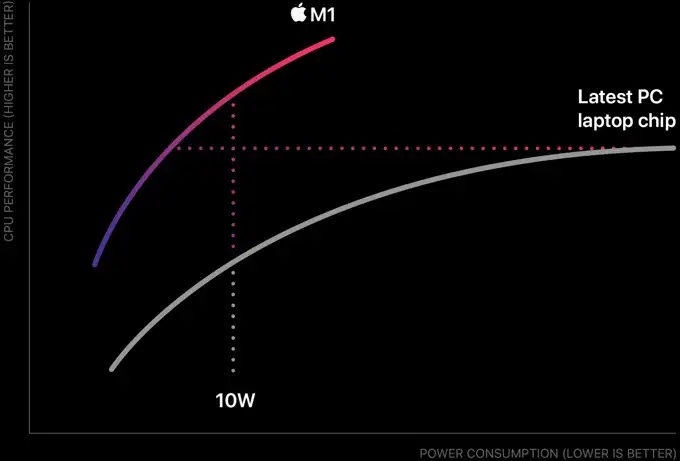
\includegraphics{./images/apple_graph.png}
\end{enumerate}

R offers a variety of packages for creating visually appealing and
informative plots. One of the most popular and versatile packages for
data visualization in R is \texttt{ggplot2}. We will explore the basics
of using \texttt{ggplot2} to create different types of plots and
customize them to suit your needs. We can load it separately
\texttt{libary(ggplot2)} or with \texttt{libary(tidyverse)}.

\hypertarget{grammar-of-graphics}{%
\section{Grammar of Graphics}\label{grammar-of-graphics}}

The Grammar of Graphics is a concept in data visualization that was
developed by Leland Wilkinson in his book ``The Grammar of Graphics''
(\emph{The Grammar of Graphics}
2005)\marginpar{\begin{footnotesize}\leavevmode\vadjust pre{\protect\hypertarget{ref-GrammarGraphics2005}{}}%
\emph{The Grammar of Graphics}. 2005. Statistics and Computing. New
York: Springer-Verlag. \url{https://doi.org/10.1007/0-387-28695-0}.\vspace{2mm}\par\end{footnotesize}}
in 1999. The Grammar of Graphics is essentially a system of rules that
describes how to represent data visually using a set of graphical
elements and mappings between data variables and visual properties.

``Excel Enjoyers'' are familiar with the Excel plotting workflow: you
select a plot you want and it just produces one for you.

\begin{figure}

{\centering 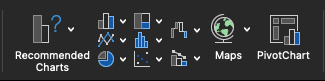
\includegraphics{./images/Excel_Plotting.png}

}

\caption{``Excel GUI''}

\end{figure}

Under this framework scatter plot and bar plots appear completely
different:

\begin{Shaded}
\begin{Highlighting}[]
\NormalTok{point\_plot }\OtherTok{\textless{}{-}}\NormalTok{ data\_raven }\SpecialCharTok{\%\textgreater{}\%} \FunctionTok{count}\NormalTok{(pr\_correct, }\AttributeTok{name =} \StringTok{"count"}\NormalTok{) }\SpecialCharTok{\%\textgreater{}\%} \FunctionTok{ggplot}\NormalTok{(}\FunctionTok{aes}\NormalTok{(}\AttributeTok{x =}\NormalTok{ pr\_correct, }\AttributeTok{y =}\NormalTok{ count)) }\SpecialCharTok{+} \FunctionTok{geom\_point}\NormalTok{(}\AttributeTok{size =} \DecValTok{3}\NormalTok{) }\SpecialCharTok{+} \FunctionTok{theme\_minimal}\NormalTok{()}
\NormalTok{col\_plot }\OtherTok{\textless{}{-}}\NormalTok{ data\_raven }\SpecialCharTok{\%\textgreater{}\%} \FunctionTok{count}\NormalTok{(pr\_correct, }\AttributeTok{name =} \StringTok{"count"}\NormalTok{) }\SpecialCharTok{\%\textgreater{}\%} \FunctionTok{ggplot}\NormalTok{(}\FunctionTok{aes}\NormalTok{(}\AttributeTok{x =}\NormalTok{ pr\_correct, }\AttributeTok{y =}\NormalTok{ count)) }\SpecialCharTok{+} \FunctionTok{geom\_col}\NormalTok{() }\SpecialCharTok{+} \FunctionTok{theme\_minimal}\NormalTok{()}
\NormalTok{point\_plot }\SpecialCharTok{+}\NormalTok{ col\_plot}
\end{Highlighting}
\end{Shaded}

\begin{figure}[H]

{\centering \includegraphics{./data_viz_files/figure-pdf/unnamed-chunk-4-1.pdf}

}

\end{figure}

However, under the Grammar of Graphics we see how similar these graphics
are! They are exactly the same in terms everything, but geometries! The
first one use ``points'' while the second uses ``columns'' to display
the data.

The Grammar of Graphics provides a framework for creating complex
visualizations by breaking down the visualization process into a set of
components.

\begin{figure}

{\centering 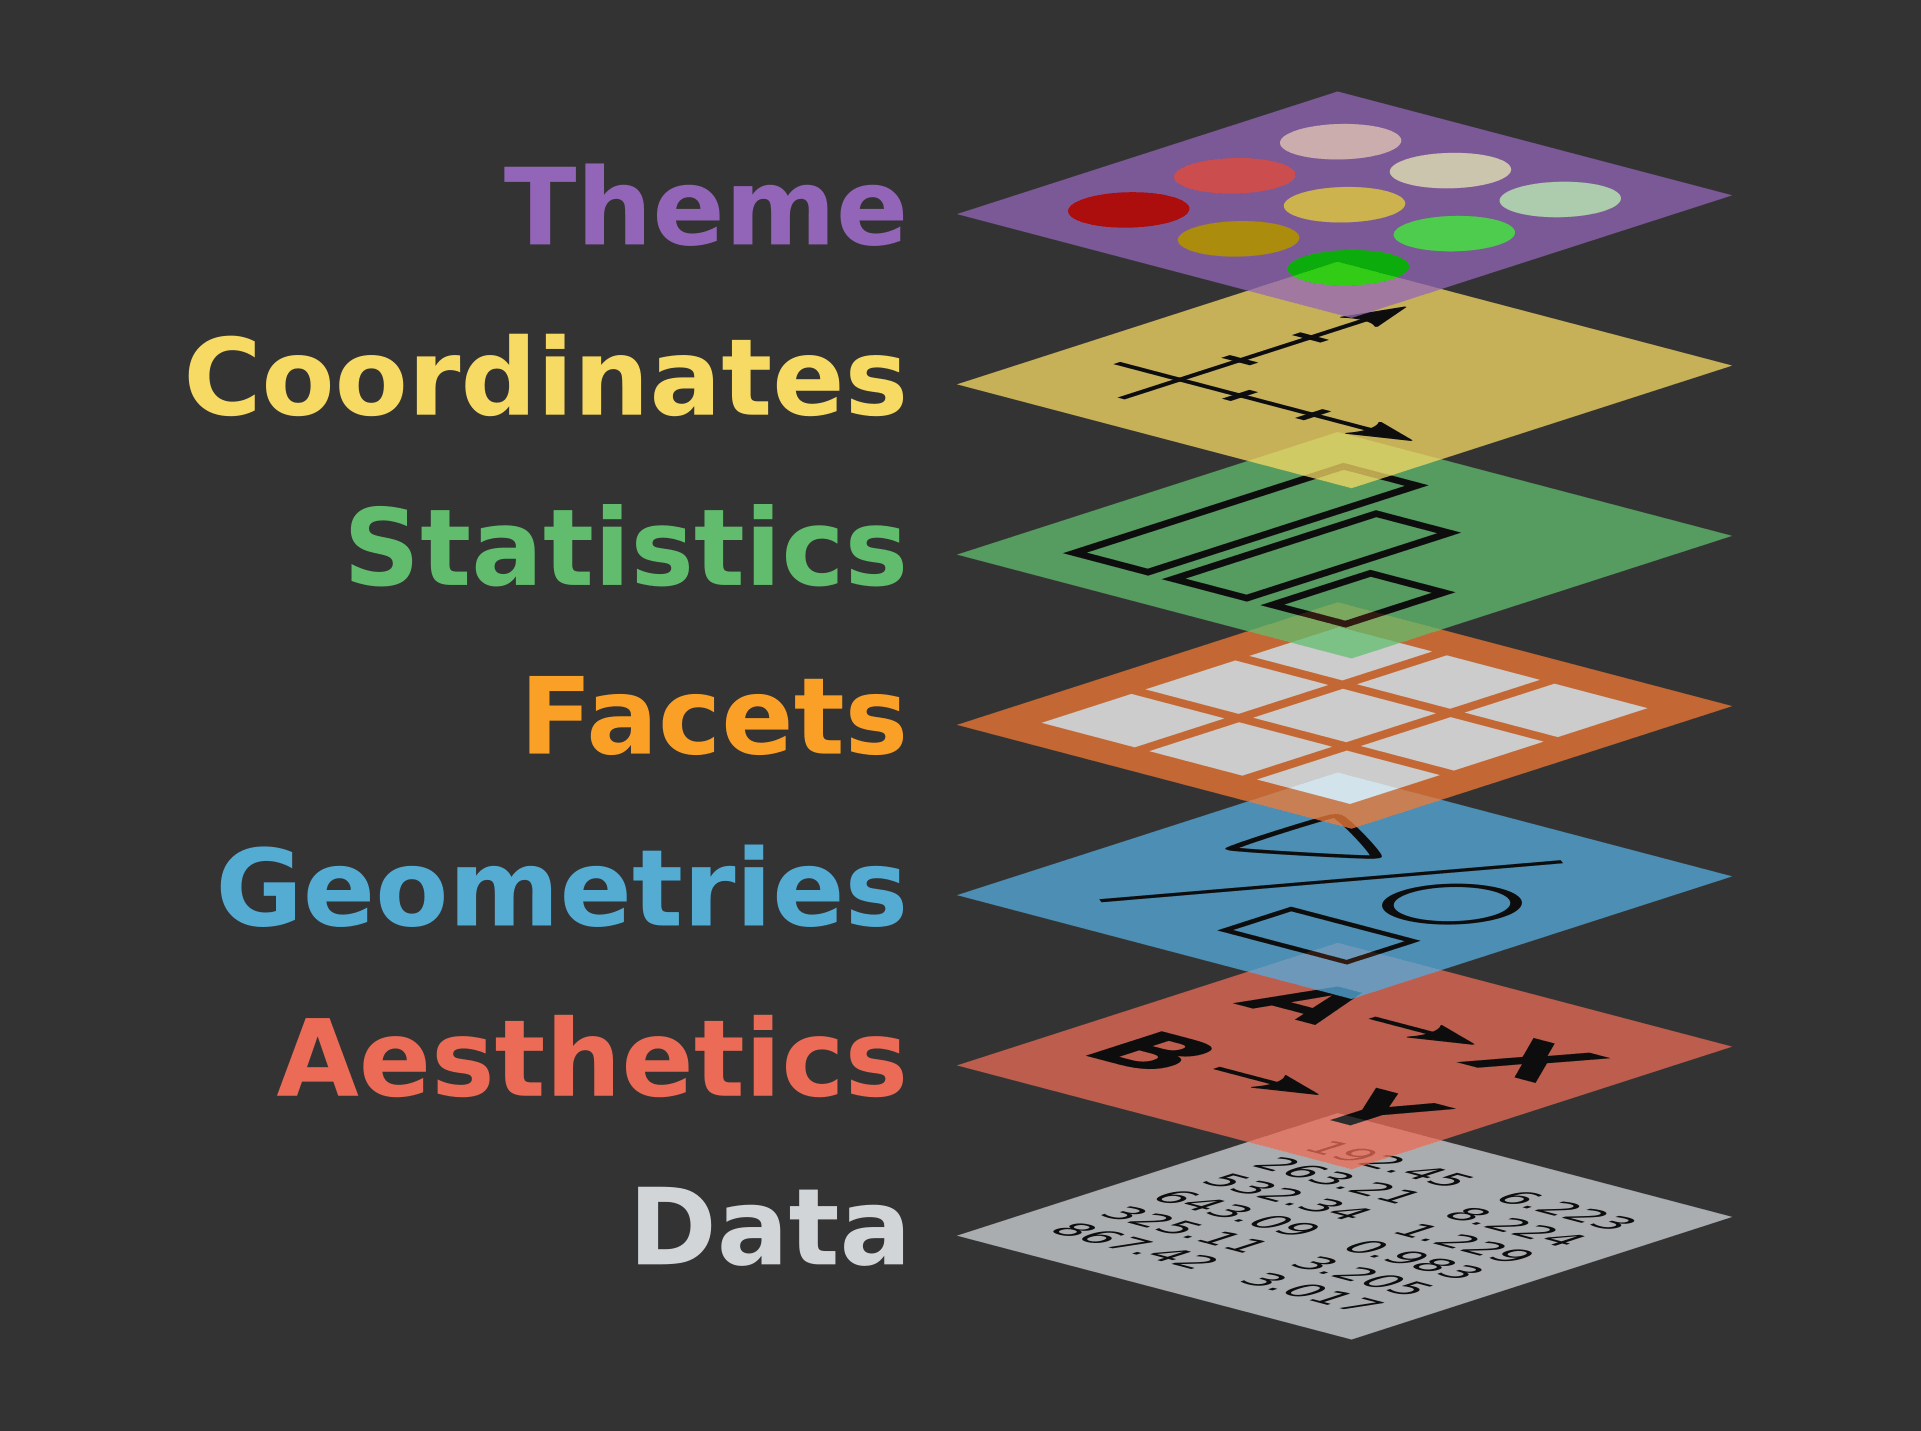
\includegraphics{./images/Grammar_of_Graphics.png}

}

\caption{``Grammar of Graphics Visual, from QCBS R Workshop 3''}

\end{figure}

\begin{enumerate}
\def\labelenumi{\arabic{enumi}.}
\tightlist
\item
  Data: The information that is being visualized. To explore how grammar
  of graphics works in \texttt{ggplot2} we will use \texttt{iris}
  dataset, which is a built-in dataset of measurements of different
  parts of iris flowers.
\end{enumerate}

\begin{verbatim}
  Sepal.Length Sepal.Width Petal.Length Petal.Width Species
1          5.1         3.5          1.4         0.2  setosa
2          4.9         3.0          1.4         0.2  setosa
3          4.7         3.2          1.3         0.2  setosa
4          4.6         3.1          1.5         0.2  setosa
5          5.0         3.6          1.4         0.2  setosa
6          5.4         3.9          1.7         0.4  setosa
\end{verbatim}

The Data layer of the graph is just a blank canvas. Becase we have not
specified any graphing elements yet.

\begin{Shaded}
\begin{Highlighting}[]
\NormalTok{data\_layer }\OtherTok{\textless{}{-}} \FunctionTok{ggplot}\NormalTok{(}\AttributeTok{data =}\NormalTok{ iris)}
\NormalTok{data\_layer}
\end{Highlighting}
\end{Shaded}

\begin{figure}[H]

{\centering 
\includegraphics{./data_viz_files/figure-pdf/unnamed-chunk-6-1.pdf}

}

\end{figure}

\begin{enumerate}
\def\labelenumi{\arabic{enumi}.}
\setcounter{enumi}{1}
\tightlist
\item
  Aesthetics: The visual properties used to represent the data, such as
  x, y, color or size. Once we add aethetics we see out plotting area
  being set up and if we check mapping we see that \texttt{Sepal.Length}
  was assigned to \texttt{x} and \texttt{Sepal.Width} was assigned to
  \texttt{y}.
\end{enumerate}

\begin{Shaded}
\begin{Highlighting}[]
\NormalTok{aes\_layer }\OtherTok{\textless{}{-}} \FunctionTok{ggplot}\NormalTok{(}\AttributeTok{data =}\NormalTok{ iris, }
                    \FunctionTok{aes}\NormalTok{(}\AttributeTok{x =}\NormalTok{ Sepal.Length, }\AttributeTok{y =}\NormalTok{ Sepal.Width)) }
\NormalTok{aes\_layer}
\end{Highlighting}
\end{Shaded}

\begin{figure}[H]

{\centering \includegraphics{./data_viz_files/figure-pdf/unnamed-chunk-7-1.pdf}

}

\end{figure}

\begin{Shaded}
\begin{Highlighting}[]
\NormalTok{aes\_layer}\SpecialCharTok{$}\NormalTok{mapping}
\end{Highlighting}
\end{Shaded}

\begin{verbatim}
Aesthetic mapping: 
* `x` -> `Sepal.Length`
* `y` -> `Sepal.Width`
\end{verbatim}

\begin{enumerate}
\def\labelenumi{\arabic{enumi}.}
\setcounter{enumi}{2}
\tightlist
\item
  Geometries: The visual elements used to represent the data, such as
  points or bars. Once we add geometry we start seeing our data!
\end{enumerate}

\begin{Shaded}
\begin{Highlighting}[]
\NormalTok{geometry\_layer }\OtherTok{\textless{}{-}}\NormalTok{ aes\_layer }\SpecialCharTok{+} \FunctionTok{geom\_point}\NormalTok{()}
\NormalTok{geometry\_layer}
\end{Highlighting}
\end{Shaded}

\begin{figure}[H]

{\centering \includegraphics{./data_viz_files/figure-pdf/unnamed-chunk-8-1.pdf}

}

\end{figure}

\begin{enumerate}
\def\labelenumi{\arabic{enumi}.}
\setcounter{enumi}{3}
\tightlist
\item
  Scales: The mapping between the data and the aesthetics, such as how
  numeric values are mapped to positions on a graph. There are different
  scales for color, fill, size, log(x), etc. Here we added scale
  \texttt{color}. Checking the mapping we see \texttt{Species} is mapped
  to \texttt{colour}.
\end{enumerate}

\begin{Shaded}
\begin{Highlighting}[]
\NormalTok{scales\_layer }\OtherTok{\textless{}{-}} \FunctionTok{ggplot}\NormalTok{(}\AttributeTok{data =}\NormalTok{ iris, }\FunctionTok{aes}\NormalTok{(}\AttributeTok{x =}\NormalTok{ Sepal.Length, }\AttributeTok{y =}\NormalTok{ Sepal.Width, }\AttributeTok{color =}\NormalTok{ Species)) }\SpecialCharTok{+}
  \FunctionTok{geom\_point}\NormalTok{() }\SpecialCharTok{+}
  \CommentTok{\# We case scale function to edit the scale for example we can set our own color manually}
  \FunctionTok{scale\_color\_manual}\NormalTok{(}\AttributeTok{values =} \FunctionTok{c}\NormalTok{(}\StringTok{"red"}\NormalTok{,}\StringTok{"orange"}\NormalTok{,}\StringTok{"pink"}\NormalTok{))}
\NormalTok{scales\_layer}
\end{Highlighting}
\end{Shaded}

\begin{figure}[H]

{\centering \includegraphics{./data_viz_files/figure-pdf/unnamed-chunk-9-1.pdf}

}

\end{figure}

\begin{Shaded}
\begin{Highlighting}[]
\NormalTok{scales\_layer}\SpecialCharTok{$}\NormalTok{mapping}
\end{Highlighting}
\end{Shaded}

\begin{verbatim}
Aesthetic mapping: 
* `x`      -> `Sepal.Length`
* `y`      -> `Sepal.Width`
* `colour` -> `Species`
\end{verbatim}

\begin{enumerate}
\def\labelenumi{\arabic{enumi}.}
\setcounter{enumi}{4}
\tightlist
\item
  Statistics: Mathematical transformations applied to the data before
  visualization, such as summary statistics or new variables. Histogram
  for example \emph{splits} data into bins and \emph{counts}
  observations.
\end{enumerate}

\begin{Shaded}
\begin{Highlighting}[]
\NormalTok{stat\_layer }\OtherTok{\textless{}{-}} \FunctionTok{ggplot}\NormalTok{(}\AttributeTok{data =}\NormalTok{ iris, }\FunctionTok{aes}\NormalTok{(}\AttributeTok{x =}\NormalTok{ Sepal.Length)) }\SpecialCharTok{+} 
  \FunctionTok{geom\_histogram}\NormalTok{(}\AttributeTok{bins =} \DecValTok{20}\NormalTok{, }\AttributeTok{color =} \StringTok{"white"}\NormalTok{)}
\NormalTok{stat\_layer}
\end{Highlighting}
\end{Shaded}

\begin{figure}[H]

{\centering \includegraphics{./data_viz_files/figure-pdf/unnamed-chunk-10-1.pdf}

}

\end{figure}

\begin{enumerate}
\def\labelenumi{\arabic{enumi}.}
\setcounter{enumi}{5}
\tightlist
\item
  Facets: Ways of dividing the data into subgroups and creating separate
  visualizations for each subgroup.
\end{enumerate}

\begin{Shaded}
\begin{Highlighting}[]
\NormalTok{facets\_layer }\OtherTok{\textless{}{-}}\NormalTok{ geometry\_layer }\SpecialCharTok{+} \FunctionTok{facet\_wrap}\NormalTok{(}\FunctionTok{vars}\NormalTok{(Species), }\AttributeTok{ncol =} \DecValTok{3}\NormalTok{) }
\NormalTok{facets\_layer}
\end{Highlighting}
\end{Shaded}

\begin{figure}[H]

{\centering \includegraphics{./data_viz_files/figure-pdf/unnamed-chunk-11-1.pdf}

}

\end{figure}

\begin{enumerate}
\def\labelenumi{\arabic{enumi}.}
\setcounter{enumi}{6}
\tightlist
\item
  Theme: Adding Polishing touches to your visual and making it look
  exactly the way you want.
\end{enumerate}

\begin{Shaded}
\begin{Highlighting}[]
\NormalTok{theme\_layer }\OtherTok{\textless{}{-}}\NormalTok{ facets\_layer }\SpecialCharTok{+} \FunctionTok{theme\_minimal}\NormalTok{(}\AttributeTok{base\_size =} \DecValTok{18}\NormalTok{) }\SpecialCharTok{+}  
  \FunctionTok{geom\_point}\NormalTok{(}\AttributeTok{size =} \DecValTok{2}\NormalTok{, }\AttributeTok{color =} \StringTok{"\#ffb86c"}\NormalTok{) }\SpecialCharTok{+}
  \FunctionTok{theme}\NormalTok{(}\AttributeTok{plot.background =} \FunctionTok{element\_rect}\NormalTok{(}\AttributeTok{fill =} \StringTok{"\#282a36"}\NormalTok{, }\AttributeTok{color =} \StringTok{"\#44475A"}\NormalTok{),}
        \AttributeTok{axis.text =} \FunctionTok{element\_text}\NormalTok{(}\AttributeTok{color =} \StringTok{"\#f8f8f2"}\NormalTok{),}
        \AttributeTok{axis.title =} \FunctionTok{element\_text}\NormalTok{(}\AttributeTok{color =} \StringTok{"\#f8f8f2"}\NormalTok{),}
        \AttributeTok{strip.text =} \FunctionTok{element\_text}\NormalTok{(}\AttributeTok{color =} \StringTok{"\#f8f8f2"}\NormalTok{),}
        \AttributeTok{panel.grid.minor =} \FunctionTok{element\_blank}\NormalTok{(),}
        \AttributeTok{panel.grid.major =} \FunctionTok{element\_line}\NormalTok{(}\AttributeTok{colour =} \StringTok{"\#44475a"}\NormalTok{)}
\NormalTok{        ) }\SpecialCharTok{+}
  \FunctionTok{labs}\NormalTok{(}\AttributeTok{x =} \StringTok{"Sepal Length"}\NormalTok{, }\AttributeTok{y =} \StringTok{"Sepal Width"}\NormalTok{)}
\NormalTok{theme\_layer}
\end{Highlighting}
\end{Shaded}

\begin{figure}[H]

{\centering 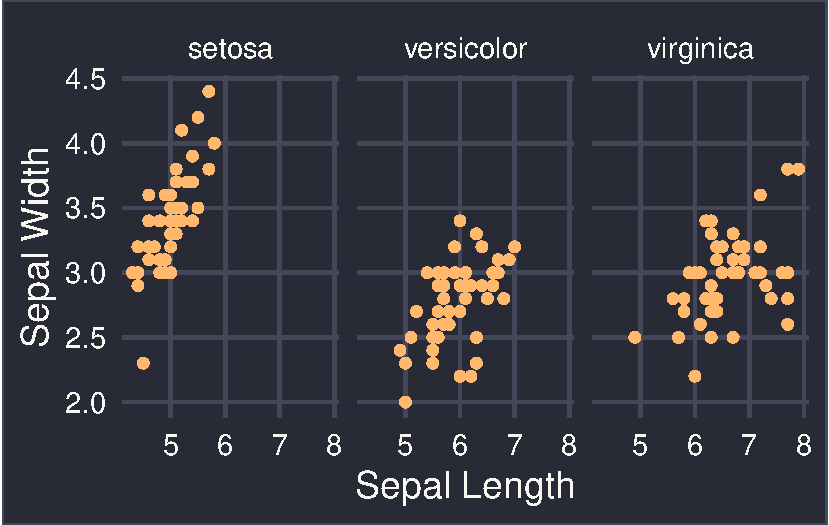
\includegraphics{./data_viz_files/figure-pdf/unnamed-chunk-12-1.pdf}

}

\end{figure}

\hypertarget{ggplot}{%
\section{\texorpdfstring{\texttt{ggplot()}}{ggplot()}}\label{ggplot}}

If you used R before then you are familiar with the default graphing
function \texttt{plot},\texttt{hist}, etc. \texttt{ggplot2} has it own
version of quickly making a graph \texttt{qplot()}. To learn about
\texttt{qplot()} check out
\href{http://www.sthda.com/english/wiki/qplot-quick-plot-with-ggplot2-r-software-and-data-visualization}{this
vignette}.

\begin{Shaded}
\begin{Highlighting}[]
\NormalTok{data\_raven }\SpecialCharTok{\%\textgreater{}\%} \FunctionTok{pull}\NormalTok{(pr\_correct) }\SpecialCharTok{\%\textgreater{}\%} \FunctionTok{hist}\NormalTok{() }
\end{Highlighting}
\end{Shaded}

\begin{figure}[H]

{\centering 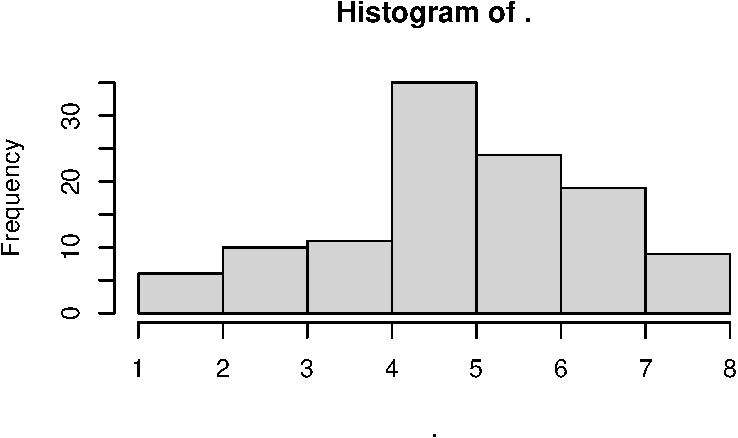
\includegraphics{./data_viz_files/figure-pdf/unnamed-chunk-13-1.pdf}

}

\end{figure}

\begin{Shaded}
\begin{Highlighting}[]
\NormalTok{data\_raven }\SpecialCharTok{\%\textgreater{}\%} \FunctionTok{qplot}\NormalTok{(pr\_correct, }\AttributeTok{data =}\NormalTok{ ., }\AttributeTok{geom =} \StringTok{\textquotesingle{}histogram\textquotesingle{}}\NormalTok{, }\AttributeTok{bins =} \FunctionTok{length}\NormalTok{(}\FunctionTok{unique}\NormalTok{(data\_raven}\SpecialCharTok{$}\NormalTok{pr\_correct)))}
\end{Highlighting}
\end{Shaded}

\begin{figure}[H]

{\centering 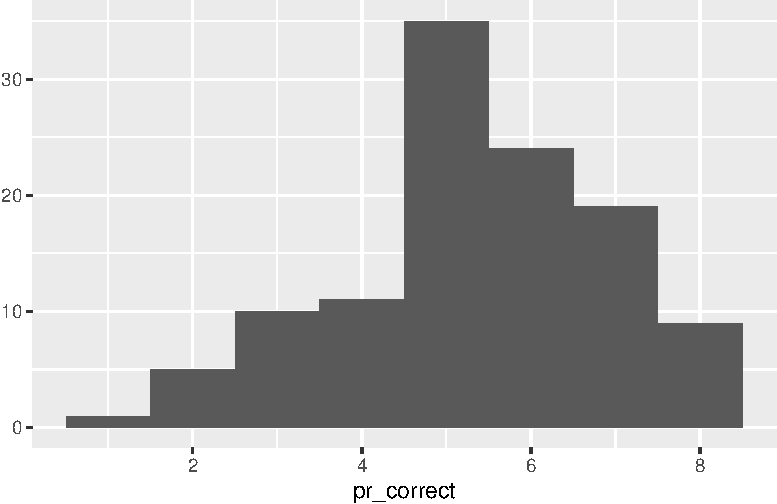
\includegraphics{./data_viz_files/figure-pdf/unnamed-chunk-13-2.pdf}

}

\end{figure}

The \texttt{ggplot()} function sets up the basic structure of a plot,
and additional layers, such as points, lines, and facets, can be added
using \texttt{+} operator (like \texttt{\%\textgreater{}\%}, but for
\texttt{+}). This makes it easy to understand, modify the code, and
build complex plots by adding layers. This allows for easy creation of
plots that reveal patterns in the data. In contrast, the basic R
plotting functions and \texttt{qplot()} have a simpler and less
expressive syntax, making it harder to create complex and multi-layered
plots. Mastering \texttt{ggplot()} is well worth your time and effort as
it will teach you how to think about graphs and what goes into building
them. For example, let's improve the histogram from earlier!

\begin{Shaded}
\begin{Highlighting}[]
\NormalTok{data\_raven }\SpecialCharTok{\%\textgreater{}\%} 
  \FunctionTok{count}\NormalTok{(pr\_correct) }\SpecialCharTok{\%\textgreater{}\%} \CommentTok{\# I prefer calculating statistics myself}
  \FunctionTok{ggplot}\NormalTok{(}\FunctionTok{aes}\NormalTok{(}\AttributeTok{x =} \FunctionTok{as.factor}\NormalTok{(pr\_correct), }\AttributeTok{y =}\NormalTok{ n)) }\SpecialCharTok{+} \CommentTok{\# We use aes to set x and y}
  \FunctionTok{geom\_col}\NormalTok{(}\AttributeTok{fill =} \StringTok{"steelblue"}\NormalTok{) }\SpecialCharTok{+}
  \FunctionTok{theme\_minimal}\NormalTok{(}\AttributeTok{base\_size =} \DecValTok{15}\NormalTok{) }\SpecialCharTok{+} 
  \FunctionTok{theme}\NormalTok{(}\AttributeTok{panel.grid =} \FunctionTok{element\_blank}\NormalTok{(), }
        \AttributeTok{panel.grid.major.y =} \FunctionTok{element\_line}\NormalTok{(}\AttributeTok{linewidth =} \FloatTok{0.5}\NormalTok{, }\AttributeTok{linetype =} \DecValTok{2}\NormalTok{, }\AttributeTok{color =} \StringTok{"grey"}\NormalTok{)) }\SpecialCharTok{+}
  \FunctionTok{labs}\NormalTok{(}\AttributeTok{x =} \StringTok{"Number of Correct Answers"}\NormalTok{, }
       \AttributeTok{y =} \StringTok{"Subject Count"}\NormalTok{, }
       \AttributeTok{title =} \StringTok{"Distribution of Correct Answers in Piece{-}rate Game"}\NormalTok{)}
\end{Highlighting}
\end{Shaded}

\begin{figure}[H]

{\centering \includegraphics{./data_viz_files/figure-pdf/unnamed-chunk-14-1.pdf}

}

\end{figure}

Ah much better! We added labels, removed unnecessary grid lines, and
added some color. If you want to learn more about ggplot check out
\href{https://ggplot2-book.org}{ggplot2: Elegant Graphics for Data
Analysis} (Hadley
2016)\marginpar{\begin{footnotesize}\leavevmode\vadjust pre{\protect\hypertarget{ref-hadleyGgplot22016}{}}%
Hadley, Wickham. 2016. \emph{Ggplot2}. New York, NY: Springer
Science+Business Media, LLC.\vspace{2mm}\par\end{footnotesize}}
and
\href{https://posit.co/wp-content/uploads/2022/10/data-visualization-1.pdf}{the
cheatsheet}.

We can use an amazing package \texttt{esquisse} to build our plots with
drag-and-drop!

\begin{Shaded}
\begin{Highlighting}[]
\CommentTok{\# install.packages(\textquotesingle{}esquisse\textquotesingle{})}
\FunctionTok{library}\NormalTok{(esquisse)}
\end{Highlighting}
\end{Shaded}

You can access \texttt{esquisse} by going to ``Addins'' in the top panel
or with \texttt{esquisser(your\_data)}. Now go learn more about this
package
\href{https://cran.r-project.org/web/packages/esquisse/vignettes/get-started.html}{here}.

\hypertarget{tips}{%
\section{Tips}\label{tips}}

\hypertarget{group}{%
\subsection{\texorpdfstring{\texttt{group}}{group}}\label{group}}

Usually ggplot groups your data by one the aesthetics you provided such
as \texttt{color} and \texttt{fill}; however, sometimes it fails to do
so. When that happens it is worth specifying group argument on your own.

Notice how labels for years 2020, 2021, 2022 are all over the place.

\begin{Shaded}
\begin{Highlighting}[]
\NormalTok{spending\_plot\_data }\SpecialCharTok{\%\textgreater{}\%} 
  \FunctionTok{ggplot}\NormalTok{(}\FunctionTok{aes}\NormalTok{(}\AttributeTok{x =}\NormalTok{ year, }\AttributeTok{y =}\NormalTok{ n, }\AttributeTok{fill =}\NormalTok{ agency, }\AttributeTok{label =}\NormalTok{ agency)) }\SpecialCharTok{+} 
  \FunctionTok{geom\_col}\NormalTok{(}\AttributeTok{position=}\StringTok{"fill"}\NormalTok{, }\AttributeTok{show.legend =}\NormalTok{ T) }\SpecialCharTok{+}
  \FunctionTok{scale\_fill\_manual}\NormalTok{( }
    \AttributeTok{values =} \FunctionTok{c}\NormalTok{(}\StringTok{"\#5E5E5E"}\NormalTok{, }\StringTok{"\#EF3B2C"}\NormalTok{, }\StringTok{"\#2CA25F"}\NormalTok{, }\StringTok{"\#006837"}\NormalTok{, }\StringTok{"\#F7DC6F"}\NormalTok{, }\StringTok{"\#00FFFF"}\NormalTok{, }\StringTok{"\#FFC0CB"}\NormalTok{)) }\SpecialCharTok{+}
  \FunctionTok{theme\_minimal}\NormalTok{() }\SpecialCharTok{+} 
  \FunctionTok{theme}\NormalTok{(}\AttributeTok{legend.position =} \StringTok{"none"}\NormalTok{) }\SpecialCharTok{+} 
  \FunctionTok{labs}\NormalTok{(}\AttributeTok{y =} \StringTok{"Millions Spent"}\NormalTok{, }\AttributeTok{fill =} \StringTok{"Department"}\NormalTok{) }\SpecialCharTok{+}
  \FunctionTok{geom\_label}\NormalTok{( }\AttributeTok{size =} \DecValTok{3}\NormalTok{, }\AttributeTok{position =} \FunctionTok{position\_fill}\NormalTok{(}\AttributeTok{vjust =} \FloatTok{0.5}\NormalTok{), }\AttributeTok{fill =} \StringTok{"white"}\NormalTok{, }\AttributeTok{alpha =} \FloatTok{0.5}\NormalTok{)}
\end{Highlighting}
\end{Shaded}

\begin{figure}[H]

{\centering 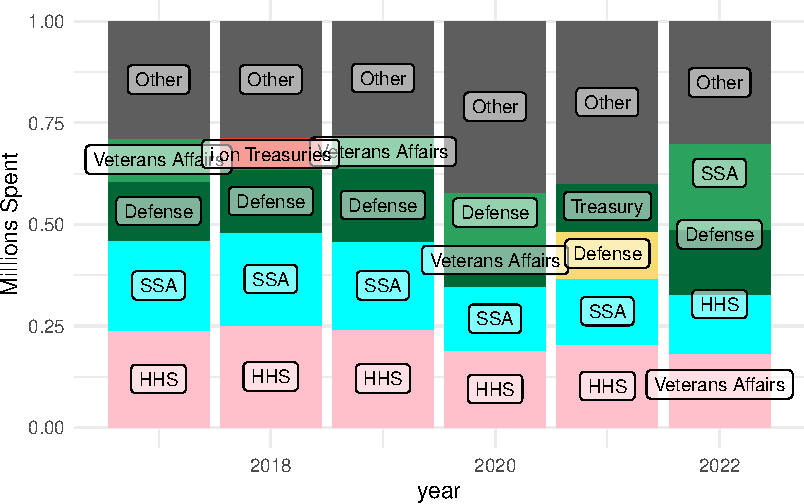
\includegraphics{./data_viz_files/figure-pdf/unnamed-chunk-17-1.pdf}

}

\end{figure}

If we specify group aesthetic everything goes back to its place!

\begin{Shaded}
\begin{Highlighting}[]
\NormalTok{spending\_plot\_data }\SpecialCharTok{\%\textgreater{}\%} 
  \FunctionTok{ggplot}\NormalTok{(}\FunctionTok{aes}\NormalTok{(}\AttributeTok{x =}\NormalTok{ year, }\AttributeTok{y =}\NormalTok{ n, }\AttributeTok{fill =}\NormalTok{ agency, }\AttributeTok{label =}\NormalTok{ agency)) }\SpecialCharTok{+} 
  \FunctionTok{geom\_col}\NormalTok{(}\AttributeTok{position=}\StringTok{"fill"}\NormalTok{, }\AttributeTok{show.legend =}\NormalTok{ T) }\SpecialCharTok{+}
  \FunctionTok{scale\_fill\_manual}\NormalTok{( }
    \AttributeTok{values =} \FunctionTok{c}\NormalTok{(}\StringTok{"\#5E5E5E"}\NormalTok{, }\StringTok{"\#EF3B2C"}\NormalTok{, }\StringTok{"\#2CA25F"}\NormalTok{, }\StringTok{"\#006837"}\NormalTok{, }\StringTok{"\#F7DC6F"}\NormalTok{, }\StringTok{"\#00FFFF"}\NormalTok{, }\StringTok{"\#FFC0CB"}\NormalTok{)) }\SpecialCharTok{+}
  \FunctionTok{theme\_minimal}\NormalTok{() }\SpecialCharTok{+} 
  \FunctionTok{theme}\NormalTok{(}\AttributeTok{legend.position =} \StringTok{"none"}\NormalTok{) }\SpecialCharTok{+} 
  \FunctionTok{labs}\NormalTok{(}\AttributeTok{y =} \StringTok{"Millions Spent"}\NormalTok{, }\AttributeTok{fill =} \StringTok{"Department"}\NormalTok{) }\SpecialCharTok{+}
  \FunctionTok{geom\_label}\NormalTok{( }\FunctionTok{aes}\NormalTok{(}\AttributeTok{group =}\NormalTok{ agency),}\AttributeTok{size =} \DecValTok{3}\NormalTok{, }\AttributeTok{position =} \FunctionTok{position\_fill}\NormalTok{(}\AttributeTok{vjust =} \FloatTok{0.5}\NormalTok{), }\AttributeTok{fill =} \StringTok{"white"}\NormalTok{, }\AttributeTok{alpha =} \FloatTok{0.5}\NormalTok{)}
\end{Highlighting}
\end{Shaded}

\begin{figure}[H]

{\centering 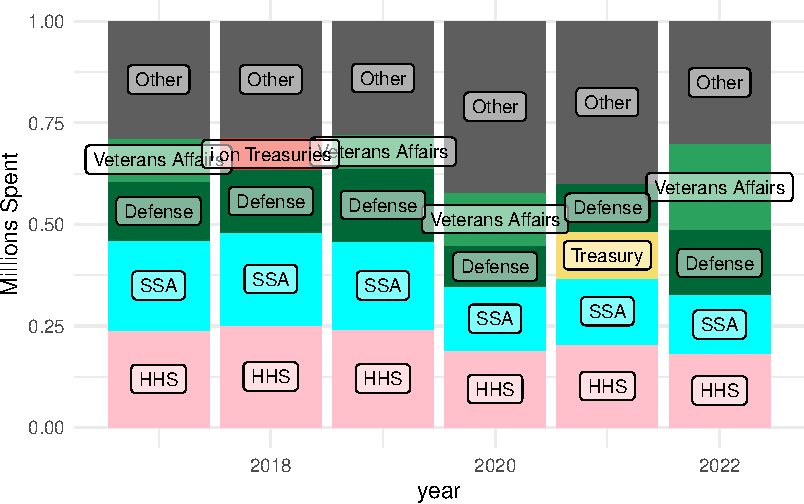
\includegraphics{./data_viz_files/figure-pdf/unnamed-chunk-18-1.pdf}

}

\end{figure}

This error is very common in line charts too.

\begin{Shaded}
\begin{Highlighting}[]
\NormalTok{group\_line\_data }\OtherTok{\textless{}{-}} \FunctionTok{tibble}\NormalTok{(}
 \AttributeTok{measure =} \FunctionTok{c}\NormalTok{(}\FunctionTok{rep}\NormalTok{(}\StringTok{"hot"}\NormalTok{,}\DecValTok{5}\NormalTok{),}\FunctionTok{rep}\NormalTok{(}\StringTok{"cool"}\NormalTok{,}\DecValTok{5}\NormalTok{)),}
 \AttributeTok{date =} \FunctionTok{rep}\NormalTok{(}\FunctionTok{seq}\NormalTok{(}\DecValTok{2000}\NormalTok{,}\DecValTok{2004}\NormalTok{, }\AttributeTok{by =} \DecValTok{1}\NormalTok{),}\DecValTok{2}\NormalTok{),}
 \AttributeTok{value =} \FunctionTok{c}\NormalTok{(}\DecValTok{89}\NormalTok{,}\DecValTok{111}\NormalTok{,}\DecValTok{100}\NormalTok{,}\DecValTok{130}\NormalTok{,}\DecValTok{159}\NormalTok{,}\DecValTok{24}\NormalTok{,}\DecValTok{37}\NormalTok{,}\DecValTok{88}\NormalTok{,}\DecValTok{69}\NormalTok{,}\DecValTok{105}\NormalTok{)}
\NormalTok{) }
\end{Highlighting}
\end{Shaded}

\begin{Shaded}
\begin{Highlighting}[]
\NormalTok{group\_line\_data }\SpecialCharTok{\%\textgreater{}\%} \FunctionTok{ggplot}\NormalTok{ (}\FunctionTok{aes}\NormalTok{(}\AttributeTok{x=}\NormalTok{date, }\AttributeTok{y=}\NormalTok{ value)) }\SpecialCharTok{+} \FunctionTok{geom\_line}\NormalTok{() }\SpecialCharTok{+} \FunctionTok{theme}\NormalTok{ (}\AttributeTok{legend.position =} \StringTok{"bottom"}\NormalTok{,}\AttributeTok{legend.title =} \FunctionTok{element\_blank}\NormalTok{()) }\SpecialCharTok{+} \FunctionTok{theme\_minimal}\NormalTok{()}
\end{Highlighting}
\end{Shaded}

\begin{figure}[H]

{\centering 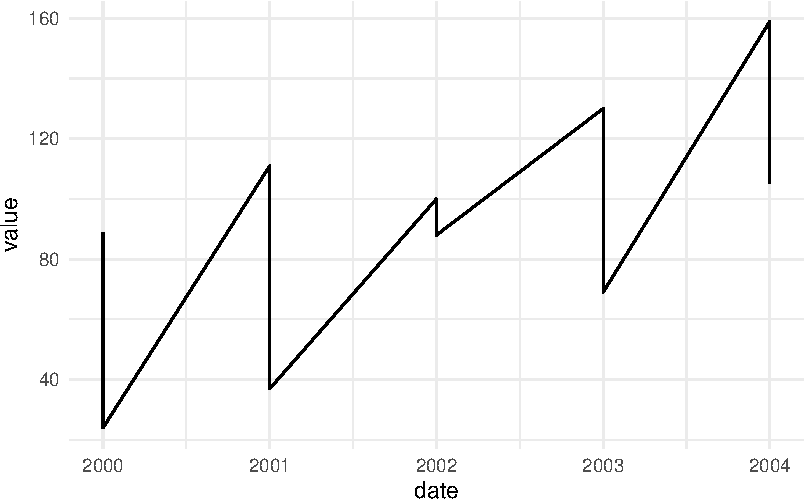
\includegraphics{./data_viz_files/figure-pdf/unnamed-chunk-20-1.pdf}

}

\end{figure}

\begin{Shaded}
\begin{Highlighting}[]
\NormalTok{group\_line\_data }\SpecialCharTok{\%\textgreater{}\%} \FunctionTok{ggplot}\NormalTok{ (}\FunctionTok{aes}\NormalTok{(}\AttributeTok{x=}\NormalTok{date, }\AttributeTok{y=}\NormalTok{ value, }\AttributeTok{group =}\NormalTok{ measure)) }\SpecialCharTok{+} \FunctionTok{geom\_line}\NormalTok{ () }\SpecialCharTok{+} \FunctionTok{theme}\NormalTok{ (}\AttributeTok{legend.position =} \StringTok{"bottom"}\NormalTok{,}\AttributeTok{legend.title =} \FunctionTok{element\_blank}\NormalTok{()) }\SpecialCharTok{+} \FunctionTok{theme\_minimal}\NormalTok{()}
\end{Highlighting}
\end{Shaded}

\begin{figure}[H]

{\centering 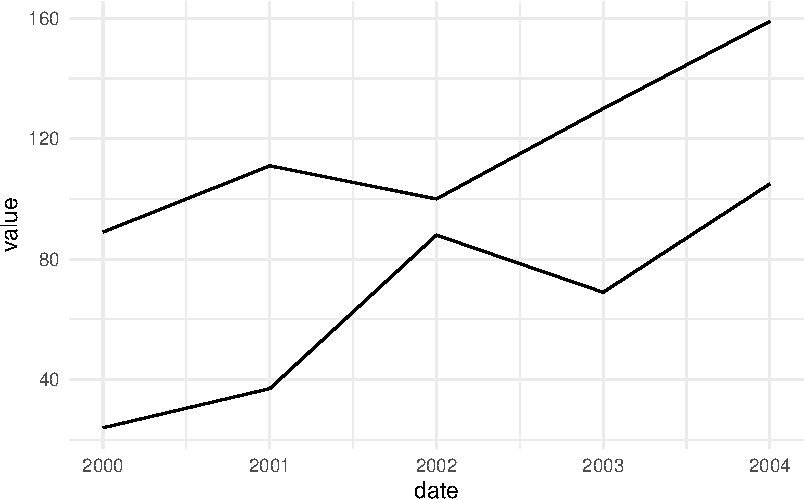
\includegraphics{./data_viz_files/figure-pdf/unnamed-chunk-20-2.pdf}

}

\end{figure}

\hypertarget{color}{%
\chapter{Color}\label{color}}

Color is a crucial component of data visualization. It has the power to
evoke emotions, highlight patterns, and communicate information that
might be difficult to convey through other means. Effective use of color
in data visualization can enhance the viewer's understanding and
engagement with the data, while poor use of color can obscure important
information and create confusion. We will learn how to easily create
different color schemes and palettes.

Color is a powerful tool because it can help convey information quickly
and effectively. By using different colors to represent different data
points or categories, we can create visual patterns that are easy to
interpret and remember. Color can also be used to highlight or draw
attention to important trends or outliers. Additionally, color can make
visualizations more engaging and appealing, which can help hold viewers'
attention and make them more likely to understand and remember the
information.

Color evokes responses that can influence people's emotions and
perception. Colors signify different emotions for example in the US red
is associated with danger or passion, blue with calmness or sadness, and
green with nature or health. Cultures have attached different meaning to
colors. So tailor color to your audience to elicit desired responses.
The effect of color is believed to be so powerful that locker room at
Iowa's Kinnick Stadium has been painted pink since 1979 with an idea to
lower opponent's testosterone levels.
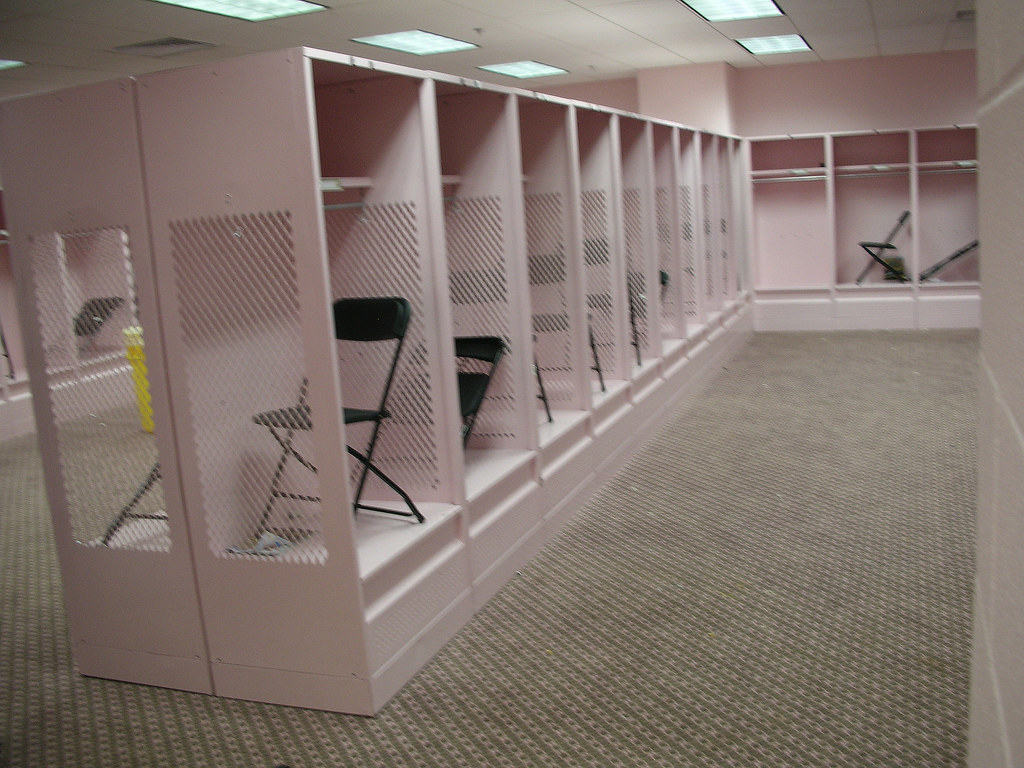
\includegraphics{./images/Kinnick_Stadium_Pink.jpeg}

\begin{figure}

{\centering 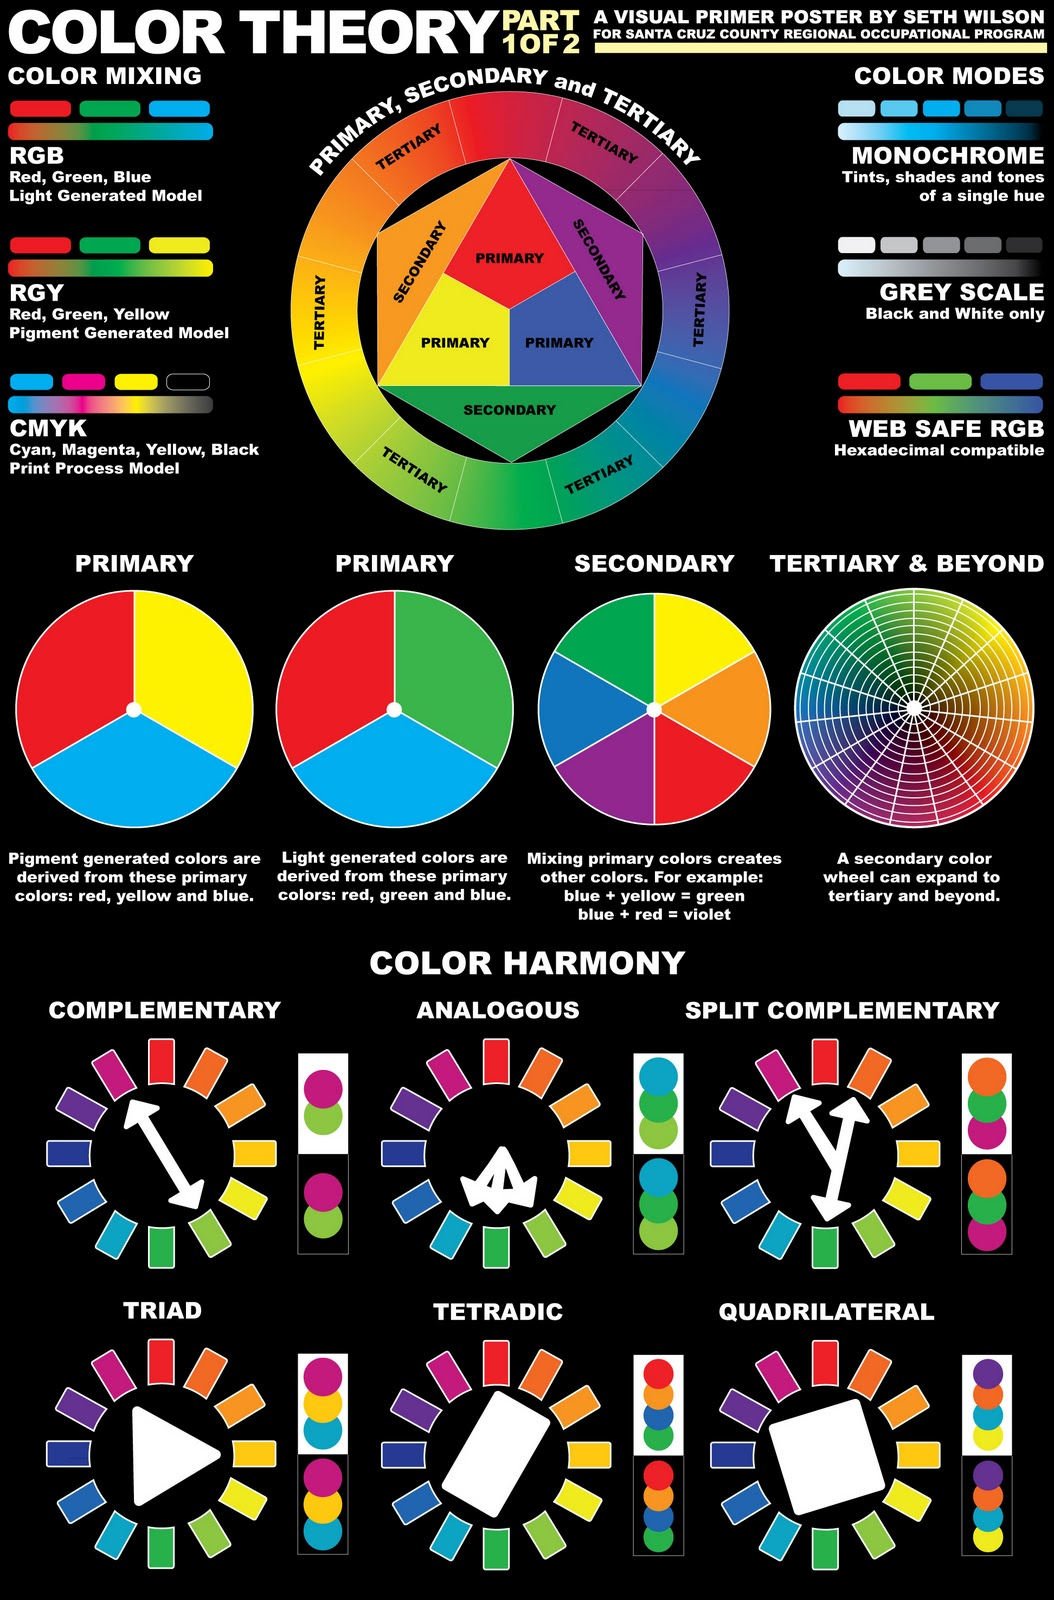
\includegraphics{./images/COLORTHEORY_A.jpeg}

}

\caption{color theory poster (Wilson
2011)\marginpar{\begin{footnotesize}\leavevmode\vadjust pre{\protect\hypertarget{ref-wilsonInkfumesPosterDesigns2011}{}}%
Wilson, Seth. 2011. {``Inkfumes: Poster Designs: Color, Design,
Typography Theory.''}
\url{http://inkfumes.blogspot.com/2011/10/poster-designs-color-design-typography.html}.\vspace{2mm}\par\end{footnotesize}}}

\end{figure}

\hypertarget{highlight-important-point}{%
\subsection{Highlight Important Point}\label{highlight-important-point}}

\begin{Shaded}
\begin{Highlighting}[]
\NormalTok{gapminder1997eu }\OtherTok{\textless{}{-}}\NormalTok{ gapminder }\SpecialCharTok{\%\textgreater{}\%} \FunctionTok{filter}\NormalTok{((year }\SpecialCharTok{==} \DecValTok{1997}\NormalTok{) }\SpecialCharTok{\&}\NormalTok{ (continent }\SpecialCharTok{==} \StringTok{"Europe"}\NormalTok{))}
\NormalTok{continents }\OtherTok{\textless{}{-}}\NormalTok{ gapminder }\SpecialCharTok{\%\textgreater{}\%} \FunctionTok{select}\NormalTok{(}\SpecialCharTok{{-}}\NormalTok{country) }\SpecialCharTok{\%\textgreater{}\%} \FunctionTok{mutate}\NormalTok{(}\AttributeTok{gdp =}\NormalTok{ gdpPercap }\SpecialCharTok{*}\NormalTok{ pop) }\SpecialCharTok{\%\textgreater{}\%} \FunctionTok{group\_by}\NormalTok{(year,continent) }\SpecialCharTok{\%\textgreater{}\%} \FunctionTok{summarize}\NormalTok{(}\AttributeTok{total\_pop\_mil =} \FunctionTok{sum}\NormalTok{(pop)}\SpecialCharTok{/}\DecValTok{10}\SpecialCharTok{\^{}}\DecValTok{6}\NormalTok{, }\AttributeTok{total\_gdp =} \FunctionTok{sum}\NormalTok{(gdp), }\AttributeTok{total\_gdppc =}\NormalTok{ total\_gdp}\SpecialCharTok{/}\NormalTok{(total\_pop\_mil}\SpecialCharTok{*}\DecValTok{10}\SpecialCharTok{\^{}}\DecValTok{6}\NormalTok{)) }\SpecialCharTok{\%\textgreater{}\%} \FunctionTok{ungroup}\NormalTok{()}
\NormalTok{malay\_miracle }\OtherTok{\textless{}{-}}\NormalTok{ gapminder }\SpecialCharTok{\%\textgreater{}\%} \FunctionTok{filter}\NormalTok{(country }\SpecialCharTok{\%in\%} \FunctionTok{c}\NormalTok{(}\StringTok{"Malaysia"}\NormalTok{, }\StringTok{"Vietnam"}\NormalTok{, }\StringTok{"Indonesia"}\NormalTok{, }\StringTok{"Thailand"}\NormalTok{))}
\NormalTok{asian\_tigers }\OtherTok{\textless{}{-}}\NormalTok{ gapminder }\SpecialCharTok{\%\textgreater{}\%} \FunctionTok{filter}\NormalTok{(country }\SpecialCharTok{\%in\%} \FunctionTok{c}\NormalTok{(}\StringTok{"Hong Kong, China"}\NormalTok{, }\StringTok{"Taiwan"}\NormalTok{, }\StringTok{"Singapore"}\NormalTok{, }\StringTok{"Korea, Rep."}\NormalTok{)) }\SpecialCharTok{\%\textgreater{}\%}
  \FunctionTok{mutate}\NormalTok{(}\AttributeTok{country =} \FunctionTok{recode}\NormalTok{(country,  }\StringTok{"Hong Kong, China"} \OtherTok{=} \StringTok{"Hong Kong"}\NormalTok{,  }\StringTok{"Korea, Rep."} \OtherTok{=} \StringTok{"South Korea"}\NormalTok{)) }
\end{Highlighting}
\end{Shaded}

We use color to emphasize certain data and give context. Below are
graphs comparing GDP of European Countries in 1997. First graph gives
each country its own color, creating a ``explosion at a candy factory''.
Second graph is an improvement as it removes the distraction, emphasizes
the country of the interest by highlighting ``Greece'' and greying out
the rest. The ``Red'' color signals that Greece might be doing not so
well.

\begin{Shaded}
\begin{Highlighting}[]
\NormalTok{p1 }\OtherTok{\textless{}{-}}\NormalTok{ gapminder1997eu }\SpecialCharTok{\%\textgreater{}\%} 
  \FunctionTok{mutate}\NormalTok{(}\AttributeTok{is.Greece =}\NormalTok{ country }\SpecialCharTok{==} \StringTok{"Greece"}\NormalTok{) }\SpecialCharTok{\%\textgreater{}\%}
  \FunctionTok{ggplot}\NormalTok{(}\FunctionTok{aes}\NormalTok{(}\AttributeTok{y =} \FunctionTok{fct\_reorder}\NormalTok{(country, gdpPercap), }\AttributeTok{x =}\NormalTok{ gdpPercap)) }\SpecialCharTok{+} 
  \FunctionTok{geom\_segment}\NormalTok{(}\FunctionTok{aes}\NormalTok{(}\AttributeTok{yend =}\NormalTok{ country, }\AttributeTok{xend=}\DecValTok{0}\NormalTok{, }\AttributeTok{color =}\NormalTok{ country), }\AttributeTok{size =} \DecValTok{1}\NormalTok{, }\AttributeTok{show.legend =} \ConstantTok{FALSE}\NormalTok{) }\SpecialCharTok{+}
  \FunctionTok{geom\_point}\NormalTok{(}\FunctionTok{aes}\NormalTok{(}\AttributeTok{color =}\NormalTok{ country), }\AttributeTok{show.legend =} \ConstantTok{FALSE}\NormalTok{, }\AttributeTok{size =} \DecValTok{3}\NormalTok{) }\SpecialCharTok{+} 
  \FunctionTok{theme\_minimal}\NormalTok{(}\AttributeTok{base\_size =} \DecValTok{12}\NormalTok{) }\SpecialCharTok{+} 
  \FunctionTok{theme}\NormalTok{(}\AttributeTok{panel.grid.major.y =} \FunctionTok{element\_blank}\NormalTok{(),}
        \AttributeTok{panel.grid.minor =} \FunctionTok{element\_blank}\NormalTok{()) }\SpecialCharTok{+}
 \CommentTok{\# ggplot2::scale\_color\_manual(values = c("\#7286D3","\#D37286")) +}
  \FunctionTok{labs}\NormalTok{(}\AttributeTok{x =} \StringTok{"GDP per Capita"}\NormalTok{, }\AttributeTok{y =} \FunctionTok{element\_blank}\NormalTok{()) }\SpecialCharTok{+} 
  \FunctionTok{coord\_cartesian}\NormalTok{(}\AttributeTok{expand =} \ConstantTok{FALSE}\NormalTok{, }\AttributeTok{clip =} \StringTok{\textquotesingle{}off\textquotesingle{}}\NormalTok{)}

\NormalTok{p2 }\OtherTok{\textless{}{-}}\NormalTok{ gapminder1997eu }\SpecialCharTok{\%\textgreater{}\%} 
  \FunctionTok{mutate}\NormalTok{(}\AttributeTok{is.Greece =}\NormalTok{ country }\SpecialCharTok{==} \StringTok{"Greece"}\NormalTok{) }\SpecialCharTok{\%\textgreater{}\%}
  \FunctionTok{ggplot}\NormalTok{(}\FunctionTok{aes}\NormalTok{(}\AttributeTok{y =} \FunctionTok{fct\_reorder}\NormalTok{(country, gdpPercap), }\AttributeTok{x =}\NormalTok{ gdpPercap)) }\SpecialCharTok{+} 
  \FunctionTok{geom\_segment}\NormalTok{(}\FunctionTok{aes}\NormalTok{(}\AttributeTok{yend =}\NormalTok{ country, }\AttributeTok{xend=}\DecValTok{0}\NormalTok{, }\AttributeTok{color =}\NormalTok{ is.Greece), }\AttributeTok{size =} \DecValTok{1}\NormalTok{, }\AttributeTok{show.legend =} \ConstantTok{FALSE}\NormalTok{) }\SpecialCharTok{+}
  \FunctionTok{geom\_point}\NormalTok{(}\FunctionTok{aes}\NormalTok{(}\AttributeTok{color =}\NormalTok{ is.Greece), }\AttributeTok{show.legend =} \ConstantTok{FALSE}\NormalTok{, }\AttributeTok{size =} \DecValTok{3}\NormalTok{) }\SpecialCharTok{+} 
  \FunctionTok{theme\_minimal}\NormalTok{(}\AttributeTok{base\_size =} \DecValTok{12}\NormalTok{) }\SpecialCharTok{+} 
  \FunctionTok{theme}\NormalTok{(}\AttributeTok{panel.grid.major.y =} \FunctionTok{element\_blank}\NormalTok{(),}
        \AttributeTok{panel.grid.minor =} \FunctionTok{element\_blank}\NormalTok{()) }\SpecialCharTok{+}
\NormalTok{  ggplot2}\SpecialCharTok{::}\FunctionTok{scale\_color\_manual}\NormalTok{(}\AttributeTok{values =} \FunctionTok{c}\NormalTok{(}\StringTok{"grey"}\NormalTok{,}\StringTok{"\#D37286"}\NormalTok{)) }\SpecialCharTok{+}
  \FunctionTok{labs}\NormalTok{(}\AttributeTok{x =} \StringTok{"GDP per Capita"}\NormalTok{, }\AttributeTok{y =} \FunctionTok{element\_blank}\NormalTok{()) }\SpecialCharTok{+} 
  \FunctionTok{coord\_cartesian}\NormalTok{(}\AttributeTok{expand =} \ConstantTok{FALSE}\NormalTok{, }\AttributeTok{clip =} \StringTok{\textquotesingle{}off\textquotesingle{}}\NormalTok{)}

\NormalTok{p1 }\SpecialCharTok{+}\NormalTok{ p2 }\SpecialCharTok{+} \FunctionTok{plot\_annotation}\NormalTok{(}\AttributeTok{title =} \StringTok{"Countries in Europe by GDP per Capita"}\NormalTok{,}\AttributeTok{theme =} \FunctionTok{theme}\NormalTok{(}\AttributeTok{plot.title =} \FunctionTok{element\_text}\NormalTok{(}\AttributeTok{size =} \DecValTok{16}\NormalTok{)))}
\end{Highlighting}
\end{Shaded}

\begin{figure}[H]

{\centering \includegraphics{./color_files/figure-pdf/unnamed-chunk-3-1.pdf}

}

\end{figure}

\hypertarget{comparing-two-things}{%
\subsection{Comparing Two Things}\label{comparing-two-things}}

\hypertarget{complementary-harmony-with-a-positivenegative-connotation}{%
\subsubsection{Complementary Harmony with a Positive/Negative
Connotation}\label{complementary-harmony-with-a-positivenegative-connotation}}

Complementary Harmony refers to the use of colors that are opposite each
other on the color wheel to create a strong contrast. This creates a
positive/negative connotation that is good for showcasing differences.
Colors near each other on the wheel can also work well together, but
opposite colors provide the strongest support for a key color. The
example below shows the comparison between population of Asia and
Europe. The use of bright purple emphasizes the outstanding population
growth of Asia, while the green color highlights the slower population
growth in Europe.

\begin{Shaded}
\begin{Highlighting}[]
\NormalTok{p3 }\OtherTok{\textless{}{-}}\NormalTok{ continents }\SpecialCharTok{\%\textgreater{}\%} 
  \FunctionTok{filter}\NormalTok{(continent }\SpecialCharTok{\%in\%} \FunctionTok{c}\NormalTok{(}\StringTok{"Asia"}\NormalTok{,}\StringTok{"Europe"}\NormalTok{)) }\SpecialCharTok{\%\textgreater{}\%} 
  \FunctionTok{ggplot}\NormalTok{(}\FunctionTok{aes}\NormalTok{(}\AttributeTok{x=}\NormalTok{year, }\AttributeTok{y =}\NormalTok{ total\_pop\_mil, }\AttributeTok{color =}\NormalTok{ continent)) }\SpecialCharTok{+} 
  \FunctionTok{geom\_line}\NormalTok{(}\AttributeTok{linewidth =} \FloatTok{1.5}\NormalTok{) }\SpecialCharTok{+} 
  \FunctionTok{theme\_minimal}\NormalTok{() }\SpecialCharTok{+} 
  \FunctionTok{theme}\NormalTok{(}\AttributeTok{legend.position =} \StringTok{"none"}\NormalTok{) }\SpecialCharTok{+}
  \FunctionTok{scale\_y\_log10}\NormalTok{() }\SpecialCharTok{+} 
  \FunctionTok{scale\_color\_manual}\NormalTok{(}\AttributeTok{values =} \FunctionTok{c}\NormalTok{(}\StringTok{"\#DA70D6"}\NormalTok{, }\StringTok{"\#70DA74"}\NormalTok{)) }\SpecialCharTok{+}
  \FunctionTok{geom\_dl}\NormalTok{(}\FunctionTok{aes}\NormalTok{(}\AttributeTok{label =}\NormalTok{ continent), }\AttributeTok{method =} \StringTok{"smart.grid"}\NormalTok{) }\SpecialCharTok{+}
  \FunctionTok{labs}\NormalTok{(}\AttributeTok{x =} \FunctionTok{element\_blank}\NormalTok{(), }\AttributeTok{y =} \StringTok{"Population in Millions (log10)"}\NormalTok{)}
  

\NormalTok{complementary }\SpecialCharTok{+}\NormalTok{ p3 }\SpecialCharTok{+} \FunctionTok{plot\_annotation}\NormalTok{(}\AttributeTok{title =} \StringTok{"Complementary Harmony with a Positive/Negative Connotation"}\NormalTok{, }\AttributeTok{theme =} \FunctionTok{theme}\NormalTok{(}\AttributeTok{plot.title =} \FunctionTok{element\_text}\NormalTok{(}\AttributeTok{size =} \DecValTok{16}\NormalTok{)))}
\end{Highlighting}
\end{Shaded}

\begin{figure}[H]

{\centering \includegraphics{./color_files/figure-pdf/unnamed-chunk-5-1.pdf}

}

\end{figure}

\hypertarget{near-complementary-harmony-for-highlighting-two-series-where-one-is-the-primary-focus}{%
\subsubsection{Near Complementary Harmony for Highlighting Two Series
Where One Is the Primary
Focus}\label{near-complementary-harmony-for-highlighting-two-series-where-one-is-the-primary-focus}}

Near Complementary Harmony is a color scheme that creates good contrast
without using polar opposite colors. It involves selecting a color that
is 33\% around the color wheel from the key color instead of the full
50\%. This works well for highlighting two series where one is the
primary focus. It is best to use warm colors for the key color and cool
colors for the complementary colors. If necessary, the complementary
colors can be muted by decreasing their saturation or altering their
lightness to reduce the contrast with the background. The example below
highlights the importance of population growth in Asia, with Europe
being presented neutrally as a point of comparison rather than as a
slow-growing region.

\begin{Shaded}
\begin{Highlighting}[]
\NormalTok{p4 }\OtherTok{\textless{}{-}}\NormalTok{ continents }\SpecialCharTok{\%\textgreater{}\%} 
  \FunctionTok{filter}\NormalTok{(continent }\SpecialCharTok{\%in\%} \FunctionTok{c}\NormalTok{(}\StringTok{"Asia"}\NormalTok{,}\StringTok{"Europe"}\NormalTok{)) }\SpecialCharTok{\%\textgreater{}\%} 
  \FunctionTok{ggplot}\NormalTok{(}\FunctionTok{aes}\NormalTok{(}\AttributeTok{x=}\NormalTok{year, }\AttributeTok{y =}\NormalTok{ total\_pop\_mil, }\AttributeTok{color =}\NormalTok{ continent)) }\SpecialCharTok{+} 
  \FunctionTok{geom\_line}\NormalTok{(}\AttributeTok{size =} \FloatTok{1.5}\NormalTok{) }\SpecialCharTok{+} 
  \FunctionTok{theme\_minimal}\NormalTok{() }\SpecialCharTok{+} 
  \FunctionTok{theme}\NormalTok{(}\AttributeTok{legend.position =} \StringTok{"none"}\NormalTok{) }\SpecialCharTok{+}
  \FunctionTok{scale\_y\_log10}\NormalTok{() }\SpecialCharTok{+}
  \FunctionTok{scale\_color\_manual}\NormalTok{(}\AttributeTok{values =} \FunctionTok{c}\NormalTok{(}\StringTok{"\#DA70D6"}\NormalTok{, }\StringTok{"\#70D6DA"}\NormalTok{))  }\SpecialCharTok{+}
  \FunctionTok{geom\_dl}\NormalTok{(}\FunctionTok{aes}\NormalTok{(}\AttributeTok{label =}\NormalTok{ continent), }\AttributeTok{method =} \StringTok{"smart.grid"}\NormalTok{) }\SpecialCharTok{+}
  \FunctionTok{labs}\NormalTok{(}\AttributeTok{x =} \FunctionTok{element\_blank}\NormalTok{(), }\AttributeTok{y =} \StringTok{"Population in Millions (log10)"}\NormalTok{)}

\NormalTok{triadic }\SpecialCharTok{+}\NormalTok{ p4 }\SpecialCharTok{+} \FunctionTok{plot\_annotation}\NormalTok{(}\AttributeTok{title =} \StringTok{"Near Complementary Harmony for Highlighting }\SpecialCharTok{\textbackslash{}n}\StringTok{Two Series Where One Is the Primary Focus"}\NormalTok{,}\AttributeTok{theme =} \FunctionTok{theme}\NormalTok{(}\AttributeTok{plot.title =} \FunctionTok{element\_text}\NormalTok{(}\AttributeTok{size =} \DecValTok{16}\NormalTok{)))}
\end{Highlighting}
\end{Shaded}

\begin{figure}[H]

{\centering 
\includegraphics{./color_files/figure-pdf/unnamed-chunk-6-1.pdf}

}

\end{figure}

\hypertarget{color-palettes-for-comparing-three-things}{%
\subsection{Color Palettes for Comparing Three
Things}\label{color-palettes-for-comparing-three-things}}

\hypertarget{analogoustriadic-harmony-for-highlighting-three-series}{%
\subsubsection{Analogous/Triadic Harmony for Highlighting Three
Series}\label{analogoustriadic-harmony-for-highlighting-three-series}}

Analogous harmony involves using neighboring colors to the key color for
simple distinctions among categories. In contrast, triadic harmony uses
the key color and two complementary colors evenly spaced around the
color wheel for greater contrast, but may lose the emphasis on the key
color. The example below displays the population of three countries
without any specific emphasis.

\begin{Shaded}
\begin{Highlighting}[]
\NormalTok{p5 }\OtherTok{\textless{}{-}}\NormalTok{ continents }\SpecialCharTok{\%\textgreater{}\%} 
  \FunctionTok{filter}\NormalTok{(continent }\SpecialCharTok{\%in\%} \FunctionTok{c}\NormalTok{(}\StringTok{"Asia"}\NormalTok{,}\StringTok{"Europe"}\NormalTok{,}\StringTok{"Americas"}\NormalTok{)) }\SpecialCharTok{\%\textgreater{}\%} 
  \FunctionTok{ggplot}\NormalTok{(}\FunctionTok{aes}\NormalTok{(}\AttributeTok{x=}\NormalTok{year, }\AttributeTok{y =}\NormalTok{ total\_pop\_mil, }\AttributeTok{color =}\NormalTok{ continent)) }\SpecialCharTok{+} 
  \FunctionTok{geom\_line}\NormalTok{(}\AttributeTok{size =} \FloatTok{1.5}\NormalTok{) }\SpecialCharTok{+} 
  \FunctionTok{theme\_minimal}\NormalTok{() }\SpecialCharTok{+} 
  \FunctionTok{theme}\NormalTok{(}\AttributeTok{legend.position =} \StringTok{"none"}\NormalTok{) }\SpecialCharTok{+}
  \FunctionTok{scale\_y\_log10}\NormalTok{() }\SpecialCharTok{+}
  \FunctionTok{scale\_color\_manual}\NormalTok{(}\AttributeTok{values =} \FunctionTok{c}\NormalTok{(}\StringTok{"\#DA70D6"}\NormalTok{, }\StringTok{"\#DA70A1"}\NormalTok{, }\StringTok{"\#A970DA"}\NormalTok{))  }\SpecialCharTok{+}
  \FunctionTok{geom\_dl}\NormalTok{(}\FunctionTok{aes}\NormalTok{(}\AttributeTok{label =}\NormalTok{ continent), }\AttributeTok{method =} \StringTok{"smart.grid"}\NormalTok{) }\SpecialCharTok{+}
  \FunctionTok{labs}\NormalTok{(}\AttributeTok{x =} \FunctionTok{element\_blank}\NormalTok{(), }\AttributeTok{y =} \StringTok{"Population in Millions (log10)"}\NormalTok{)}

\NormalTok{analogous }\SpecialCharTok{+}\NormalTok{ p5 }\SpecialCharTok{+} \FunctionTok{plot\_annotation}\NormalTok{(}\AttributeTok{title =} \StringTok{"Analogous/Triadic Harmony for Highlighting Three Series"}\NormalTok{,}\AttributeTok{theme =} \FunctionTok{theme}\NormalTok{(}\AttributeTok{plot.title =} \FunctionTok{element\_text}\NormalTok{(}\AttributeTok{size =} \DecValTok{16}\NormalTok{)))}
\end{Highlighting}
\end{Shaded}

\begin{figure}[H]

{\centering \includegraphics{./color_files/figure-pdf/unnamed-chunk-7-1.pdf}

}

\end{figure}

\hypertarget{highlighting-one-series-against-two-related-series}{%
\subsubsection{Highlighting One Series Against Two Related
Series}\label{highlighting-one-series-against-two-related-series}}

Near Complementary Harmony is a color scheme that creates good contrast
without using polar opposite colors. It involves selecting a color that
is 33\% around the color wheel from the key color instead of the full
50\%. This works well for highlighting two series where one is the
primary focus. It is best to use warm colors for the key color and cool
colors for the complementary colors. If necessary, the complementary
colors can be muted by decreasing their saturation or altering their
lightness to reduce the contrast with the background. The example below
highlights the GDPs of 3 countries with emphasis on Asia through the use
of the purple color. Europe and the Americas are depicted with similar
shades of green, indicating their lesser significance for the narrative.

\begin{Shaded}
\begin{Highlighting}[]
\NormalTok{p6 }\OtherTok{\textless{}{-}}\NormalTok{ continents }\SpecialCharTok{\%\textgreater{}\%} 
  \FunctionTok{filter}\NormalTok{(continent }\SpecialCharTok{\%in\%} \FunctionTok{c}\NormalTok{(}\StringTok{"Asia"}\NormalTok{,}\StringTok{"Europe"}\NormalTok{,}\StringTok{"Americas"}\NormalTok{)) }\SpecialCharTok{\%\textgreater{}\%} 
  \FunctionTok{ggplot}\NormalTok{(}\FunctionTok{aes}\NormalTok{(}\AttributeTok{x=}\NormalTok{year, }\AttributeTok{y =}\NormalTok{ total\_gdppc, }\AttributeTok{color =}\NormalTok{ continent)) }\SpecialCharTok{+} 
  \FunctionTok{geom\_line}\NormalTok{(}\AttributeTok{size =} \FloatTok{1.5}\NormalTok{) }\SpecialCharTok{+} 
  \FunctionTok{theme\_minimal}\NormalTok{() }\SpecialCharTok{+} 
  \FunctionTok{theme}\NormalTok{(}\AttributeTok{legend.position =} \StringTok{"none"}\NormalTok{) }\SpecialCharTok{+}
  \FunctionTok{scale\_y\_log10}\NormalTok{() }\SpecialCharTok{+}
  \FunctionTok{scale\_color\_manual}\NormalTok{(}\AttributeTok{values =} \FunctionTok{c}\NormalTok{( }\StringTok{"\#A1DA70"}\NormalTok{, }\StringTok{"\#DA70D6"}\NormalTok{, }\StringTok{"\#70DAA9"}\NormalTok{)) }\SpecialCharTok{+}
  \FunctionTok{geom\_dl}\NormalTok{(}\FunctionTok{aes}\NormalTok{(}\AttributeTok{label =}\NormalTok{ continent), }\AttributeTok{method =} \StringTok{"smart.grid"}\NormalTok{) }\SpecialCharTok{+}
  \FunctionTok{labs}\NormalTok{(}\AttributeTok{x =} \FunctionTok{element\_blank}\NormalTok{(), }\AttributeTok{y =} \StringTok{"GDP per Capita (log10)"}\NormalTok{)}

\NormalTok{complementary\_3 }\SpecialCharTok{+}\NormalTok{ p6 }\SpecialCharTok{+} \FunctionTok{plot\_annotation}\NormalTok{(}\AttributeTok{title =} \StringTok{"Highlighting One Series Against Two Related Series"}\NormalTok{,}\AttributeTok{theme =} \FunctionTok{theme}\NormalTok{(}\AttributeTok{plot.title =} \FunctionTok{element\_text}\NormalTok{(}\AttributeTok{size =} \DecValTok{16}\NormalTok{)))}
\end{Highlighting}
\end{Shaded}

\begin{figure}[H]

{\centering \includegraphics{./color_files/figure-pdf/unnamed-chunk-8-1.pdf}

}

\end{figure}

\hypertarget{color-palettes-for-comparing-four-things}{%
\subsection{Color Palettes for Comparing Four
Things}\label{color-palettes-for-comparing-four-things}}

\hypertarget{analogous-complementary-for-one-main-series-and-its-three-secondary}{%
\subsubsection{Analogous Complementary for One Main Series and Its Three
Secondary}\label{analogous-complementary-for-one-main-series-and-its-three-secondary}}

Analogous Complementary is a color scheme that uses four colors, where
the key color and its complementary color are combined with two colors
that are one step away from the complementary color. This scheme still
allows for analogous harmony while creating a quartet of colors that can
be used for one main series and its three components. The similarities
between the three complementary colors make the key color stand out. The
example below shows Malaysian Economic Miracle in comparison to
Malaysia's three neighbors.

\begin{Shaded}
\begin{Highlighting}[]
\NormalTok{p7 }\OtherTok{\textless{}{-}}\NormalTok{ malay\_miracle }\SpecialCharTok{\%\textgreater{}\%} \FunctionTok{ggplot}\NormalTok{(}\FunctionTok{aes}\NormalTok{(}\AttributeTok{x =}\NormalTok{ year, }\AttributeTok{y =}\NormalTok{ gdpPercap, }\AttributeTok{color =}\NormalTok{ country)) }\SpecialCharTok{+} 
  \FunctionTok{geom\_line}\NormalTok{(}\AttributeTok{linewidth =} \FloatTok{1.5}\NormalTok{) }\SpecialCharTok{+} 
  \FunctionTok{theme\_minimal}\NormalTok{() }\SpecialCharTok{+} 
  \CommentTok{\#scale\_y\_log10() +}
  \FunctionTok{theme}\NormalTok{(}\AttributeTok{legend.position =} \StringTok{"none"}\NormalTok{) }\SpecialCharTok{+}
  \FunctionTok{scale\_color\_manual}\NormalTok{(}\AttributeTok{values =} \FunctionTok{c}\NormalTok{(}\StringTok{"\#A1DA70"}\NormalTok{, }\StringTok{"\#DA70D6"}\NormalTok{, }\StringTok{"\#70DA74"}\NormalTok{, }\StringTok{"\#70DAA9"}\NormalTok{)) }\SpecialCharTok{+}
  \FunctionTok{geom\_dl}\NormalTok{(}\FunctionTok{aes}\NormalTok{(}\AttributeTok{label =}\NormalTok{ country), }\AttributeTok{method =} \StringTok{"smart.grid"}\NormalTok{) }\SpecialCharTok{+}
  \FunctionTok{labs}\NormalTok{(}\AttributeTok{x =} \FunctionTok{element\_blank}\NormalTok{(), }\AttributeTok{y =} \StringTok{"GDP per Capita (log10)"}\NormalTok{)}

\NormalTok{complementary\_4 }\SpecialCharTok{+}\NormalTok{ p7 }\SpecialCharTok{+} \FunctionTok{plot\_annotation}\NormalTok{(}\AttributeTok{title =} \StringTok{"Analogous Complementary for One Main Series and }\SpecialCharTok{\textbackslash{}n}\StringTok{Its Three Components"}\NormalTok{,}\AttributeTok{theme =} \FunctionTok{theme}\NormalTok{(}\AttributeTok{plot.title =} \FunctionTok{element\_text}\NormalTok{(}\AttributeTok{size =} \DecValTok{16}\NormalTok{)))}
\end{Highlighting}
\end{Shaded}

\begin{figure}[H]

{\centering \includegraphics{./color_files/figure-pdf/unnamed-chunk-9-1.pdf}

}

\end{figure}

\hypertarget{double-complementary-for-two-pairs-where-one-pair-is-dominant}{%
\subsubsection{Double Complementary for Two Pairs Where One Pair Is
Dominant}\label{double-complementary-for-two-pairs-where-one-pair-is-dominant}}

Double Complementary Harmony is a color scheme suitable for four
different data series that are divided into two groups of two series.
The scheme involves selecting the key color and one of its two adjacent
colors on the color wheel. Then, choose the complements of both the key
color and its adjacent color to serve as their respective partners. It
is recommended that the key color and its adjacent color be warmer
colors, while the complementary colors should be cooler colors. This
scheme works well for highlighting two pairs where one pair is dominant.
Below is an example that compares the GDP of the two top and two bottom
countries in 1952. Switzerland and Norway are assigned purple-ish
colors, putting them in one group, while Bosnia and Albania are assigned
green-blue colors to differentiate them.

\begin{Shaded}
\begin{Highlighting}[]
\NormalTok{p8 }\OtherTok{\textless{}{-}}\NormalTok{ gapminder }\SpecialCharTok{\%\textgreater{}\%} \FunctionTok{filter}\NormalTok{((continent }\SpecialCharTok{==} \StringTok{"Europe"}\NormalTok{)) }\SpecialCharTok{\%\textgreater{}\%} \FunctionTok{mutate}\NormalTok{(}\AttributeTok{bot\_top =} \FunctionTok{case\_when}\NormalTok{(}
\NormalTok{  country }\SpecialCharTok{\%in\%} \FunctionTok{c}\NormalTok{(}\StringTok{"Albania"}\NormalTok{) }\SpecialCharTok{\textasciitilde{}} \StringTok{"Albania"}\NormalTok{,}
\NormalTok{  country }\SpecialCharTok{\%in\%} \FunctionTok{c}\NormalTok{(}\StringTok{"Bosnia and Herzegovina"}\NormalTok{) }\SpecialCharTok{\textasciitilde{}} \StringTok{"Bosnia"}\NormalTok{,}
\NormalTok{  country }\SpecialCharTok{\%in\%} \FunctionTok{c}\NormalTok{(}\StringTok{"Switzerland"}\NormalTok{) }\SpecialCharTok{\textasciitilde{}} \StringTok{"Switzerland"}\NormalTok{,}
\NormalTok{  country }\SpecialCharTok{\%in\%} \FunctionTok{c}\NormalTok{(}\StringTok{"Norway"}\NormalTok{) }\SpecialCharTok{\textasciitilde{}} \StringTok{"Norway"}\NormalTok{,}
\NormalTok{  T }\SpecialCharTok{\textasciitilde{}} \StringTok{"other"}
\NormalTok{)) }\SpecialCharTok{\%\textgreater{}\%} \FunctionTok{ggplot}\NormalTok{(}\FunctionTok{aes}\NormalTok{(}\AttributeTok{x =}\NormalTok{ year, }\AttributeTok{y =}\NormalTok{ gdpPercap, }\AttributeTok{color =}\NormalTok{ bot\_top, }\AttributeTok{group =}\NormalTok{ country, }\AttributeTok{alpha =}\NormalTok{ bot\_top))}\SpecialCharTok{+} 
  \FunctionTok{geom\_line}\NormalTok{(}\AttributeTok{linewidth =} \FloatTok{1.5}\NormalTok{) }\SpecialCharTok{+} 
  \FunctionTok{theme\_minimal}\NormalTok{() }\SpecialCharTok{+} 
  \FunctionTok{theme}\NormalTok{(}\AttributeTok{legend.position =} \StringTok{"none"}\NormalTok{, }\AttributeTok{legend.title =} \FunctionTok{element\_blank}\NormalTok{()) }\SpecialCharTok{+}
  \FunctionTok{scale\_y\_log10}\NormalTok{() }\SpecialCharTok{+}
  \FunctionTok{geom\_dl}\NormalTok{(}\FunctionTok{aes}\NormalTok{(}\AttributeTok{label =}\NormalTok{ bot\_top), }\AttributeTok{method =} \StringTok{"smart.grid"}\NormalTok{) }\SpecialCharTok{+}
  \FunctionTok{scale\_color\_manual}\NormalTok{(}\AttributeTok{values =} \FunctionTok{c}\NormalTok{(}\StringTok{"\#70DA74"}\NormalTok{, }\StringTok{"\#70D6DA"}\NormalTok{, }\StringTok{"\#DA70D6"}\NormalTok{, }\StringTok{"grey"}\NormalTok{, }\StringTok{"\#DA7470"}\NormalTok{)) }\SpecialCharTok{+}
  \FunctionTok{scale\_alpha\_manual}\NormalTok{(}\AttributeTok{values =} \FunctionTok{c}\NormalTok{(}\DecValTok{1}\NormalTok{,}\DecValTok{1}\NormalTok{,}\DecValTok{1}\NormalTok{,}\FloatTok{0.3}\NormalTok{,}\DecValTok{1}\NormalTok{)) }\SpecialCharTok{+}
  \FunctionTok{labs}\NormalTok{(}\CommentTok{\#title = "Growth of the bottom 2 and \textbackslash{}ntop 2 countries by GDP in 1952",}
       \AttributeTok{x =} \FunctionTok{element\_blank}\NormalTok{(), }\AttributeTok{y =} \StringTok{"GDP per Capita (log10)"}\NormalTok{)}


\NormalTok{tetradic }\SpecialCharTok{+}\NormalTok{ p8 }\SpecialCharTok{+} \FunctionTok{plot\_annotation}\NormalTok{(}\AttributeTok{title =} \StringTok{"Double Complementary for Two Pairs Where One Pair Is Dominant"}\NormalTok{,}\AttributeTok{theme =} \FunctionTok{theme}\NormalTok{(}\AttributeTok{plot.title =} \FunctionTok{element\_text}\NormalTok{(}\AttributeTok{size =} \DecValTok{16}\NormalTok{))) }
\end{Highlighting}
\end{Shaded}

\begin{figure}[H]

{\centering \includegraphics{./color_files/figure-pdf/unnamed-chunk-10-1.pdf}

}

\end{figure}

\hypertarget{rectangular-or-square-complementary-for-four-series-of-equal-emphasis}{%
\subsubsection{Rectangular or Square Complementary for Four Series of
Equal
Emphasis}\label{rectangular-or-square-complementary-for-four-series-of-equal-emphasis}}

Rectangular or Square Complementary is a color scheme suitable for four
series of equal emphasis where the objective is to use colors to make
categorical distinctions. This scheme involves selecting the key color
and its complementary color, but unlike the double complementary scheme,
two additional colors are added to create a rectangle or square on the
color wheel. The resulting colors create a clear distinction between the
four series. This scheme is similar to double complementary but works
better when all four series are of equal importance. The example below
displays the Four Asian Tigers, a group of four fast-developing
economies in East Asia that experienced high growth rates and rapid
industrialization from the 1960s to 1990s. Hong Kong, Singapore, South
Korea, and Taiwan are all equally important with the emphasis on the
dynamic of their economies.

\begin{Shaded}
\begin{Highlighting}[]
\NormalTok{p9 }\OtherTok{\textless{}{-}}\NormalTok{ asian\_tigers }\SpecialCharTok{\%\textgreater{}\%} \FunctionTok{ggplot}\NormalTok{(}\FunctionTok{aes}\NormalTok{(}\AttributeTok{x =}\NormalTok{ year, }\AttributeTok{y =}\NormalTok{ gdpPercap, }\AttributeTok{color =}\NormalTok{ country)) }\SpecialCharTok{+} 
  \FunctionTok{geom\_line}\NormalTok{(}\AttributeTok{linewidth =} \FloatTok{1.5}\NormalTok{) }\SpecialCharTok{+} 
  \FunctionTok{theme\_minimal}\NormalTok{() }\SpecialCharTok{+} 
  \FunctionTok{theme}\NormalTok{(}\AttributeTok{legend.position =} \StringTok{"none"}\NormalTok{) }\SpecialCharTok{+}
  \FunctionTok{scale\_y\_log10}\NormalTok{() }\SpecialCharTok{+}
  \FunctionTok{scale\_color\_manual}\NormalTok{(}\AttributeTok{values =} \FunctionTok{c}\NormalTok{(}\StringTok{"\#DA70D6"}\NormalTok{, }\StringTok{"\#DAA970"}\NormalTok{, }\StringTok{"\#70DA74"}\NormalTok{, }\StringTok{"\#70A1DA"}\NormalTok{)) }\SpecialCharTok{+}
  \FunctionTok{geom\_dl}\NormalTok{(}\FunctionTok{aes}\NormalTok{(}\AttributeTok{label =}\NormalTok{ country), }\AttributeTok{method =} \StringTok{"smart.grid"}\NormalTok{) }\SpecialCharTok{+}
  \FunctionTok{labs}\NormalTok{(}\AttributeTok{x =} \FunctionTok{element\_blank}\NormalTok{(), }\AttributeTok{y =} \StringTok{"GDP per Capita (log10)"}\NormalTok{)}

\NormalTok{square }\SpecialCharTok{+}\NormalTok{ p9 }\SpecialCharTok{+} \FunctionTok{plot\_annotation}\NormalTok{(}\AttributeTok{title =} \StringTok{"Rectangular or Square Complementary for }\SpecialCharTok{\textbackslash{}n}\StringTok{Four Series of Equal Emphasis"}\NormalTok{,}\AttributeTok{theme =} \FunctionTok{theme}\NormalTok{(}\AttributeTok{plot.title =} \FunctionTok{element\_text}\NormalTok{(}\AttributeTok{size =} \DecValTok{16}\NormalTok{)))}
\end{Highlighting}
\end{Shaded}

\begin{figure}[H]

{\centering \includegraphics{./color_files/figure-pdf/unnamed-chunk-11-1.pdf}

}

\end{figure}

\hypertarget{sequential-and-divergent}{%
\section{Sequential and Divergent}\label{sequential-and-divergent}}

Sequential colors are a gradient of colors from light to dark, assigned
to numeric values, based on hue or lightness. The colors depend on the
background, with lower values assigned lighter colors, and higher values
assigned darker colors. A single hue or a sequence of hues can be used.

Let's use our beloved purple to GDP of different countries.

\hypertarget{sequential}{%
\subsection{Sequential}\label{sequential}}

\begin{Shaded}
\begin{Highlighting}[]
\FunctionTok{library}\NormalTok{(}\StringTok{"sf"}\NormalTok{)}
\FunctionTok{library}\NormalTok{(}\StringTok{"rnaturalearth"}\NormalTok{)}
\FunctionTok{library}\NormalTok{(}\StringTok{"rnaturalearthdata"}\NormalTok{)}
\NormalTok{world }\OtherTok{\textless{}{-}} \FunctionTok{ne\_countries}\NormalTok{(}\AttributeTok{scale =} \StringTok{"medium"}\NormalTok{, }\AttributeTok{returnclass =} \StringTok{"sf"}\NormalTok{) }\SpecialCharTok{\%\textgreater{}\%} \FunctionTok{mutate}\NormalTok{(}\AttributeTok{gdppc =}\NormalTok{ gdp\_md\_est) }
\end{Highlighting}
\end{Shaded}

\begin{Shaded}
\begin{Highlighting}[]
\NormalTok{(sequential }\SpecialCharTok{|}\NormalTok{ p10) }\SpecialCharTok{+} 
\NormalTok{  patchwork}\SpecialCharTok{::}\FunctionTok{plot\_layout}\NormalTok{(}\AttributeTok{widths =} \FunctionTok{c}\NormalTok{(}\DecValTok{1}\NormalTok{,}\DecValTok{3}\NormalTok{)) }\SpecialCharTok{+} 
  \FunctionTok{plot\_annotation}\NormalTok{(}\AttributeTok{title =} \StringTok{"Sequential"}\NormalTok{,}
                  \AttributeTok{theme =} \FunctionTok{theme}\NormalTok{(}\AttributeTok{plot.title =} \FunctionTok{element\_text}\NormalTok{(}\AttributeTok{size =} \DecValTok{16}\NormalTok{)))}
\end{Highlighting}
\end{Shaded}

\begin{figure}[H]

{\centering \includegraphics{./color_files/figure-pdf/unnamed-chunk-14-1.pdf}

}

\end{figure}

\hypertarget{divergent}{%
\subsection{Divergent}\label{divergent}}

Diverging color schemes are used when the numeric variables have a
meaningful central value such as zero. They combine two sequential
palettes with a shared endpoint that rests on the central value, with
positive values assigned colors on one side and negative values on the
other side. The central value should have a light color so that darker
colors can indicate more distance from the center. It is important to
keep the color scheme simple to avoid diluting the meaning and confusing
the audience. Proper use of colors can reduce the cognitive load and
help people understand complex information more easily.

\begin{Shaded}
\begin{Highlighting}[]
\NormalTok{(divergent }\SpecialCharTok{|}\NormalTok{ p11) }\SpecialCharTok{+} 
\NormalTok{  patchwork}\SpecialCharTok{::}\FunctionTok{plot\_layout}\NormalTok{(}\AttributeTok{widths =} \FunctionTok{c}\NormalTok{(}\DecValTok{1}\NormalTok{,}\DecValTok{3}\NormalTok{)) }\SpecialCharTok{+} 
  \FunctionTok{plot\_annotation}\NormalTok{(}\AttributeTok{title =} \StringTok{"Divergent"}\NormalTok{,}
                  \AttributeTok{theme =} \FunctionTok{theme}\NormalTok{(}\AttributeTok{plot.title =} \FunctionTok{element\_text}\NormalTok{(}\AttributeTok{size =} \DecValTok{16}\NormalTok{)))}
\end{Highlighting}
\end{Shaded}

\begin{figure}[H]

{\centering 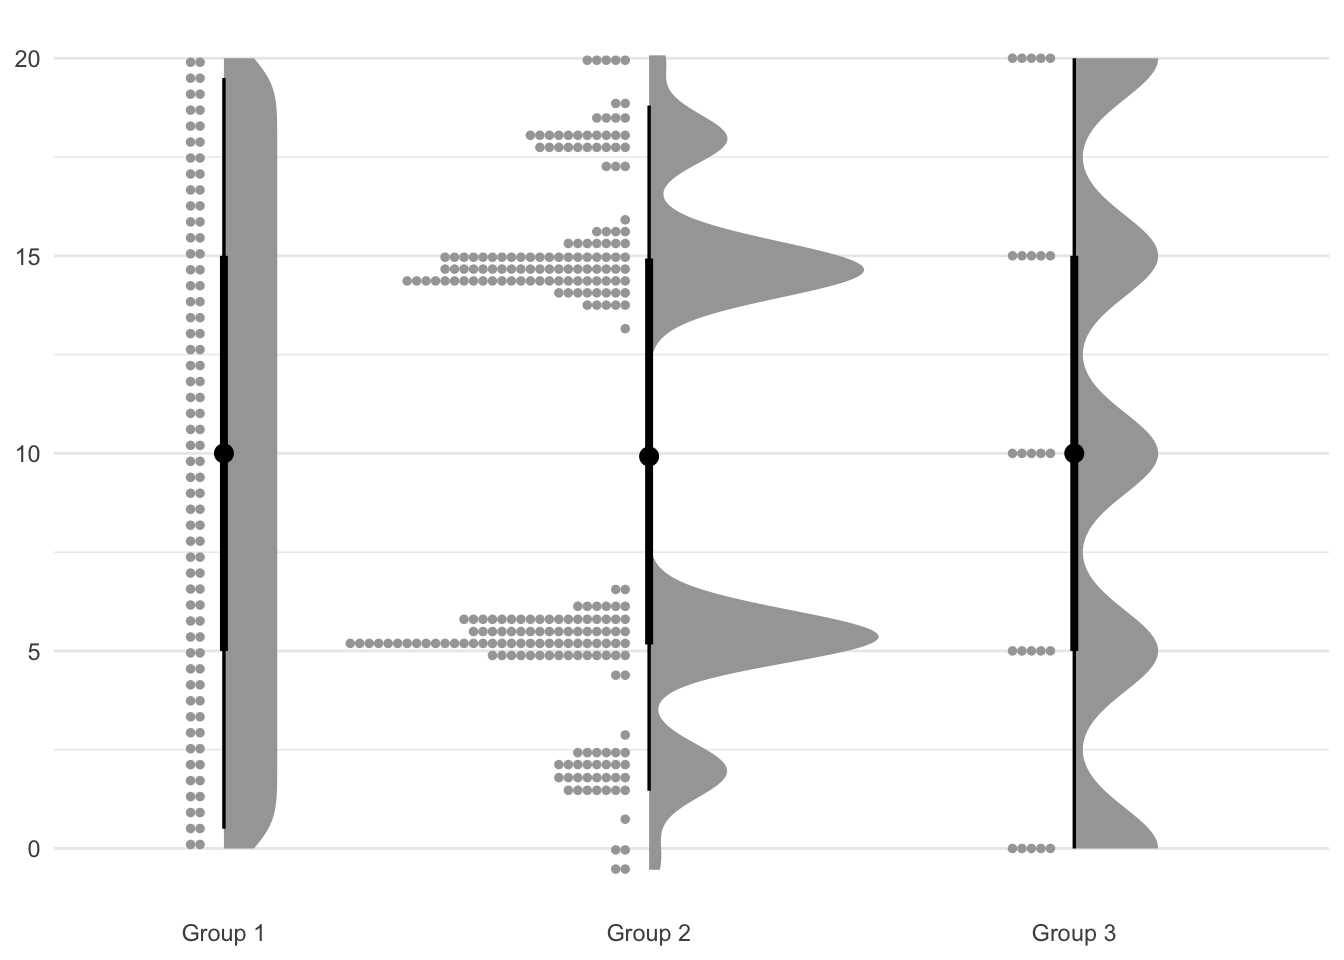
\includegraphics{./color_files/figure-pdf/unnamed-chunk-15-1.pdf}

}

\end{figure}

\hypertarget{prebuilt}{%
\subsection{Prebuilt}\label{prebuilt}}

Prebuilt color scales like ``Viridis'' are designed with perceptual
uniformity in mind, which makes them visually appealing and easy to
interpret. They provide a consistent and standardized color scheme,
eliminating the need for custom design and testing. In addition,
prebuilt color scales can help people with color blindness to better
interpret data visualizations, as they use colors with consistent visual
contrast. Using prebuilt color scales can help ensure that data
visualizations are accessible to the widest possible audience.

\begin{Shaded}
\begin{Highlighting}[]
\NormalTok{(viridis }\SpecialCharTok{|}\NormalTok{ p12) }\SpecialCharTok{+} 
\NormalTok{  patchwork}\SpecialCharTok{::}\FunctionTok{plot\_layout}\NormalTok{(}\AttributeTok{widths =} \FunctionTok{c}\NormalTok{(}\DecValTok{1}\NormalTok{,}\DecValTok{3}\NormalTok{)) }\SpecialCharTok{+} 
  \FunctionTok{plot\_annotation}\NormalTok{(}\AttributeTok{title =} \StringTok{"Virdis"}\NormalTok{,}
                  \AttributeTok{theme =} \FunctionTok{theme}\NormalTok{(}\AttributeTok{plot.title =} \FunctionTok{element\_text}\NormalTok{(}\AttributeTok{size =} \DecValTok{16}\NormalTok{)))}
\end{Highlighting}
\end{Shaded}

\begin{figure}[H]

{\centering 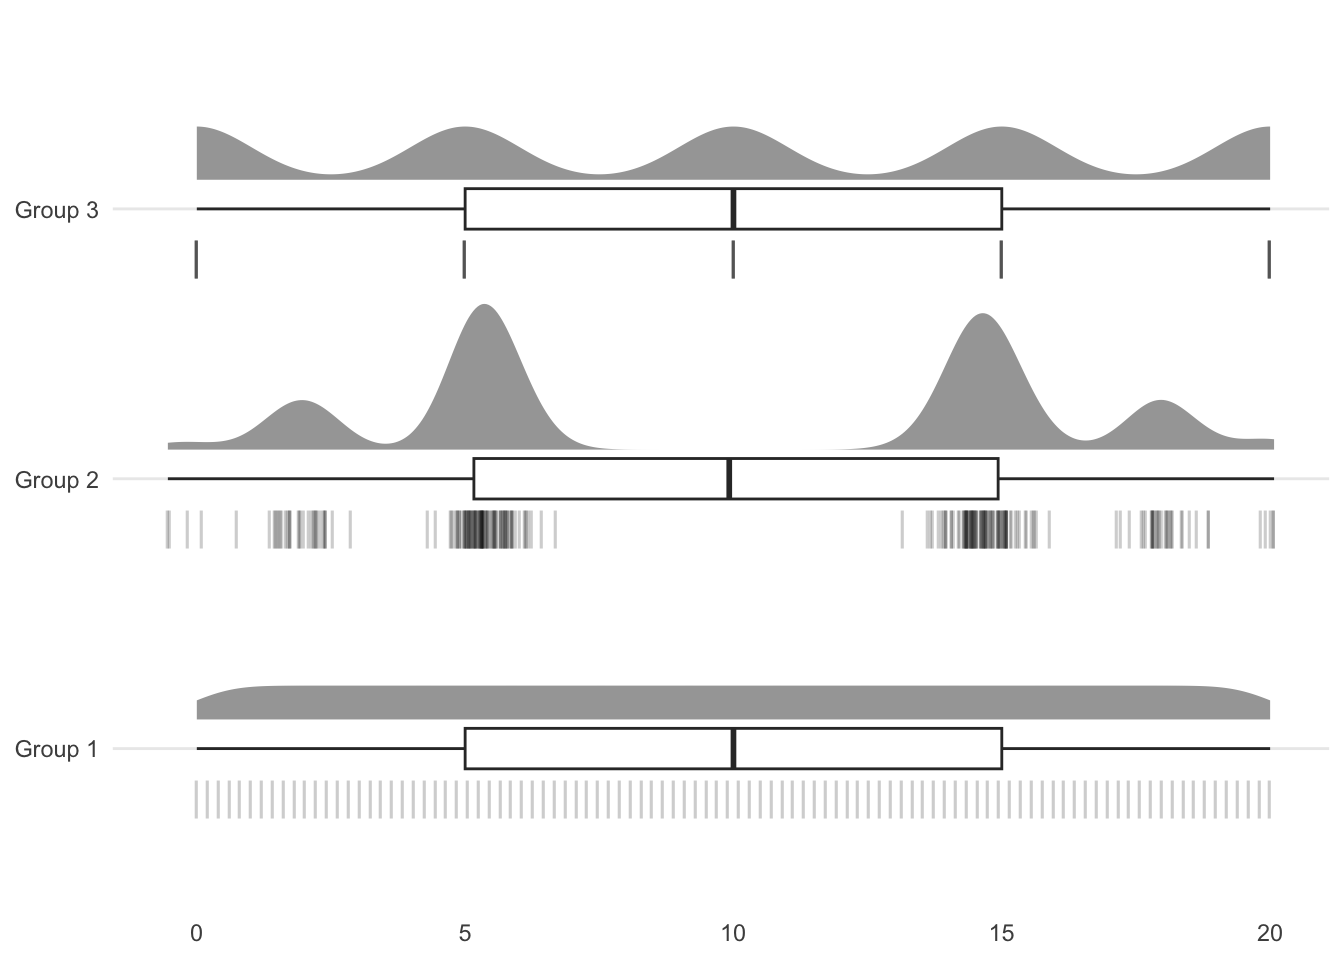
\includegraphics{./color_files/figure-pdf/unnamed-chunk-16-1.pdf}

}

\end{figure}

\hypertarget{color-systems}{%
\section{Color Systems}\label{color-systems}}

There are several popular color systems that are commonly used in
digital design and data visualization. The sRGB color system is the
standard color space used for displaying images and graphics on digital
displays. It is a device-dependent color space that is designed to
provide consistent color reproduction across a wide range of devices.
The HCV color system is based on hue, chroma, and value, and is used to
create visually distinct color palettes for use in data visualization.
The HSL color system is based on hue, saturation, and lightness, and is
often used to create color palettes for web design and user interfaces.
The LAB color system is a device-independent color space that is
designed to accurately represent colors across different devices and
environments. It is often used in professional printing and color
management applications. Each of these color systems has its own
strengths and weaknesses, and the choice of which one to use depends on
the specific needs of the project.

To see how these spaces look, check out this amazing video!

\url{https://youtu.be/HlDySNpGbyc}

\hypertarget{hsl}{%
\subsection{HSL}\label{hsl}}

The HSL color system describes colors using three parameters: hue,
saturation, and lightness. Hue is represented by a value from 0 to 360
degrees on the color wheel, and determines the basic color of the pixel.
Saturation represents the purity of the hue, or how much gray is mixed
into the color. Saturation ranges from 0\% (gray) to 100\% (pure hue).
Lightness, on the other hand, represents the amount of white or black
mixed with the color, with 0\% being black, 50\% being the original
color, and 100\% being white. HSL is often used in graphic design and
web development, as it allows for the easy selection of colors based on
hue, saturation, and lightness. However, it has some limitations, such
as not being perceptually uniform, meaning that changes in the numeric
values of the parameters may not correspond to equal changes in the
perceived color.

\hypertarget{hsv}{%
\subsection{HSV}\label{hsv}}

The HSV color system describes colors using three parameters: hue,
saturation, and value. Hue and saturation are the same as in HSL. Value
represents the brightness of the pixel, with 0\% being black and 100\%
being the brightest possible color. The HSV color system is often used
in graphics and image editing software, as it allows for easy selection
of colors. However, it is also not perceptually uniform.

\hypertarget{hcl-my-favorite}{%
\subsection{HCL (my favorite)}\label{hcl-my-favorite}}

HCL color is a perceptually uniform color space used in data
visualization and scientific applications. It consists of three values:
hue, chroma, and lightness, which represent the color, saturation, and
brightness of a color, respectively. Due to its ability to mimic human
perception of color, HCL color space is becoming increasingly popular in
design and user interface applications.

\hypertarget{lab}{%
\subsection{LAB}\label{lab}}

The LAB color system is a device-independent color space that is
designed to accurately represent colors across different devices and
environments. It consists of three parameters: L (lightness), a (the
position between red/magenta and green), and b (the position between
yellow and blue). The L parameter represents the brightness of the
color, ranging from 0 (black) to 100 (white). The a and b parameters
represent the color channels, with positive values representing colors
in the red, and yellow directions, respectively, and negative values
representing colors in green and blue direction. The LAB color space is
used in professional printing and color management applications, as it
allows for accurate color matching across different devices and
environments. Additionally, more recent LAB color spaces (ex. OKLAB) are
perceptually uniform, meaning that equal distances in LAB color space
correspond to equal steps in perceived color difference.

\hypertarget{oklab}{%
\subsection{OKLAB}\label{oklab}}

OKLAB is a color space designed to be more perceptually uniform than
other color spaces like sRGB or LAB. It uses an opponent color model,
where the color information is encoded L -- perceived lightness a -- how
green/red the color is b -- how blue/yellow the color is. This means
that the OKLAB color space can accurately represent colors while
maintaining perceptual uniformity. OKLAB was developed to address the
limitations of other color spaces. The use of OKLAB is becoming
increasingly popular in digital design and data visualization, as it can
provide more accurate and consistent color representation. You can learn
about OKLAB from the video folder.

\hypertarget{perceptual-uniformity}{%
\subsection{Perceptual Uniformity}\label{perceptual-uniformity}}

Humans are not machines, we wee see things with our eyes and process
them with our brain. What might appear like a similar color to a machine
for humans will not. As an example, below are two color wheels one is
RGB (perceptually non-uniform) and the other is HCL (uniform). When the
color spectra are viewed in Gray scale the uneven nature of RGB becomes
apparent. A technical definition is that a perceptual uniform color
space ensures that the difference between two colors (as perceived by
the human eye) is proportional to the Euclidian distance within the
given color space.

\begin{figure}

{\centering 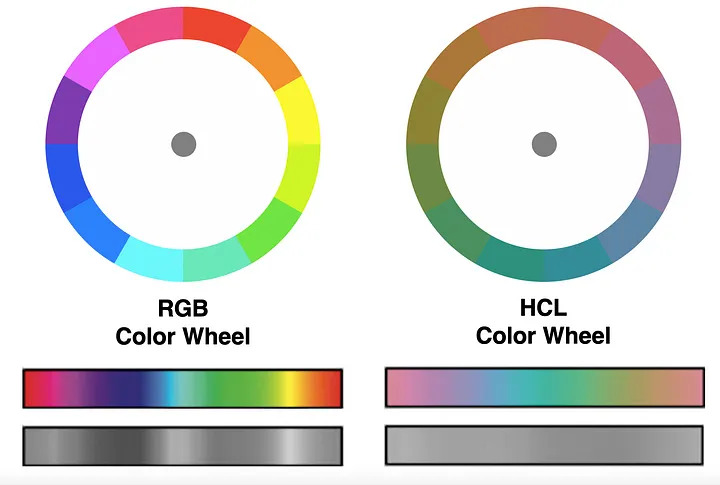
\includegraphics{./images/uniform_perception.jpg}

}

\caption{uniform perception}

\end{figure}

\hypertarget{warning-colormaps-might-increase-risk-of-death}{%
\subsubsection{Warning Colormaps might Increase Risk of
Death!}\label{warning-colormaps-might-increase-risk-of-death}}

In 1990s data visualization specialists adopted Rainbow Color Map with
the most famous variation being Jet default palette. Many researchers
expressed concerns as the non-uniform nature of the palette introduced
transitions that could be perceived incorrectly.

Rogowitz and Treinish raised concerns about the Rainbow Color Map in
1998 ``Data Visualization: The End of the Rainbow''(Rogowitz and
Treinish
1998)\marginpar{\begin{footnotesize}\leavevmode\vadjust pre{\protect\hypertarget{ref-rogowitzDataVisualizationEnd1998}{}}%
Rogowitz, B. E., and L. A. Treinish. 1998. {``Data Visualization: The
End of the Rainbow.''} \emph{IEEE Spectrum} 35 (12): 52--59.
\url{https://doi.org/10.1109/6.736450}.\vspace{2mm}\par\end{footnotesize}},
and Borland and Taylor highlighted additional concerns in a 2007 paper
``Rainbow Color Map (Still) Considered Harmful'' (Borland and Taylor Ii
2007)\marginpar{\begin{footnotesize}\leavevmode\vadjust pre{\protect\hypertarget{ref-borlandRainbowColorMap2007}{}}%
Borland, David, and Russell M. Taylor Ii. 2007. {``Rainbow Color Map
(Still) Considered Harmful.''} \emph{IEEE Computer Graphics and
Applications} 27 (2): 14--17.
\url{https://doi.org/10.1109/MCG.2007.323435}.\vspace{2mm}\par\end{footnotesize}}.
In 2011, Borkin and her team conducted user studies on the application
of various color maps, including the Rainbow Color map, to medical
visualization problems. Their findings in ``Evaluation of Artery
Visualizations of Heart Disease Diagnosis'' (Borkin et al.
2011)\marginpar{\begin{footnotesize}\leavevmode\vadjust pre{\protect\hypertarget{ref-borkinEvaluationArteryVisualizations2011}{}}%
Borkin, M., K. Gajos, A. Peters, D. Mitsouras, S. Melchionna, F.
Rybicki, C. Feldman, and H. Pfister. 2011. {``Evaluation of Artery
Visualizations for Heart Disease Diagnosis.''} \emph{IEEE Transactions
on Visualization and Computer Graphics} 17 (12): 2479--88.
\url{https://doi.org/10.1109/TVCG.2011.192}.\vspace{2mm}\par\end{footnotesize}}
showed that a perceptually uniform color map resulted in fewer
diagnostic errors than the Rainbow Color map. So, diagnostic errors
could be reduced by simply switching to a proper color palette. The
problem of misuse of color still persists as outlined by Crameri,
Shephard and Heron in ``The misuse of colour in science communication''
(2020) (Crameri, Shephard, and Heron
2020)\marginpar{\begin{footnotesize}\leavevmode\vadjust pre{\protect\hypertarget{ref-crameriMisuseColourScience2020}{}}%
Crameri, Fabio, Grace E. Shephard, and Philip J. Heron. 2020. {``The
Misuse of Colour in Science Communication.''} \emph{Nature
Communications} 11 (1): 5444.
\url{https://doi.org/10.1038/s41467-020-19160-7}.\vspace{2mm}\par\end{footnotesize}}
-- a paper that I believe must be read by any scientist.

\begin{figure}

{\centering 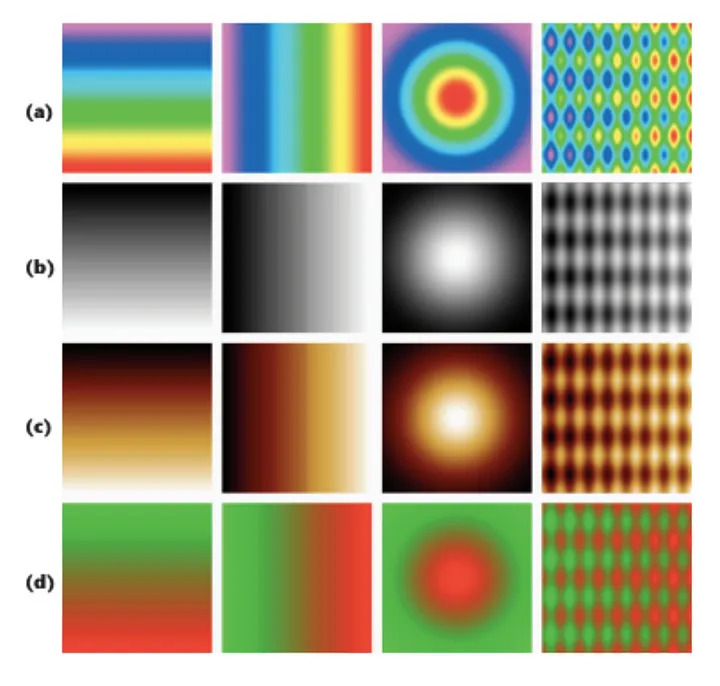
\includegraphics{./images/jet_comparison.jpg}

}

\caption{Image from the ``Rainbow Color Map (Still Considered Harmful)}

\end{figure}

All of these issues are amplified once we consider that roughly 8\% of
all men and 0.5\% of all women are colorblind. There are three main
forms of red(protan), gren(deutan), and blue (tritan) disorders,
corresponding to color sensitive cones in our eyes. To check whether
your visualization is colorblind friendly use
\href{https://www.color-blindness.com/coblis-color-blindness-simulator/}{Coblis}
({``Coblis {\textemdash} Color Blindness Simulator {\textendash}
Colblindor,''}
n.d.)\marginpar{\begin{footnotesize}\leavevmode\vadjust pre{\protect\hypertarget{ref-CoblisColorBlindness}{}}%
{``Coblis {\textemdash} Color Blindness Simulator {\textendash}
Colblindor.''} n.d.
\url{https://www.color-blindness.com/coblis-color-blindness-simulator/}.\vspace{2mm}\par\end{footnotesize}}.

To improve the readability of your colors vary their value and hue, but
try not to include both red and green into your graphics as red-green
colorblindness is the most common.

\begin{figure}

{\centering 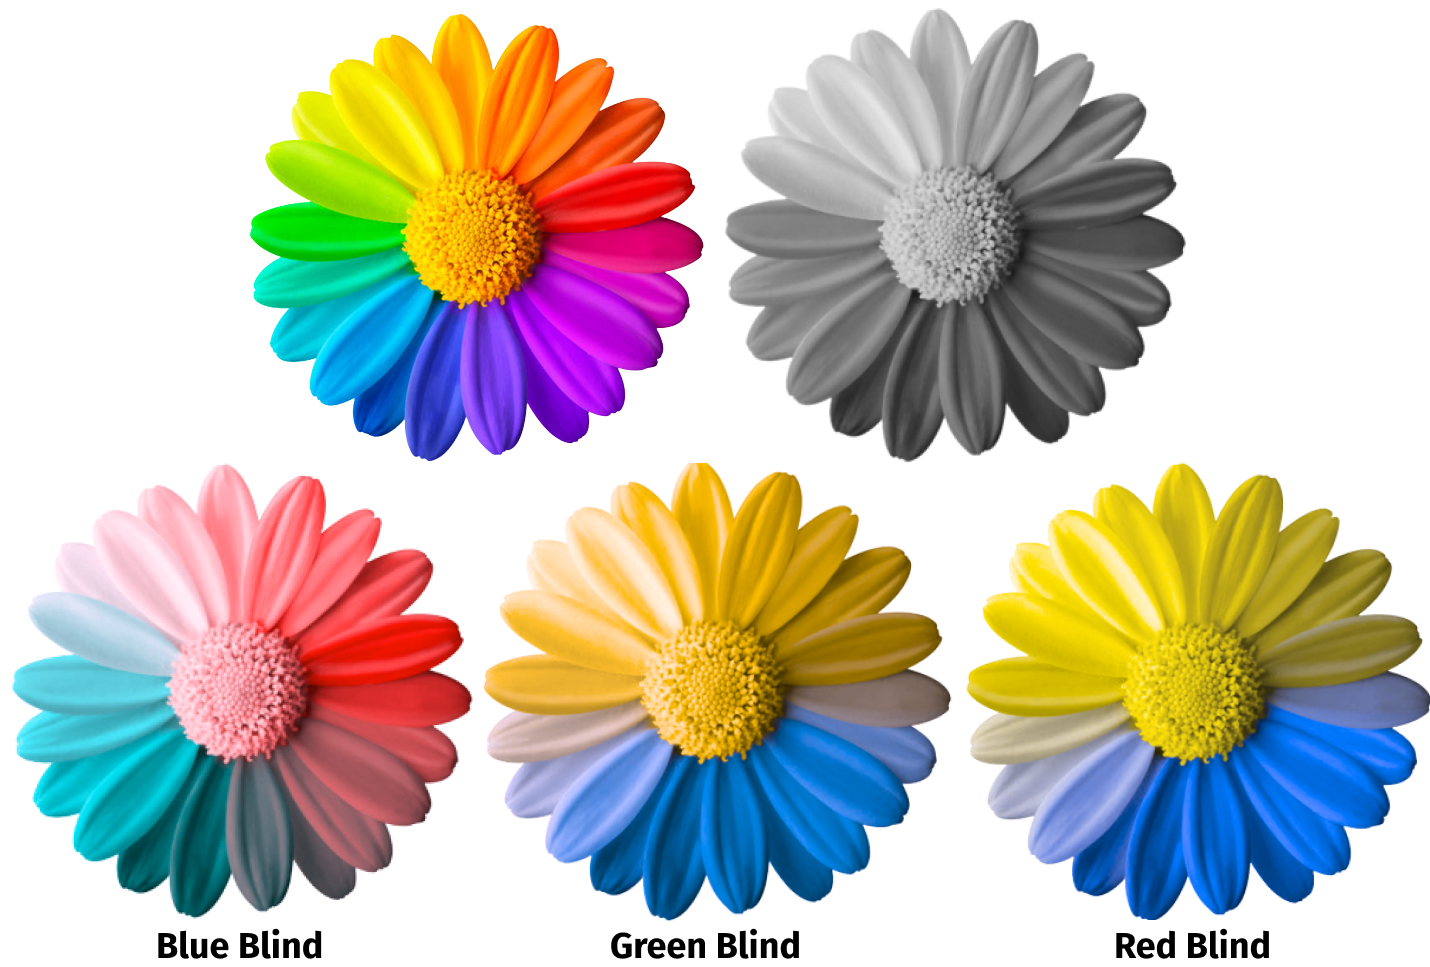
\includegraphics[width=6.92708in,height=\textheight]{./images/Color_Blindness.jpg}

}

\caption{Color Blind Rainbow Flower}

\end{figure}

\hypertarget{so-what-should-you-use}{%
\subsubsection{So what should you use?}\label{so-what-should-you-use}}

A simple and correct answer would be to use a scientific color map that
you find pretty and use it as your default. If you need some help use
this graph from ``The misuse of colour in science communication''.

\begin{figure}

{\centering 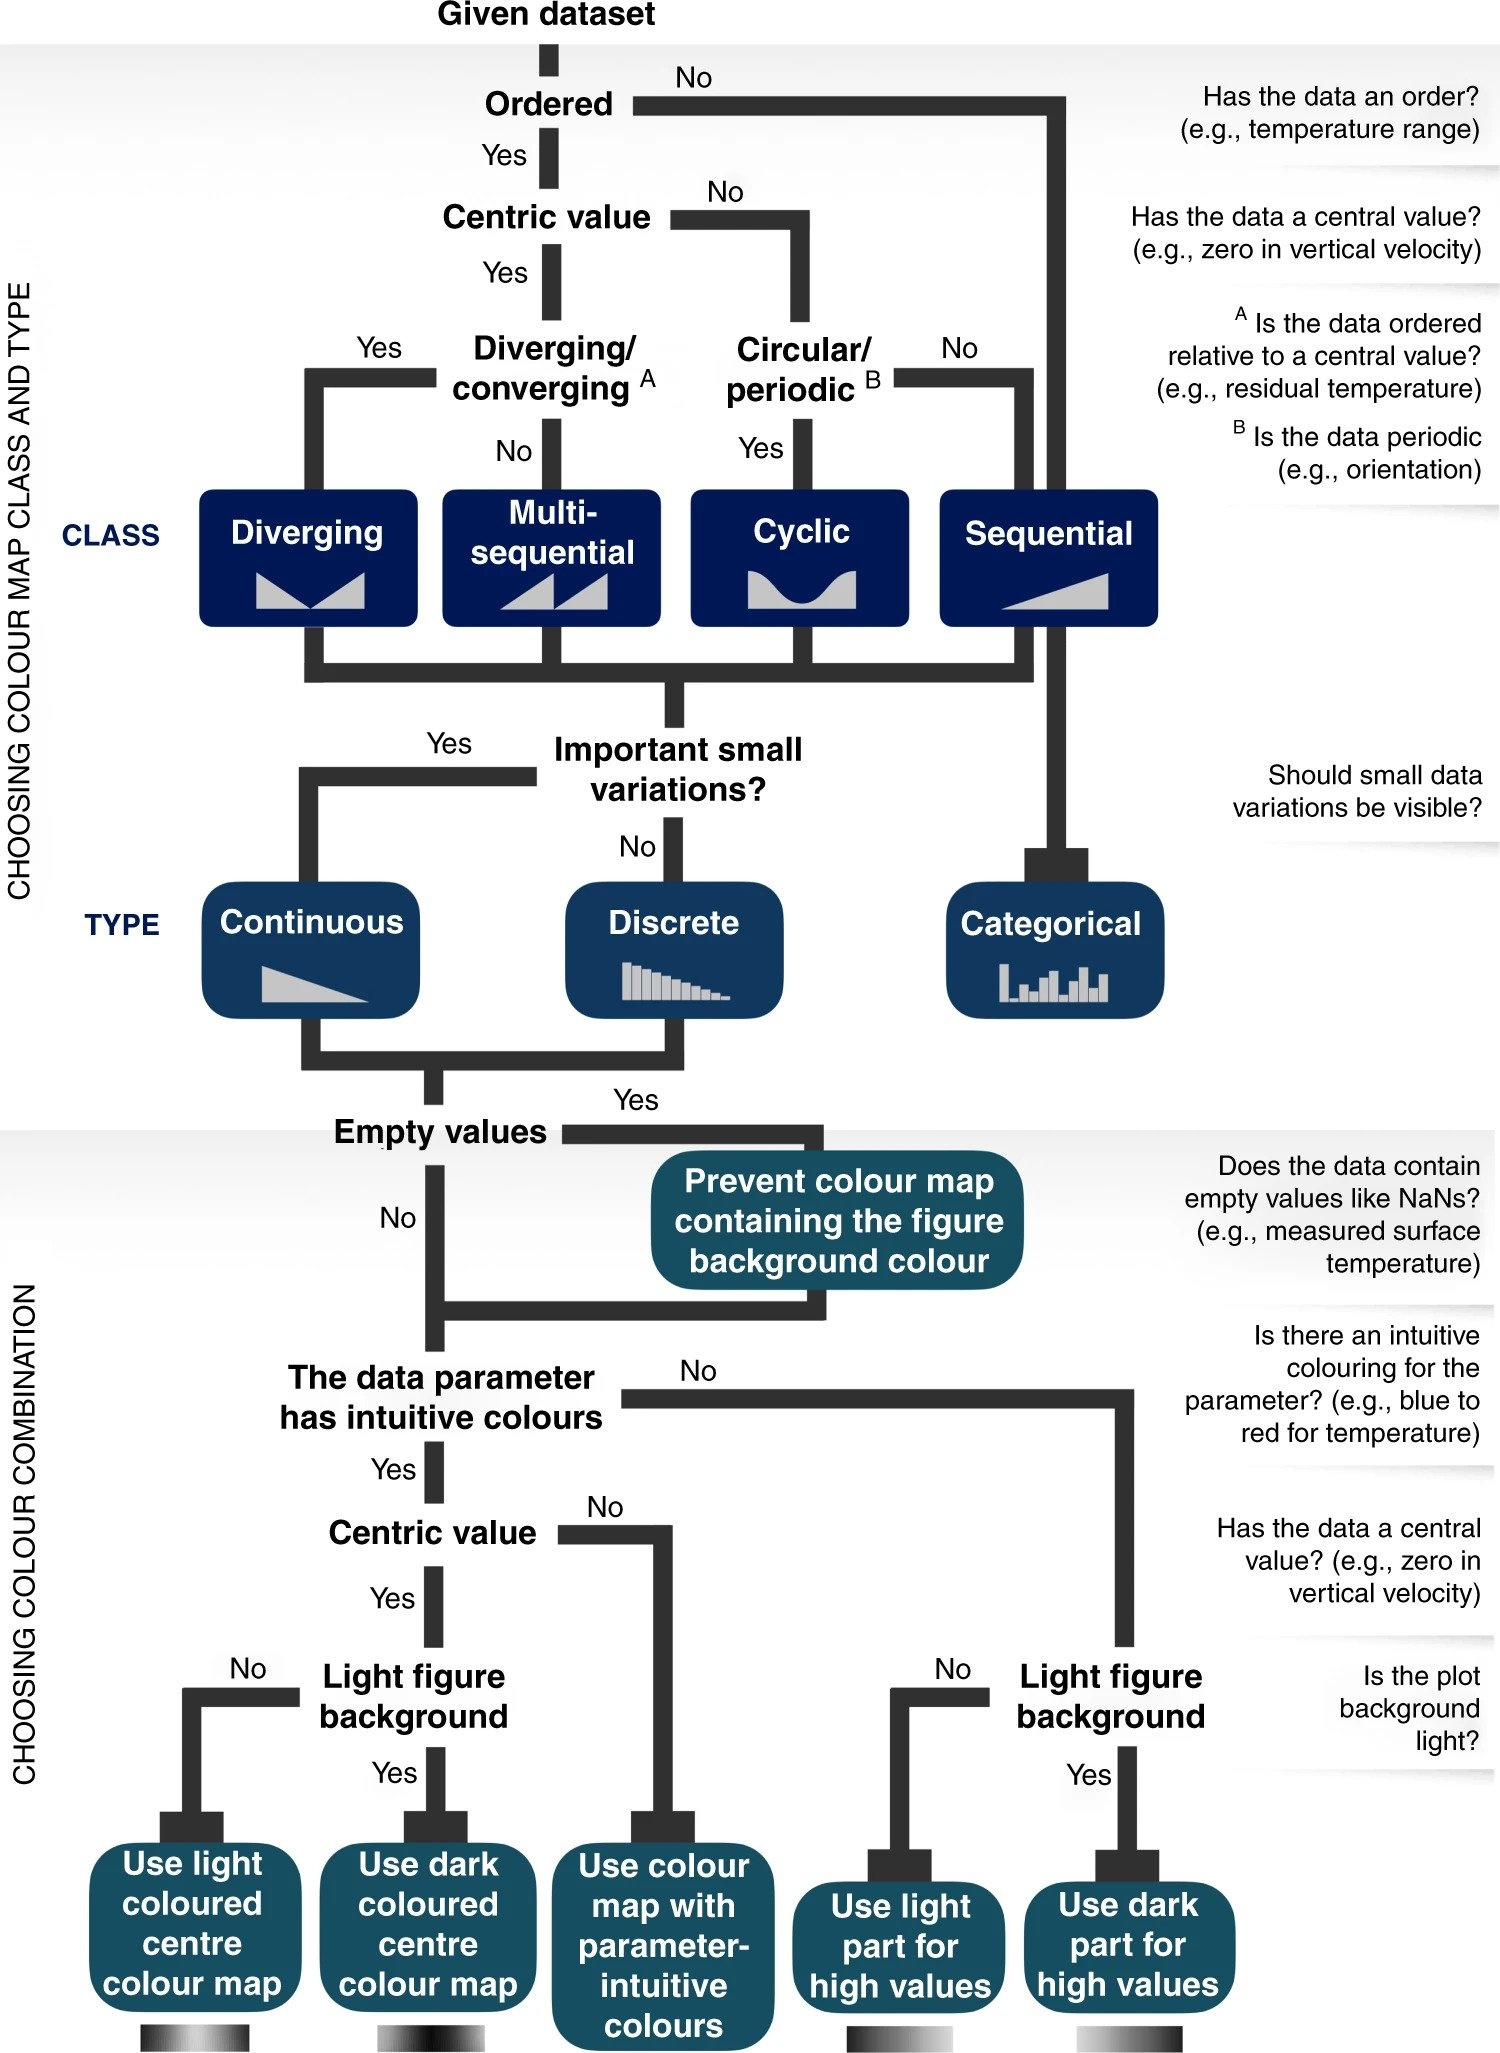
\includegraphics[width=3.80208in,height=\textheight]{./images/choosing_color_map.jpg}

}

\caption{choosing color map}

\end{figure}

If you want to pick colors yourself use HSL, because it is the most
intuitive one and the easiest to make color palettes in. I would also
recommend tinkering with OKHSL, which is a child of OKLAB and HSL
producing a perceptually uniform HSL space. Try out both of them and see
the difference
\href{https://bottosson.github.io/misc/colorpicker/}{here}\sidenote{\footnotesize https://bottosson.github.io/misc/colorpicker/}.

\hypertarget{where-do-i-find-color-waves}{%
\subsection{Where do I find color
waves?}\label{where-do-i-find-color-waves}}

\href{https://color.adobe.com/create/color-wheel}{Adobe Color} - Adobe
Color let's you create color palettes using different color harmony
rules and color modes. You can also pick colors from your image, make
gradients from images, and test for accessibility.

\href{https://paletton.com/}{Paletton} - Amazing tool for creating color
palettes

\href{http://colorbrewer2.org/}{Color Brewer} - Color Brewer is a
web-based tool that provides color schemes perceptual uniform for maps
and data visualizations.

\href{https://lokeshdhakar.com/projects/color-thief/}{Color Thief} -
Color Thief let's you extract colors from your image to create
nature-inspired palettes.

\href{https://projects.susielu.com/viz-palette}{Viz Palette} - Viz
Palette can be used to check your color palettes before creating
visualizations. It allows you to view color sets in example plots,
simulate color deficiencies, and modify the colors of your palette.

\href{https://www.fabiocrameri.ch/colourmaps/}{Scientific colour maps} -
A collection of uniform and readable color maps for scientific use.

\hypertarget{whats-next}{%
\section{What's next?}\label{whats-next}}

\hypertarget{a-graph-for-the-job}{%
\chapter{A Graph for The Job}\label{a-graph-for-the-job}}

When working on graphs don't think ``what chart should I use?'', but
``what am I trying to show?'' In this section we will look at different
types of chart, what they show and when to use them. We will not cover
all the graphs, but you will definitely expand your kit!

Graphs for category comparison are a type of data visualization that are
used to compare and contrast different categories or groups. The most
common of them is bar chart! The one below shows the top 5 countries by
GDP per Capita in 1997. You can easily see that Norway is first and
Switzerland is 5th!

\begin{Shaded}
\begin{Highlighting}[]
\NormalTok{gapminder }\SpecialCharTok{\%\textgreater{}\%} \FunctionTok{filter}\NormalTok{(year }\SpecialCharTok{==} \DecValTok{1997}\NormalTok{) }\SpecialCharTok{\%\textgreater{}\%} \FunctionTok{slice\_max}\NormalTok{(gdpPercap, }\AttributeTok{n =} \DecValTok{5}\NormalTok{) }\SpecialCharTok{\%\textgreater{}\%} \FunctionTok{ggplot}\NormalTok{(}\FunctionTok{aes}\NormalTok{(}\AttributeTok{x =} \FunctionTok{fct\_reorder}\NormalTok{(country,gdpPercap,}\AttributeTok{.desc =}\NormalTok{ T), }\AttributeTok{y =}\NormalTok{ gdpPercap)) }\SpecialCharTok{+} \FunctionTok{geom\_col}\NormalTok{(}\AttributeTok{fill =} \StringTok{"steelblue"}\NormalTok{) }\SpecialCharTok{+} \FunctionTok{theme\_minimal}\NormalTok{(}\AttributeTok{base\_size =} \DecValTok{18}\NormalTok{) }\SpecialCharTok{+} \FunctionTok{labs}\NormalTok{(}\AttributeTok{x =} \ConstantTok{NULL}\NormalTok{, }\AttributeTok{y =} \ConstantTok{NULL}\NormalTok{, }\AttributeTok{title =} \StringTok{"Top 5 countries by GDP per Capita in 1997"}\NormalTok{) }\SpecialCharTok{+} 
\FunctionTok{geom\_text}\NormalTok{(}\FunctionTok{aes}\NormalTok{(}\AttributeTok{label =} \FunctionTok{round}\NormalTok{(gdpPercap,}\DecValTok{0}\NormalTok{)), }\AttributeTok{vjust =} \DecValTok{10}\NormalTok{, }\AttributeTok{color =} \StringTok{"white"}\NormalTok{, }\AttributeTok{size =} \DecValTok{5}\NormalTok{) }\SpecialCharTok{+} 
\FunctionTok{theme}\NormalTok{(}\AttributeTok{panel.grid =} \FunctionTok{element\_blank}\NormalTok{(), }\AttributeTok{axis.text.y =} \FunctionTok{element\_blank}\NormalTok{())}
\end{Highlighting}
\end{Shaded}

\begin{figure}[H]

{\centering 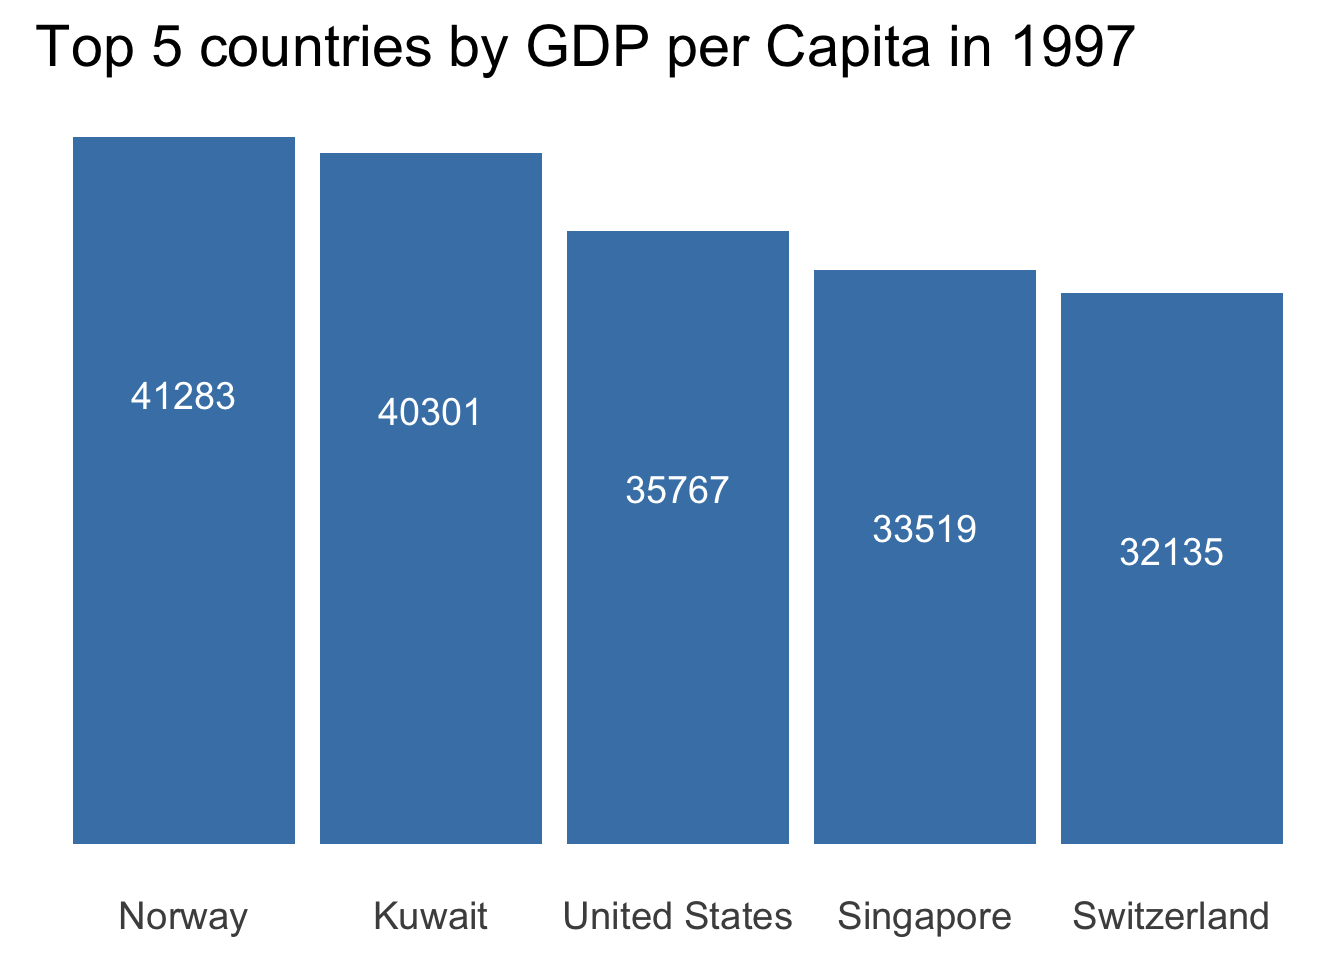
\includegraphics{./which_graph_files/figure-pdf/unnamed-chunk-2-1.pdf}

}

\end{figure}

Vertical bar charts are great to provide a quick comparison for a small
number of categories (less than 7). But if need to show ranking of more
things, flip the axis of the bar chart! Additional bonus, horizontal bar
charts are great if you have long names to display. Below are the
results of the 2021 London election. British YouTuber Niko Omilana
finished 5th \emph{for the memes}! Max Fosh, another YouTuber, also
passed the cut off!

\begin{Shaded}
\begin{Highlighting}[]
\NormalTok{barh\_data }\OtherTok{\textless{}{-}} \FunctionTok{tibble}\NormalTok{(}\AttributeTok{Candidate =} \FunctionTok{c}\NormalTok{(}\StringTok{"Sadiq Khan"}\NormalTok{, }\StringTok{"Shaun Bailey"}\NormalTok{, }\StringTok{"Siân Berry"}\NormalTok{, }
\StringTok{"Luisa Porritt"}\NormalTok{, }\StringTok{"Niko Omilana"}\NormalTok{, }\StringTok{"Laurence Fox"}\NormalTok{, }\StringTok{"Brian Rose"}\NormalTok{, }
\StringTok{"Richard Hewison"}\NormalTok{, }\StringTok{"Count Binface"}\NormalTok{, }\StringTok{"Mandu Reid"}\NormalTok{, }\StringTok{"Piers Corbyn"}\NormalTok{, }
\StringTok{"Vanessa Hudson"}\NormalTok{, }\StringTok{"Peter Gammons"}\NormalTok{, }\StringTok{"Farah London"}\NormalTok{, }\StringTok{"David Kurten"}\NormalTok{, }
\StringTok{"Nims Obunge"}\NormalTok{, }\StringTok{"Steve Kelleher"}\NormalTok{, }\StringTok{"Kam Balayev"}\NormalTok{, }\StringTok{"Max Fosh"}\NormalTok{, }\StringTok{"Valerie Brown"}
\NormalTok{), }
\AttributeTok{Percentage =} \FunctionTok{c}\NormalTok{(}\FloatTok{40.0}\NormalTok{, }\FloatTok{35.3}\NormalTok{, }\FloatTok{7.8}\NormalTok{, }\FloatTok{4.4}\NormalTok{, }\FloatTok{2.0}\NormalTok{, }\FloatTok{1.9}\NormalTok{, }
\FloatTok{1.2}\NormalTok{, }\FloatTok{1.1}\NormalTok{, }\FloatTok{1.0}\NormalTok{, }\FloatTok{0.8}\NormalTok{, }\FloatTok{0.8}\NormalTok{, }\FloatTok{0.7}\NormalTok{, }\FloatTok{0.6}\NormalTok{, }\FloatTok{0.5}\NormalTok{, }\FloatTok{0.4}\NormalTok{, }
\FloatTok{0.4}\NormalTok{, }\FloatTok{0.3}\NormalTok{, }\FloatTok{0.3}\NormalTok{, }\FloatTok{0.2}\NormalTok{, }\FloatTok{0.2}\NormalTok{)) }\SpecialCharTok{\%\textgreater{}\%} \FunctionTok{mutate}\NormalTok{(}\AttributeTok{is.youtuber =} \FunctionTok{case\_when}\NormalTok{(}
\NormalTok{  Candidate }\SpecialCharTok{==} \StringTok{"Niko Omilana"} \SpecialCharTok{\textasciitilde{}} \DecValTok{1}\NormalTok{,}
\NormalTok{  Candidate }\SpecialCharTok{==} \StringTok{"Max Fosh"} \SpecialCharTok{\textasciitilde{}} \DecValTok{2}\NormalTok{,}
\NormalTok{  T }\SpecialCharTok{\textasciitilde{}} \DecValTok{0}\NormalTok{))}
\end{Highlighting}
\end{Shaded}

\begin{Shaded}
\begin{Highlighting}[]
\NormalTok{barh\_data }\SpecialCharTok{\%\textgreater{}\%}
\FunctionTok{ggplot}\NormalTok{(}\FunctionTok{aes}\NormalTok{(}\AttributeTok{x =} \FunctionTok{fct\_reorder}\NormalTok{(Candidate, Percentage), }\AttributeTok{y =}\NormalTok{ Percentage, }\AttributeTok{fill =} \FunctionTok{as.factor}\NormalTok{(is.youtuber))) }\SpecialCharTok{+}
\FunctionTok{geom\_col}\NormalTok{() }\SpecialCharTok{+} 
\FunctionTok{theme\_minimal}\NormalTok{(}\AttributeTok{base\_size =} \DecValTok{16}\NormalTok{) }\SpecialCharTok{+} 
\FunctionTok{coord\_flip}\NormalTok{() }\SpecialCharTok{+} 
\FunctionTok{labs}\NormalTok{(}\AttributeTok{x =} \ConstantTok{NULL}\NormalTok{, }\AttributeTok{y =} \ConstantTok{NULL}\NormalTok{, }\AttributeTok{title =} \StringTok{"London Mayor Elections (2021) by \% of Votes"}\NormalTok{) }\SpecialCharTok{+} 
\FunctionTok{theme}\NormalTok{(}\AttributeTok{panel.grid =} \FunctionTok{element\_blank}\NormalTok{(), }\AttributeTok{legend.position =} \StringTok{"none"}\NormalTok{, }\AttributeTok{plot.caption.position =} \StringTok{"plot"}\NormalTok{) }\SpecialCharTok{+} 
\FunctionTok{scale\_y\_discrete}\NormalTok{(}\AttributeTok{expand =} \FunctionTok{c}\NormalTok{(}\DecValTok{0}\NormalTok{,}\DecValTok{0}\NormalTok{,}\DecValTok{0}\NormalTok{,}\DecValTok{3}\NormalTok{)) }\SpecialCharTok{+} 
\FunctionTok{geom\_text}\NormalTok{(}\FunctionTok{aes}\NormalTok{(}\AttributeTok{label =}\NormalTok{ Percentage), }\AttributeTok{nudge\_y =} \FloatTok{0.3}\NormalTok{, }\AttributeTok{hjust =} \StringTok{"left"}\NormalTok{)  }\SpecialCharTok{+} 
\FunctionTok{scale\_fill\_manual}\NormalTok{(}\AttributeTok{values =} \FunctionTok{c}\NormalTok{(}\StringTok{"\#c0bfff"}\NormalTok{,}\StringTok{"\#f3e408"}\NormalTok{,}\StringTok{"\#D96161"}\NormalTok{)) }
\end{Highlighting}
\end{Shaded}

\begin{figure}[H]

{\centering \includegraphics{./which_graph_files/figure-pdf/unnamed-chunk-3-1.pdf}

}

\end{figure}

\hypertarget{distribution}{%
\section{Distribution}\label{distribution}}

\hypertarget{histogram}{%
\subsection{Histogram}\label{histogram}}

What if you want to show the distribution of the data? We can use a
variation of a bar chart -- histogram! Histograms show the distribution
of continuous data by grouping it into bins and displaying the frequency
or proportion of observations that fall into each bin. They are great if
you want to show the shape of the distribution, but they are very
sensitive to the bins you choose. Notice how the shape of the
distribution changes for each number of bins. It is important to strike
a balance between too few and too many. 6 bins makes our distribution
look pretty normal while 30 bins make it all over the place. 15 bins
seems about right it preserves the bimodal feature of the distribution,
while keeping the picture legible.

\begin{Shaded}
\begin{Highlighting}[]
\NormalTok{base }\OtherTok{\textless{}{-}}\NormalTok{ iris }\SpecialCharTok{\%\textgreater{}\%} \FunctionTok{ggplot}\NormalTok{(}\FunctionTok{aes}\NormalTok{(}\AttributeTok{x =}\NormalTok{ Sepal.Length))  }\SpecialCharTok{+} \FunctionTok{theme\_minimal}\NormalTok{() }\SpecialCharTok{+} \FunctionTok{theme}\NormalTok{(}\AttributeTok{panel.grid =} \FunctionTok{element\_blank}\NormalTok{(), }\AttributeTok{axis.text.y =} \FunctionTok{element\_blank}\NormalTok{()) }\SpecialCharTok{+} 
  \FunctionTok{coord\_cartesian}\NormalTok{(}\AttributeTok{expand =} \ConstantTok{FALSE}\NormalTok{, }\AttributeTok{clip =} \StringTok{"off"}\NormalTok{) }\SpecialCharTok{+} \FunctionTok{labs}\NormalTok{(}\AttributeTok{y =} \ConstantTok{NULL}\NormalTok{, }\AttributeTok{x =} \ConstantTok{NULL}\NormalTok{)}
\NormalTok{hist\_1 }\OtherTok{\textless{}{-}}\NormalTok{ base }\SpecialCharTok{+} \FunctionTok{geom\_histogram}\NormalTok{(}\AttributeTok{fill =} \StringTok{"steelblue"}\NormalTok{, }\AttributeTok{color =} \StringTok{"white"}\NormalTok{, }\AttributeTok{bins =} \DecValTok{6}\NormalTok{) }\SpecialCharTok{+} \FunctionTok{labs}\NormalTok{(}\AttributeTok{subtitle =} \StringTok{"6 bins"}\NormalTok{)}
\NormalTok{hist\_2 }\OtherTok{\textless{}{-}}\NormalTok{ base }\SpecialCharTok{+} \FunctionTok{geom\_histogram}\NormalTok{(}\AttributeTok{fill =} \StringTok{"steelblue"}\NormalTok{, }\AttributeTok{color =} \StringTok{"white"}\NormalTok{, }\AttributeTok{bins =} \DecValTok{15}\NormalTok{) }\SpecialCharTok{+} \FunctionTok{labs}\NormalTok{(}\AttributeTok{subtitle =} \StringTok{"15 bins"}\NormalTok{)}
\NormalTok{hist\_3 }\OtherTok{\textless{}{-}}\NormalTok{ base }\SpecialCharTok{+} \FunctionTok{geom\_histogram}\NormalTok{(}\AttributeTok{fill =} \StringTok{"steelblue"}\NormalTok{, }\AttributeTok{color =} \StringTok{"white"}\NormalTok{, }\AttributeTok{bins =} \DecValTok{30}\NormalTok{) }\SpecialCharTok{+} \FunctionTok{labs}\NormalTok{(}\AttributeTok{subtitle =} \StringTok{"30 bins"}\NormalTok{)}

\NormalTok{(hist\_1 }\SpecialCharTok{+}\NormalTok{ hist\_2 }\SpecialCharTok{+}\NormalTok{ hist\_3) }\SpecialCharTok{+} \FunctionTok{plot\_annotation}\NormalTok{(}\AttributeTok{title =} \StringTok{"iris Sepal Length Distribution Histograms with Varying Bins"}\NormalTok{)}
\end{Highlighting}
\end{Shaded}

\begin{figure}[H]

{\centering \includegraphics{./which_graph_files/figure-pdf/unnamed-chunk-4-1.pdf}

}

\end{figure}

\hypertarget{density-plot}{%
\subsection{Density Plot}\label{density-plot}}

Unlike histograms, density plots use a continuous line to represent the
data instead of bars. This smooth curve provides a more detailed and
nuanced representation of the distribution of the data, allowing for
easier detection of patterns and trends. The density plot constructs
this line by placing many small normal distributions at each point in
the data, which are then used to weigh all points within their
respective range and draw a curve connecting them. The width of these
curves is controlled by the bandwidth of the density plot, which
determines how wide the curves span. A larger bandwidth will consider
more points, resulting in a smoother curve, while a smaller bandwidth
will lead to a jagged line.

\begin{Shaded}
\begin{Highlighting}[]
\NormalTok{base }\OtherTok{\textless{}{-}}\NormalTok{ iris }\SpecialCharTok{\%\textgreater{}\%} \FunctionTok{ggplot}\NormalTok{(}\FunctionTok{aes}\NormalTok{(}\AttributeTok{x =}\NormalTok{ Sepal.Length))  }\SpecialCharTok{+} \FunctionTok{theme\_minimal}\NormalTok{() }\SpecialCharTok{+} \FunctionTok{theme}\NormalTok{(}\AttributeTok{panel.grid =} \FunctionTok{element\_blank}\NormalTok{(), }\AttributeTok{axis.text.y =} \FunctionTok{element\_blank}\NormalTok{()) }\SpecialCharTok{+} 
  \FunctionTok{coord\_cartesian}\NormalTok{(}\AttributeTok{expand =} \ConstantTok{FALSE}\NormalTok{, }\AttributeTok{clip =} \StringTok{"off"}\NormalTok{) }\SpecialCharTok{+} \FunctionTok{labs}\NormalTok{(}\AttributeTok{y =} \ConstantTok{NULL}\NormalTok{, }\AttributeTok{x =} \ConstantTok{NULL}\NormalTok{)}
\NormalTok{dens\_1 }\OtherTok{\textless{}{-}}\NormalTok{ base }\SpecialCharTok{+} \FunctionTok{geom\_density}\NormalTok{(}\AttributeTok{color =} \StringTok{"steelblue"}\NormalTok{, }\AttributeTok{linewidth =} \DecValTok{2}\NormalTok{, }\AttributeTok{bw =} \FloatTok{0.3}\NormalTok{) }\SpecialCharTok{+} \FunctionTok{labs}\NormalTok{(}\AttributeTok{subtitle =} \StringTok{"Band Width 0.3"}\NormalTok{)}
\NormalTok{dens\_2 }\OtherTok{\textless{}{-}}\NormalTok{ base }\SpecialCharTok{+} \FunctionTok{geom\_density}\NormalTok{(}\AttributeTok{color =} \StringTok{"steelblue"}\NormalTok{, }\AttributeTok{linewidth =} \DecValTok{2}\NormalTok{, }\AttributeTok{bw =} \FloatTok{0.1}\NormalTok{) }\SpecialCharTok{+} \FunctionTok{labs}\NormalTok{(}\AttributeTok{subtitle =} \StringTok{"Band Width 0.1"}\NormalTok{)}
\NormalTok{dens\_3 }\OtherTok{\textless{}{-}}\NormalTok{ base }\SpecialCharTok{+} \FunctionTok{geom\_density}\NormalTok{(}\AttributeTok{color =} \StringTok{"steelblue"}\NormalTok{, }\AttributeTok{linewidth =} \DecValTok{1}\NormalTok{, }\AttributeTok{bw =} \FloatTok{0.03}\NormalTok{) }\SpecialCharTok{+} \FunctionTok{labs}\NormalTok{(}\AttributeTok{subtitle =} \StringTok{"Band Width 0.03"}\NormalTok{)}

\NormalTok{(dens\_1 }\SpecialCharTok{+}\NormalTok{ dens\_2 }\SpecialCharTok{+}\NormalTok{ dens\_3) }\SpecialCharTok{+} \FunctionTok{plot\_annotation}\NormalTok{(}\AttributeTok{title =} \StringTok{"iris Sepal Length Distribution Density Plots with Varying Band Widths"}\NormalTok{)}
\end{Highlighting}
\end{Shaded}

\begin{figure}[H]

{\centering \includegraphics{./which_graph_files/figure-pdf/unnamed-chunk-5-1.pdf}

}

\end{figure}

\hypertarget{frequency-polygon}{%
\subsection{Frequency Polygon}\label{frequency-polygon}}

It is similar to a histogram, but instead of bars, it uses a continuous
line to connect the points representing the frequencies. Frequency
polygons are particularly useful when comparing two or more data sets on
the same plot. Just like histogram it relies on the selection of bins.

\begin{Shaded}
\begin{Highlighting}[]
\NormalTok{freq\_1 }\OtherTok{\textless{}{-}}\NormalTok{ base }\SpecialCharTok{+} \FunctionTok{geom\_histogram}\NormalTok{(}\AttributeTok{fill =} \StringTok{"grey"}\NormalTok{, }\AttributeTok{color =} \StringTok{"white"}\NormalTok{, }\AttributeTok{bins =} \DecValTok{15}\NormalTok{, }\AttributeTok{alpha =} \FloatTok{0.5}\NormalTok{) }\SpecialCharTok{+} \FunctionTok{geom\_freqpoly}\NormalTok{(}\AttributeTok{color =} \StringTok{"steelblue"}\NormalTok{, }\AttributeTok{bins =} \DecValTok{15}\NormalTok{, }\AttributeTok{linewidth =} \FloatTok{1.5}\NormalTok{) }\SpecialCharTok{+} \FunctionTok{labs}\NormalTok{(}\AttributeTok{subtitle =} \StringTok{"15 bins"}\NormalTok{)}

\NormalTok{freq\_2 }\OtherTok{\textless{}{-}}\NormalTok{ iris }\SpecialCharTok{\%\textgreater{}\%} \FunctionTok{ggplot}\NormalTok{(}\FunctionTok{aes}\NormalTok{(}\AttributeTok{x =}\NormalTok{ Sepal.Length))   }\SpecialCharTok{+} 
  \FunctionTok{geom\_histogram}\NormalTok{(}\FunctionTok{aes}\NormalTok{(}\AttributeTok{fill =}\NormalTok{ Species), }\AttributeTok{position =} \StringTok{"dodge"}\NormalTok{, }\AttributeTok{color =} \StringTok{"white"}\NormalTok{, }\AttributeTok{bins =} \DecValTok{15}\NormalTok{, }\AttributeTok{alpha =} \FloatTok{0.3}\NormalTok{) }\SpecialCharTok{+} 
  \FunctionTok{geom\_freqpoly}\NormalTok{(}\FunctionTok{aes}\NormalTok{(}\AttributeTok{color =}\NormalTok{ Species), }\AttributeTok{bins =} \DecValTok{15}\NormalTok{, }\AttributeTok{linewidth =} \FloatTok{1.5}\NormalTok{) }\SpecialCharTok{+} \FunctionTok{labs}\NormalTok{(}\AttributeTok{subtitle =} \StringTok{"15 bins"}\NormalTok{) }\SpecialCharTok{+} 
  \FunctionTok{theme\_minimal}\NormalTok{() }\SpecialCharTok{+} 
  \FunctionTok{theme}\NormalTok{(}\AttributeTok{panel.grid =} \FunctionTok{element\_blank}\NormalTok{(), }\AttributeTok{axis.text.y =} \FunctionTok{element\_blank}\NormalTok{(),}
         \AttributeTok{legend.position =} \FunctionTok{c}\NormalTok{(.}\DecValTok{95}\NormalTok{, .}\DecValTok{95}\NormalTok{),}
    \AttributeTok{legend.justification =} \FunctionTok{c}\NormalTok{(}\StringTok{"right"}\NormalTok{, }\StringTok{"top"}\NormalTok{),}
    \AttributeTok{legend.box.just =} \StringTok{"right"}\NormalTok{,}
    \AttributeTok{legend.margin =} \FunctionTok{margin}\NormalTok{(}\DecValTok{6}\NormalTok{, }\DecValTok{6}\NormalTok{, }\DecValTok{6}\NormalTok{, }\DecValTok{6}\NormalTok{)) }\SpecialCharTok{+} 
  \FunctionTok{coord\_cartesian}\NormalTok{(}\AttributeTok{expand =} \ConstantTok{FALSE}\NormalTok{, }\AttributeTok{clip =} \StringTok{"off"}\NormalTok{) }\SpecialCharTok{+} 
  \FunctionTok{labs}\NormalTok{(}\AttributeTok{y =} \ConstantTok{NULL}\NormalTok{, }\AttributeTok{x =} \ConstantTok{NULL}\NormalTok{)  }

\NormalTok{freq\_1 }\SpecialCharTok{+}\NormalTok{ freq\_2}
\end{Highlighting}
\end{Shaded}

\begin{figure}[H]

{\centering 
\includegraphics{./which_graph_files/figure-pdf/unnamed-chunk-6-1.pdf}

}

\end{figure}

\hypertarget{box-plot}{%
\subsection{Box Plot}\label{box-plot}}

This section was inspired by
https://www.cedricscherer.com/2021/06/06/visualizing-distributions-with-raincloud-plots-and-how-to-create-them-with-ggplot2/

Boxplots provide a summary of the distribution of a dataset, show the
median, the lower and upper quartiles, and the minimum and maximum
values of a dataset. The box in the middle represents the interquartile
range (IQR), which is the range of the middle 50\% of the data. The line
in the box represents the median, which is the midpoint of the data. The
whiskers on the top and bottom extend to the minimum and maximum values,
excluding outliers. It is incredible how much information boxplots
contain! With just one plot, you can quickly identify outliers and gain
a visual understanding of the distribution of the data.

In the context of the iris dataset, the boxplot of Sepal Length across
different species provides a clear picture of the distribution of this
variable. However, like real boxes, boxplots can also hide important
information. To illustrate this point, we can use a dataset with the
same summary statistics but different distributions. In the second
graph, three identical boxplots are displayed. However, once we add data
points to the plot, it becomes evident that the distributions are quite
different.

\begin{Shaded}
\begin{Highlighting}[]
\FunctionTok{set.seed}\NormalTok{(}\DecValTok{1337}\NormalTok{)}

\NormalTok{data\_dist }\OtherTok{\textless{}{-}} \FunctionTok{tibble}\NormalTok{(}
  \AttributeTok{group =} \FunctionTok{factor}\NormalTok{(}\FunctionTok{c}\NormalTok{(}\FunctionTok{rep}\NormalTok{(}\StringTok{"Group 1"}\NormalTok{, }\DecValTok{100}\NormalTok{), }\FunctionTok{rep}\NormalTok{(}\StringTok{"Group 2"}\NormalTok{, }\DecValTok{250}\NormalTok{), }\FunctionTok{rep}\NormalTok{(}\StringTok{"Group 3"}\NormalTok{, }\DecValTok{25}\NormalTok{))),}
  \AttributeTok{value =} \FunctionTok{c}\NormalTok{(}\FunctionTok{seq}\NormalTok{(}\DecValTok{0}\NormalTok{, }\DecValTok{20}\NormalTok{, }\AttributeTok{length.out =} \DecValTok{100}\NormalTok{),}
            \FunctionTok{c}\NormalTok{(}\FunctionTok{rep}\NormalTok{(}\DecValTok{0}\NormalTok{, }\DecValTok{5}\NormalTok{), }\FunctionTok{rnorm}\NormalTok{(}\DecValTok{30}\NormalTok{, }\DecValTok{2}\NormalTok{, .}\DecValTok{1}\NormalTok{), }\FunctionTok{rnorm}\NormalTok{(}\DecValTok{90}\NormalTok{, }\FloatTok{5.4}\NormalTok{, .}\DecValTok{1}\NormalTok{), }\FunctionTok{rnorm}\NormalTok{(}\DecValTok{90}\NormalTok{, }\FloatTok{14.6}\NormalTok{, .}\DecValTok{1}\NormalTok{), }\FunctionTok{rnorm}\NormalTok{(}\DecValTok{30}\NormalTok{, }\DecValTok{18}\NormalTok{, .}\DecValTok{1}\NormalTok{), }\FunctionTok{rep}\NormalTok{(}\DecValTok{20}\NormalTok{, }\DecValTok{5}\NormalTok{)),}
            \FunctionTok{rep}\NormalTok{(}\FunctionTok{seq}\NormalTok{(}\DecValTok{0}\NormalTok{, }\DecValTok{20}\NormalTok{, }\AttributeTok{length.out =} \DecValTok{5}\NormalTok{), }\DecValTok{5}\NormalTok{))}
\NormalTok{  ) }\SpecialCharTok{\%\textgreater{}\%} 
  \FunctionTok{rowwise}\NormalTok{() }\SpecialCharTok{\%\textgreater{}\%}
  \FunctionTok{mutate}\NormalTok{(}\AttributeTok{value =} \FunctionTok{if\_else}\NormalTok{(group }\SpecialCharTok{==} \StringTok{"Group 2"}\NormalTok{, value }\SpecialCharTok{+} \FunctionTok{rnorm}\NormalTok{(}\DecValTok{1}\NormalTok{, }\DecValTok{0}\NormalTok{, .}\DecValTok{4}\NormalTok{), value))}
\end{Highlighting}
\end{Shaded}

\begin{Shaded}
\begin{Highlighting}[]
\NormalTok{base2 }\OtherTok{\textless{}{-}}\NormalTok{ iris }\SpecialCharTok{\%\textgreater{}\%} \FunctionTok{ggplot}\NormalTok{(}\FunctionTok{aes}\NormalTok{(}\AttributeTok{y =}\NormalTok{ Sepal.Length, }\AttributeTok{x =}\NormalTok{ Species))  }\SpecialCharTok{+} \FunctionTok{theme\_minimal}\NormalTok{() }\SpecialCharTok{+} \FunctionTok{theme}\NormalTok{(}\AttributeTok{panel.grid.major.x  =} \FunctionTok{element\_blank}\NormalTok{(),}\AttributeTok{panel.grid.minor.x  =} \FunctionTok{element\_blank}\NormalTok{()) }\SpecialCharTok{+} 
  \FunctionTok{coord\_cartesian}\NormalTok{(}\AttributeTok{expand =} \ConstantTok{FALSE}\NormalTok{, }\AttributeTok{clip =} \StringTok{"off"}\NormalTok{) }\SpecialCharTok{+} \FunctionTok{labs}\NormalTok{(}\AttributeTok{y =} \ConstantTok{NULL}\NormalTok{, }\AttributeTok{x =} \ConstantTok{NULL}\NormalTok{)}
\NormalTok{box\_1 }\OtherTok{\textless{}{-}}\NormalTok{ base2 }\SpecialCharTok{+} \FunctionTok{geom\_boxplot}\NormalTok{()}

\NormalTok{base\_dist }\OtherTok{\textless{}{-}}\NormalTok{ data\_dist }\SpecialCharTok{\%\textgreater{}\%} \FunctionTok{ggplot}\NormalTok{(}\FunctionTok{aes}\NormalTok{(}\AttributeTok{y =}\NormalTok{ value, }\AttributeTok{x =}\NormalTok{ group))  }\SpecialCharTok{+} \FunctionTok{theme\_minimal}\NormalTok{() }\SpecialCharTok{+} \FunctionTok{theme}\NormalTok{(}\AttributeTok{panel.grid.major.x  =} \FunctionTok{element\_blank}\NormalTok{(),}\AttributeTok{panel.grid.minor.x  =} \FunctionTok{element\_blank}\NormalTok{()) }\SpecialCharTok{+} 
  \FunctionTok{coord\_cartesian}\NormalTok{(}\AttributeTok{expand =} \ConstantTok{FALSE}\NormalTok{, }\AttributeTok{clip =} \StringTok{"off"}\NormalTok{) }\SpecialCharTok{+} \FunctionTok{labs}\NormalTok{(}\AttributeTok{y =} \ConstantTok{NULL}\NormalTok{, }\AttributeTok{x =} \ConstantTok{NULL}\NormalTok{)}
\NormalTok{box\_2 }\OtherTok{\textless{}{-}}\NormalTok{ base\_dist }\SpecialCharTok{+} \FunctionTok{geom\_boxplot}\NormalTok{()}
\NormalTok{box\_3 }\OtherTok{\textless{}{-}}\NormalTok{ base\_dist }\SpecialCharTok{+} \FunctionTok{geom\_boxplot}\NormalTok{() }\SpecialCharTok{+} \FunctionTok{geom\_point}\NormalTok{(}\AttributeTok{color =} \StringTok{"orange"}\NormalTok{, }\AttributeTok{size =} \FloatTok{1.5}\NormalTok{, }\AttributeTok{alpha =} \FloatTok{0.25}\NormalTok{, }\AttributeTok{position =} \FunctionTok{position\_jitter}\NormalTok{(}\AttributeTok{width =} \FloatTok{0.1}\NormalTok{))}

\NormalTok{box\_1 }\SpecialCharTok{+}\NormalTok{ box\_2 }\SpecialCharTok{+}\NormalTok{ box\_3}
\end{Highlighting}
\end{Shaded}

\begin{figure}[H]

{\centering \includegraphics{./which_graph_files/figure-pdf/unnamed-chunk-8-1.pdf}

}

\end{figure}

\hypertarget{violin-plot}{%
\subsection{Violin Plot}\label{violin-plot}}

One solution is to use violin plots. In its essence it is a vertical
density plot. Look how much more we know about out data distribution of
iris species! We can see the density distribution, points and quantiles!

\begin{Shaded}
\begin{Highlighting}[]
\NormalTok{base2 }\SpecialCharTok{+} \FunctionTok{geom\_violin}\NormalTok{(}\AttributeTok{draw\_quantiles =} \FunctionTok{c}\NormalTok{(}\FloatTok{0.25}\NormalTok{, }\FloatTok{0.5}\NormalTok{, }\FloatTok{0.75}\NormalTok{), }\AttributeTok{bw =} \FloatTok{0.15}\NormalTok{) }\SpecialCharTok{+} \FunctionTok{geom\_jitter}\NormalTok{(}\AttributeTok{alpha =} \FloatTok{0.2}\NormalTok{, }\AttributeTok{position =} \FunctionTok{position\_jitter}\NormalTok{(}\AttributeTok{width =} \FloatTok{0.1}\NormalTok{))}
\end{Highlighting}
\end{Shaded}

\begin{figure}[H]

{\centering \includegraphics{./which_graph_files/figure-pdf/unnamed-chunk-9-1.pdf}

}

\end{figure}

Going back to our new data set, notice how different the datasets look,
clearly there are some patterns. Group 1, which has four times more
observations, appears to be nearly identical to Group 3. This is because
the default setting ``scale =''area''\,'' is a little misleading. We can
fix that by changing it to ``scale =''count''\,''

\begin{Shaded}
\begin{Highlighting}[]
\NormalTok{dist\_1 }\OtherTok{\textless{}{-}}\NormalTok{ base\_dist }\SpecialCharTok{+} \FunctionTok{geom\_violin}\NormalTok{(}\AttributeTok{scale =} \StringTok{"area"}\NormalTok{) }\SpecialCharTok{+} \FunctionTok{labs}\NormalTok{(}\AttributeTok{subtitle =} \StringTok{"scale = \textquotesingle{}area\textquotesingle{}"}\NormalTok{)}
\NormalTok{dist\_2 }\OtherTok{\textless{}{-}}\NormalTok{ base\_dist }\SpecialCharTok{+} \FunctionTok{geom\_violin}\NormalTok{(}\AttributeTok{scale =} \StringTok{"count"}\NormalTok{) }\SpecialCharTok{+} \FunctionTok{labs}\NormalTok{(}\AttributeTok{subtitle =} \StringTok{"scale = \textquotesingle{}count\textquotesingle{}"}\NormalTok{)}
\NormalTok{dist\_1 }\SpecialCharTok{+}\NormalTok{ dist\_2}
\end{Highlighting}
\end{Shaded}

\begin{figure}[H]

{\centering \includegraphics{./which_graph_files/figure-pdf/unnamed-chunk-10-1.pdf}

}

\end{figure}

Do you remember how band width is extremely important when making
density plots? Setting an apprpriate band width reveals the true
distribution!

\begin{Shaded}
\begin{Highlighting}[]
\NormalTok{base\_dist }\SpecialCharTok{+} \FunctionTok{geom\_violin}\NormalTok{(}\AttributeTok{scale =} \StringTok{"count"}\NormalTok{, }\AttributeTok{bw =}\NormalTok{ .}\DecValTok{3}\NormalTok{, }\AttributeTok{color =} \ConstantTok{NA}\NormalTok{, }\AttributeTok{fill =} \StringTok{"steelblue"}\NormalTok{)}
\end{Highlighting}
\end{Shaded}

\begin{figure}[H]

{\centering \includegraphics{./which_graph_files/figure-pdf/unnamed-chunk-11-1.pdf}

}

\end{figure}

\hypertarget{bee-hive-plot}{%
\subsection{Bee Hive Plot}\label{bee-hive-plot}}

The bee hive plot is a scatter plot that arranges data points as dots to
minimize overlap. It's ideal for visualizing small datasets because it
creates patterns like a density plot without hiding individual data
points.

\begin{Shaded}
\begin{Highlighting}[]
\NormalTok{bee\_1 }\OtherTok{\textless{}{-}}\NormalTok{ base2 }\SpecialCharTok{+} \FunctionTok{geom\_beeswarm}\NormalTok{() }
\NormalTok{bee\_2 }\OtherTok{\textless{}{-}}\NormalTok{ base\_dist }\SpecialCharTok{+} \FunctionTok{geom\_beeswarm}\NormalTok{()}
\NormalTok{bee\_1 }\SpecialCharTok{+}\NormalTok{ bee\_2}
\end{Highlighting}
\end{Shaded}

\begin{figure}[H]

{\centering \includegraphics{./which_graph_files/figure-pdf/unnamed-chunk-12-1.pdf}

}

\end{figure}

All of the plots we have covered so far have their advantages: 1. Box
plot shows important statistics 2. Density plot provides high-level view
of data shape 3. Bee hive plot ``shows'' the actual datapoints While
combining these plots might make for a crowded visual, with some
modifications, it's possible to create a hybrid plot that captures the
strengths of each.

\begin{Shaded}
\begin{Highlighting}[]
\NormalTok{base\_dist }\SpecialCharTok{+} \FunctionTok{geom\_violin}\NormalTok{(}\AttributeTok{fill =} \StringTok{"steelblue"}\NormalTok{, }\AttributeTok{alpha =}\NormalTok{ .}\DecValTok{4}\NormalTok{, }\AttributeTok{scale =} \StringTok{"count"}\NormalTok{, }\AttributeTok{bw =}\NormalTok{ .}\DecValTok{4}\NormalTok{) }\SpecialCharTok{+} \FunctionTok{geom\_boxplot}\NormalTok{(}\AttributeTok{fill =} \ConstantTok{NA}\NormalTok{, }\AttributeTok{width =}\NormalTok{ .}\DecValTok{1}\NormalTok{) }\SpecialCharTok{+} \FunctionTok{geom\_beeswarm}\NormalTok{(}\AttributeTok{color =} \StringTok{"orange"}\NormalTok{, }\AttributeTok{alpha =}\NormalTok{ .}\DecValTok{8}\NormalTok{, }\AttributeTok{cex =} \DecValTok{1}\NormalTok{) }
\end{Highlighting}
\end{Shaded}

\begin{figure}[H]

{\centering \includegraphics{./which_graph_files/figure-pdf/unnamed-chunk-13-1.pdf}

}

\end{figure}

\hypertarget{rain-cloud-plot}{%
\subsection{Rain Cloud Plot}\label{rain-cloud-plot}}

Rain Cloud Plot combines elements of box plots, violin plots, and
density plots. It uses a density plot to show the distribution of the
data, a box plot to display the statistics, and individual data points
are represented as rain drops. The result is a visually appealing and
informative way to visualize a large number of distributions
side-by-side, allowing for easy comparisons and identification of
patterns.

Isn't this beautiful? We have a box plot, density plot, and jittered
points all in the same graph without looking cluttered.

\begin{Shaded}
\begin{Highlighting}[]
\NormalTok{base\_dist }\SpecialCharTok{+}
\NormalTok{  ggdist}\SpecialCharTok{::}\FunctionTok{stat\_halfeye}\NormalTok{(}
    \AttributeTok{adjust =}\NormalTok{ .}\DecValTok{3}\NormalTok{, }\CommentTok{\#bw}
    \AttributeTok{width =}\NormalTok{ .}\DecValTok{6}\NormalTok{, }
    \AttributeTok{.width =} \DecValTok{0}\NormalTok{, }
    \AttributeTok{justification =} \SpecialCharTok{{-}}\NormalTok{.}\DecValTok{2}\NormalTok{, }
    \AttributeTok{point\_colour =} \ConstantTok{NA}
\NormalTok{  ) }\SpecialCharTok{+} 
  \FunctionTok{geom\_boxplot}\NormalTok{(}
    \AttributeTok{width =}\NormalTok{ .}\DecValTok{15}\NormalTok{, }
    \AttributeTok{outlier.shape =} \ConstantTok{NA}
\NormalTok{  ) }\SpecialCharTok{+}
  \DocumentationTok{\#\# add justified jitter from the \{gghalves\} package}
\NormalTok{  gghalves}\SpecialCharTok{::}\FunctionTok{geom\_half\_point}\NormalTok{(}
    \DocumentationTok{\#\# draw jitter on the left}
    \AttributeTok{side =} \StringTok{"l"}\NormalTok{, }
    \DocumentationTok{\#\# control range of jitter}
    \AttributeTok{range\_scale =}\NormalTok{ .}\DecValTok{4}\NormalTok{, }
    \DocumentationTok{\#\# add some transparency}
    \AttributeTok{alpha =}\NormalTok{ .}\DecValTok{3}
\NormalTok{  ) }\SpecialCharTok{+}
  \FunctionTok{coord\_cartesian}\NormalTok{(}\AttributeTok{xlim =} \FunctionTok{c}\NormalTok{(}\FloatTok{1.2}\NormalTok{, }\ConstantTok{NA}\NormalTok{), }\AttributeTok{clip =} \StringTok{"off"}\NormalTok{) }
\end{Highlighting}
\end{Shaded}

\begin{figure}[H]

{\centering \includegraphics{./which_graph_files/figure-pdf/unnamed-chunk-14-1.pdf}

}

\end{figure}

One alternative option to the boxplot is to stack the data points and
use a minimal boxplot representation. While this alternative can be
visually appealing, it is important to ensure that your audience
understands the visualization and the meaning behind the stacked data
points. It may be necessary to provide additional context or include a
note explaining the meaning of the stacked slabs to avoid confusion.

\begin{Shaded}
\begin{Highlighting}[]
\NormalTok{base\_dist }\SpecialCharTok{+}
\NormalTok{  ggdist}\SpecialCharTok{::}\FunctionTok{stat\_halfeye}\NormalTok{(}
    \AttributeTok{adjust =}\NormalTok{ .}\DecValTok{3}\NormalTok{,}
    \AttributeTok{width =}\NormalTok{ .}\DecValTok{6}\NormalTok{, }
    \DocumentationTok{\#\# set slab interval to show IQR and 95\% data range}
    \AttributeTok{.width =} \FunctionTok{c}\NormalTok{(.}\DecValTok{5}\NormalTok{, .}\DecValTok{95}\NormalTok{)}
\NormalTok{  ) }\SpecialCharTok{+} 
\NormalTok{  ggdist}\SpecialCharTok{::}\FunctionTok{stat\_dots}\NormalTok{(}
    \AttributeTok{side =} \StringTok{"left"}\NormalTok{, }
    \AttributeTok{dotsize =}\NormalTok{ .}\DecValTok{8}\NormalTok{, }
    \AttributeTok{justification =} \FloatTok{1.05}\NormalTok{, }
    \AttributeTok{binwidth =}\NormalTok{ .}\DecValTok{3}
\NormalTok{  ) }\SpecialCharTok{+}
  \FunctionTok{coord\_cartesian}\NormalTok{(}\AttributeTok{xlim =} \FunctionTok{c}\NormalTok{(}\FloatTok{1.2}\NormalTok{, }\ConstantTok{NA}\NormalTok{)) }
\end{Highlighting}
\end{Shaded}

\begin{figure}[H]

{\centering \includegraphics{./which_graph_files/figure-pdf/unnamed-chunk-15-1.pdf}

}

\end{figure}

My personal favorite is the rain cloud plot, which combines vertical
lines and a bar plot that is rotated horizontally to resemble actual
rain clouds.

\begin{Shaded}
\begin{Highlighting}[]
\NormalTok{base\_dist }\SpecialCharTok{+}
\NormalTok{  ggdist}\SpecialCharTok{::}\FunctionTok{stat\_halfeye}\NormalTok{(}
    \AttributeTok{adjust =}\NormalTok{ .}\DecValTok{3}\NormalTok{, }
    \AttributeTok{width =}\NormalTok{ .}\DecValTok{6}\NormalTok{, }
    \AttributeTok{.width =} \DecValTok{0}\NormalTok{, }
    \AttributeTok{justification =} \SpecialCharTok{{-}}\NormalTok{.}\DecValTok{2}\NormalTok{, }
    \AttributeTok{point\_colour =} \ConstantTok{NA}
\NormalTok{  ) }\SpecialCharTok{+} 
  \FunctionTok{geom\_boxplot}\NormalTok{(}
    \AttributeTok{width =}\NormalTok{ .}\DecValTok{15}\NormalTok{, }
    \AttributeTok{outlier.shape =} \ConstantTok{NA}
\NormalTok{  ) }\SpecialCharTok{+}
  \FunctionTok{geom\_half\_point}\NormalTok{(}
    \DocumentationTok{\#\# draw horizontal lines instead of points}
    \AttributeTok{shape =} \StringTok{"|"}\NormalTok{,}
    \AttributeTok{side =} \StringTok{"l"}\NormalTok{,}
    \AttributeTok{size =} \DecValTok{5}\NormalTok{,}
    \AttributeTok{alpha =}\NormalTok{ .}\DecValTok{2}\NormalTok{,}
    \AttributeTok{transformation =} \FunctionTok{position\_identity}\NormalTok{()}
\NormalTok{  ) }\SpecialCharTok{+}
  \FunctionTok{coord\_cartesian}\NormalTok{(}\AttributeTok{xlim =} \FunctionTok{c}\NormalTok{(}\FloatTok{1.2}\NormalTok{, }\ConstantTok{NA}\NormalTok{), }\AttributeTok{clip =} \StringTok{"off"}\NormalTok{)}\SpecialCharTok{+} \FunctionTok{coord\_flip}\NormalTok{()}
\end{Highlighting}
\end{Shaded}

\begin{figure}[H]

{\centering \includegraphics{./which_graph_files/figure-pdf/unnamed-chunk-16-1.pdf}

}

\end{figure}

\hypertarget{proportions}{%
\section{Proportions}\label{proportions}}

Another big collection of graphs is concerned with communicating
proportions and composition.

\hypertarget{stacked-bar-charts}{%
\subsection{Stacked Bar Charts}\label{stacked-bar-charts}}

\begin{Shaded}
\begin{Highlighting}[]
\NormalTok{us\_spending }\OtherTok{\textless{}{-}} \FunctionTok{read\_csv}\NormalTok{(}\StringTok{"data/USFR\_StmtNetCost\_2017\_2022.csv"}\NormalTok{) }\SpecialCharTok{\%\textgreater{}\%}\NormalTok{ janitor}\SpecialCharTok{::}\FunctionTok{clean\_names}\NormalTok{() }\SpecialCharTok{\%\textgreater{}\%} \FunctionTok{filter}\NormalTok{((restatement\_flag }\SpecialCharTok{==} \StringTok{"N"}\NormalTok{) }\SpecialCharTok{\&}\NormalTok{ (agency\_name }\SpecialCharTok{!=} \StringTok{"Total"}\NormalTok{)) }\SpecialCharTok{\%\textgreater{}\%} \FunctionTok{select}\NormalTok{(}\AttributeTok{year =}\NormalTok{ statement\_fiscal\_year, agency\_name, net\_cost\_in\_billions) }\SpecialCharTok{\%\textgreater{}\%} \FunctionTok{mutate}\NormalTok{(}\AttributeTok{net\_cost\_in\_billions =} \FunctionTok{as.numeric}\NormalTok{(net\_cost\_in\_billions)) }\SpecialCharTok{\%\textgreater{}\%} \FunctionTok{group\_by}\NormalTok{(year) }\SpecialCharTok{\%\textgreater{}\%} \FunctionTok{mutate}\NormalTok{(}\AttributeTok{proportion =} \FunctionTok{round}\NormalTok{(net\_cost\_in\_billions}\SpecialCharTok{/}\FunctionTok{sum}\NormalTok{(net\_cost\_in\_billions),}\DecValTok{2}\NormalTok{)) }\SpecialCharTok{\%\textgreater{}\%} \FunctionTok{ungroup}\NormalTok{()}

\NormalTok{spending\_plot\_data }\OtherTok{\textless{}{-}}\NormalTok{ us\_spending }\SpecialCharTok{\%\textgreater{}\%} \FunctionTok{group\_by}\NormalTok{(year) }\SpecialCharTok{\%\textgreater{}\%} \FunctionTok{mutate}\NormalTok{(}\AttributeTok{rank =} \FunctionTok{rank}\NormalTok{(}\SpecialCharTok{{-}}\DecValTok{1}\SpecialCharTok{*}\NormalTok{net\_cost\_in\_billions), }\AttributeTok{agency =} \FunctionTok{ifelse}\NormalTok{(rank}\SpecialCharTok{\textgreater{}=}\DecValTok{5}\NormalTok{, }\StringTok{"Other"}\NormalTok{, agency\_name)) }\SpecialCharTok{\%\textgreater{}\%} \FunctionTok{count}\NormalTok{(year,agency,}\AttributeTok{wt =}\NormalTok{ net\_cost\_in\_billions) }\SpecialCharTok{\%\textgreater{}\%}
  \FunctionTok{mutate}\NormalTok{(}\AttributeTok{other =}\NormalTok{ agency }\SpecialCharTok{==} \StringTok{"Other"}\NormalTok{) }\SpecialCharTok{\%\textgreater{}\%}
  \FunctionTok{group\_by}\NormalTok{(other) }\SpecialCharTok{\%\textgreater{}\%}
  \FunctionTok{arrange}\NormalTok{(}\FunctionTok{desc}\NormalTok{(n),}\AttributeTok{.by\_group =}\NormalTok{ T) }\SpecialCharTok{\%\textgreater{}\%}
  \FunctionTok{ungroup}\NormalTok{() }\SpecialCharTok{\%\textgreater{}\%}
  \FunctionTok{mutate}\NormalTok{(}\AttributeTok{order =} \SpecialCharTok{{-}}\DecValTok{1}\SpecialCharTok{*}\FunctionTok{row\_number}\NormalTok{()) }\SpecialCharTok{\%\textgreater{}\%}
  \FunctionTok{mutate}\NormalTok{(}\AttributeTok{agency =} \FunctionTok{recode}\NormalTok{( agency,}
\StringTok{"Department of Veterans Affairs"} \OtherTok{=} \StringTok{"Veterans Affairs"}\NormalTok{,}
\StringTok{"Department of Health and Human Services"} \OtherTok{=} \StringTok{"HHS"}\NormalTok{,}
\StringTok{"Department of Defense"} \OtherTok{=} \StringTok{"Defense"}\NormalTok{,}
\StringTok{"Social Security Administration"} \OtherTok{=} \StringTok{"SSA"}\NormalTok{,}
\StringTok{"Department of the Treasury"} \OtherTok{=} \StringTok{"Treasury"}\NormalTok{,}
\StringTok{"Interest on Treasury Securities Held by the Public"} \OtherTok{=} \StringTok{"i on Treasuries"}
\NormalTok{)) }\SpecialCharTok{\%\textgreater{}\%} \FunctionTok{mutate}\NormalTok{(}\AttributeTok{agency =} \FunctionTok{factor}\NormalTok{(agency,}\FunctionTok{c}\NormalTok{(}\StringTok{"Other"}\NormalTok{, }\StringTok{"i on Treasuries"}\NormalTok{, }\StringTok{"Veterans Affairs"}\NormalTok{, }\StringTok{"Defense"}\NormalTok{, }\StringTok{"Treasury"}\NormalTok{, }\StringTok{"SSA"}\NormalTok{, }\StringTok{"HHS"}\NormalTok{)))}
\end{Highlighting}
\end{Shaded}

A stacked bar chart is a type of graph used to visualize the
distribution of a categorical variable. It is similar to a regular bar
chart, but in a stacked bar chart, each bar is divided into sections,
with each section representing a different category within the variable.
The height of each section corresponds to the proportion or frequency of
the category within that bar. Stacked bar charts are particularly useful
when comparing the distribution of a variable across different subgroups
or time periods, as they allow for easy visualization of both the
overall distribution as well as the relative proportions of each
subgroup or category within the variable.

As an example we will use US Expernditures across departments. Only top
four departments are shown, the rest are collected into ``other''. The
graph below shows absolute values and its components across years.

\begin{Shaded}
\begin{Highlighting}[]
\NormalTok{spending\_plot\_data }\SpecialCharTok{\%\textgreater{}\%} 
  \FunctionTok{ggplot}\NormalTok{(}\FunctionTok{aes}\NormalTok{(}\AttributeTok{x =}\NormalTok{ year, }\AttributeTok{y =}\NormalTok{ n, }\AttributeTok{fill =}\NormalTok{ agency, }\AttributeTok{label =}\NormalTok{ agency)) }\SpecialCharTok{+} 
  \FunctionTok{geom\_col}\NormalTok{(}\AttributeTok{position=}\StringTok{"stack"}\NormalTok{, }\AttributeTok{show.legend =}\NormalTok{ F) }\SpecialCharTok{+}
  \FunctionTok{scale\_fill\_manual}\NormalTok{(}\AttributeTok{values =} \FunctionTok{c}\NormalTok{(}\StringTok{"\#5E5E5E"}\NormalTok{, }\StringTok{"\#EF3B2C"}\NormalTok{, }\StringTok{"\#2CA25F"}\NormalTok{, }\StringTok{"\#006837"}\NormalTok{, }\StringTok{"\#F7DC6F"}\NormalTok{, }\StringTok{"\#00FFFF"}\NormalTok{, }\StringTok{"\#FFC0CB"}\NormalTok{)) }\SpecialCharTok{+} \FunctionTok{theme\_minimal}\NormalTok{() }\SpecialCharTok{+} \FunctionTok{theme}\NormalTok{(}\AttributeTok{legend.position =} \StringTok{"right"}\NormalTok{) }\SpecialCharTok{+} \FunctionTok{labs}\NormalTok{(}\AttributeTok{y =} \StringTok{"Millions Spent"}\NormalTok{) }\SpecialCharTok{+} 
  \FunctionTok{geom\_label}\NormalTok{(}\AttributeTok{size =} \DecValTok{3}\NormalTok{, }\FunctionTok{aes}\NormalTok{(}\AttributeTok{group =}\NormalTok{ agency), }\AttributeTok{position =} \FunctionTok{position\_stack}\NormalTok{(}\AttributeTok{vjust =} \FloatTok{0.5}\NormalTok{), }\AttributeTok{fill =} \StringTok{"white"}\NormalTok{, }\AttributeTok{alpha =} \FloatTok{0.5}\NormalTok{)}
\end{Highlighting}
\end{Shaded}

\begin{figure}[H]

{\centering \includegraphics{./which_graph_files/figure-pdf/unnamed-chunk-18-1.pdf}

}

\end{figure}

What if we are not concerned with absolute values, but relative
proportions? We can use percentage stacked chart.

\begin{Shaded}
\begin{Highlighting}[]
\NormalTok{spending\_plot\_data }\SpecialCharTok{\%\textgreater{}\%} 
  \FunctionTok{ggplot}\NormalTok{(}\FunctionTok{aes}\NormalTok{(}\AttributeTok{x =}\NormalTok{ year, }\AttributeTok{y =}\NormalTok{ n, }\AttributeTok{fill =}\NormalTok{ agency)) }\SpecialCharTok{+} 
  \FunctionTok{geom\_col}\NormalTok{(}\AttributeTok{position=}\StringTok{"fill"}\NormalTok{, }\AttributeTok{show.legend =}\NormalTok{ T) }\SpecialCharTok{+}
  \FunctionTok{scale\_fill\_manual}\NormalTok{( }
    \AttributeTok{values =} \FunctionTok{c}\NormalTok{(}\StringTok{"\#5E5E5E"}\NormalTok{, }\StringTok{"\#EF3B2C"}\NormalTok{, }\StringTok{"\#2CA25F"}\NormalTok{, }\StringTok{"\#006837"}\NormalTok{, }\StringTok{"\#F7DC6F"}\NormalTok{, }\StringTok{"\#00FFFF"}\NormalTok{, }\StringTok{"\#FFC0CB"}\NormalTok{)) }\SpecialCharTok{+}
  \FunctionTok{theme\_minimal}\NormalTok{() }\SpecialCharTok{+} 
  \FunctionTok{theme}\NormalTok{(}\AttributeTok{legend.position =} \StringTok{"none"}\NormalTok{) }\SpecialCharTok{+} 
  \FunctionTok{labs}\NormalTok{(}\AttributeTok{y =} \StringTok{"Millions Spent"}\NormalTok{, }\AttributeTok{fill =} \StringTok{"Department"}\NormalTok{) }\SpecialCharTok{+}
  \FunctionTok{geom\_label}\NormalTok{(}\FunctionTok{aes}\NormalTok{(}\AttributeTok{x =}\NormalTok{ year, }\AttributeTok{y =}\NormalTok{ n, }\AttributeTok{label =}\NormalTok{ agency, }\AttributeTok{group =}\NormalTok{ agency), }\AttributeTok{size =} \DecValTok{3}\NormalTok{, }\AttributeTok{position =} \FunctionTok{position\_fill}\NormalTok{(}\AttributeTok{vjust =} \FloatTok{0.5}\NormalTok{), }\AttributeTok{fill =} \StringTok{"white"}\NormalTok{, }\AttributeTok{alpha =} \FloatTok{0.5}\NormalTok{)}
\end{Highlighting}
\end{Shaded}

\begin{figure}[H]

{\centering \includegraphics{./which_graph_files/figure-pdf/unnamed-chunk-19-1.pdf}

}

\end{figure}

Stacked charts are useful for visualizing the distribution of
categorical variables, but they can be challenging to compare categories
in the middle. Typically, the easiest categories to compare are the ones
at the top and bottom of the stack. For example, suppose we want to
compare the trend of the Department of Defense and the Social Security
Administration (SSA) over time. In this case, we can move these
categories to the top and bottom positions of the stacked chart to make
it easier to compare their relative sizes and trends.

\begin{Shaded}
\begin{Highlighting}[]
\NormalTok{spending\_plot\_data }\SpecialCharTok{\%\textgreater{}\%} \FunctionTok{mutate}\NormalTok{(}\AttributeTok{agency =} \FunctionTok{factor}\NormalTok{(agency,}\FunctionTok{c}\NormalTok{(}\StringTok{"Defense"}\NormalTok{, }\StringTok{"Other"}\NormalTok{, }\StringTok{"i on Treasuries"}\NormalTok{, }\StringTok{"Veterans Affairs"}\NormalTok{, }\StringTok{"Treasury"}\NormalTok{, }\StringTok{"HHS"}\NormalTok{, }\StringTok{"SSA"}\NormalTok{))) }\SpecialCharTok{\%\textgreater{}\%} 
  \FunctionTok{ggplot}\NormalTok{(}\FunctionTok{aes}\NormalTok{(}\AttributeTok{x =}\NormalTok{ year, }\AttributeTok{y =}\NormalTok{ n, }\AttributeTok{fill =}\NormalTok{ agency)) }\SpecialCharTok{+} 
  \FunctionTok{geom\_col}\NormalTok{(}\AttributeTok{position=}\StringTok{"fill"}\NormalTok{, }\AttributeTok{show.legend =}\NormalTok{ T) }\SpecialCharTok{+}
  \FunctionTok{scale\_fill\_manual}\NormalTok{( }
    \AttributeTok{values =} \FunctionTok{c}\NormalTok{(}\StringTok{"\#006837"}\NormalTok{, }\StringTok{"\#5E5E5E"}\NormalTok{, }\StringTok{"\#EF3B2C"}\NormalTok{, }\StringTok{"\#2CA25F"}\NormalTok{,  }\StringTok{"\#F7DC6F"}\NormalTok{, }\StringTok{"\#FFC0CB"}\NormalTok{, }\StringTok{"\#00FFFF"}\NormalTok{)) }\SpecialCharTok{+}
  \FunctionTok{theme\_minimal}\NormalTok{() }\SpecialCharTok{+} 
  \FunctionTok{theme}\NormalTok{(}\AttributeTok{legend.position =} \StringTok{"none"}\NormalTok{) }\SpecialCharTok{+} 
  \FunctionTok{labs}\NormalTok{(}\AttributeTok{y =} \StringTok{"Millions Spent"}\NormalTok{, }\AttributeTok{fill =} \StringTok{"Department"}\NormalTok{) }\SpecialCharTok{+}
  \FunctionTok{geom\_label}\NormalTok{(}\FunctionTok{aes}\NormalTok{(}\AttributeTok{x =}\NormalTok{ year, }\AttributeTok{y =}\NormalTok{ n, }\AttributeTok{label =}\NormalTok{ agency, }\AttributeTok{group =}\NormalTok{ agency), }\AttributeTok{size =} \DecValTok{3}\NormalTok{, }\AttributeTok{position =} \FunctionTok{position\_fill}\NormalTok{(}\AttributeTok{vjust =} \FloatTok{0.5}\NormalTok{), }\AttributeTok{fill =} \StringTok{"white"}\NormalTok{, }\AttributeTok{alpha =} \FloatTok{0.5}\NormalTok{)}
\end{Highlighting}
\end{Shaded}

\begin{figure}[H]

{\centering \includegraphics{./which_graph_files/figure-pdf/unnamed-chunk-20-1.pdf}

}

\end{figure}

\hypertarget{pie-chart}{%
\subsection{Pie Chart}\label{pie-chart}}

data used from: The Growth Lab at Harvard University. The Atlas of
Economic Complexity. http://www.atlas.cid.harvard.edu.

As an example dataset we will be used Japan's export basket from 2020.

\begin{Shaded}
\begin{Highlighting}[]
\NormalTok{japan\_export }\OtherTok{\textless{}{-}} \FunctionTok{read\_csv}\NormalTok{(}\StringTok{"data/japan\_export\_2020.csv"}\NormalTok{) }\SpecialCharTok{\%\textgreater{}\%} \FunctionTok{rename}\NormalTok{(}\StringTok{"export"} \OtherTok{=} \StringTok{\textasciigrave{}}\AttributeTok{Gross Export}\StringTok{\textasciigrave{}}\NormalTok{) }\SpecialCharTok{\%\textgreater{}\%}\NormalTok{ janitor}\SpecialCharTok{::}\FunctionTok{clean\_names}\NormalTok{()}

\NormalTok{japan\_sectors }\OtherTok{\textless{}{-}}\NormalTok{ japan\_export }\SpecialCharTok{\%\textgreater{}\%} \FunctionTok{count}\NormalTok{(sector, }\AttributeTok{wt =}\NormalTok{ share) }
\end{Highlighting}
\end{Shaded}

Pie charts are a variation of bar charts where each category is
represented as a slice of a circle. While pie charts can effectively
communicate when one category is significantly larger or smaller than
the others, they become difficult to read and compare accurately when
there are many categories or the differences between them are small.
Comparing angles and areas of the slices can be confusing, leading to
misinterpretation of the data.

\begin{Shaded}
\begin{Highlighting}[]
\NormalTok{pie\_1 }\OtherTok{\textless{}{-}}\NormalTok{ japan\_sectors }\SpecialCharTok{\%\textgreater{}\%}
  \FunctionTok{ggplot}\NormalTok{(}\FunctionTok{aes}\NormalTok{(}\AttributeTok{x=}\StringTok{""}\NormalTok{, }\AttributeTok{y=}\NormalTok{n, }\AttributeTok{fill =}\NormalTok{ sector)) }\SpecialCharTok{+}
  \FunctionTok{geom\_bar}\NormalTok{(}\AttributeTok{stat=}\StringTok{"identity"}\NormalTok{, }\AttributeTok{width=}\DecValTok{1}\NormalTok{) }\SpecialCharTok{+}
    \FunctionTok{theme\_void}\NormalTok{()  }\SpecialCharTok{+}
  \FunctionTok{theme}\NormalTok{(}\AttributeTok{legend.position =} \StringTok{"none"}\NormalTok{)}

\NormalTok{pie\_2 }\OtherTok{\textless{}{-}}\NormalTok{ japan\_sectors }\SpecialCharTok{\%\textgreater{}\%}
  \FunctionTok{ggplot}\NormalTok{(}\FunctionTok{aes}\NormalTok{(}\AttributeTok{x=}\StringTok{""}\NormalTok{, }\AttributeTok{y=}\NormalTok{n, }\AttributeTok{fill =}\NormalTok{ sector)) }\SpecialCharTok{+}
  \FunctionTok{geom\_bar}\NormalTok{(}\AttributeTok{stat=}\StringTok{"identity"}\NormalTok{, }\AttributeTok{width=}\DecValTok{1}\NormalTok{) }\SpecialCharTok{+}
  \FunctionTok{coord\_polar}\NormalTok{(}\StringTok{"y"}\NormalTok{, }\AttributeTok{start=}\DecValTok{0}\NormalTok{) }\SpecialCharTok{+}
  \FunctionTok{theme}\NormalTok{(}\AttributeTok{panel.background =} \FunctionTok{element\_rect}\NormalTok{(}\AttributeTok{fill =} \StringTok{"white"}\NormalTok{))}

\NormalTok{pie\_1 }\SpecialCharTok{+}\NormalTok{ pie\_2 }
\end{Highlighting}
\end{Shaded}

\begin{figure}[H]

{\centering \includegraphics{./which_graph_files/figure-pdf/unnamed-chunk-22-1.pdf}

}

\end{figure}

But if absolutely must use a pie chart here are some rules to keep in
mind: 1. Limit the number of categories to 5-7 at most. 2. Consider
grouping small categories into an ``Other'' category to avoid clutter.
3. Arrange the slices in decreasing order of size, starting at 12
o'clock to aid in comparing them. 4. Include the category labels
directly on the chart instead of relying solely on a legend. 5. Add
separators between slices to help with distinguishing between them.
However, keep in mind that this can also add visual clutter, so use with
discretion.

\begin{Shaded}
\begin{Highlighting}[]
\NormalTok{japan\_sectors }\SpecialCharTok{\%\textgreater{}\%} 
  \FunctionTok{mutate}\NormalTok{(}\AttributeTok{sector =} \FunctionTok{ifelse}\NormalTok{(n}\SpecialCharTok{\textless{}}\DecValTok{11}\NormalTok{,}\StringTok{"Other"}\NormalTok{,sector)) }\SpecialCharTok{\%\textgreater{}\%} 
  \FunctionTok{count}\NormalTok{(sector, }\AttributeTok{wt =}\NormalTok{ n) }\SpecialCharTok{\%\textgreater{}\%}
  \FunctionTok{mutate}\NormalTok{(}\AttributeTok{other =}\NormalTok{ sector }\SpecialCharTok{==} \StringTok{"Other"}\NormalTok{) }\SpecialCharTok{\%\textgreater{}\%}
  \FunctionTok{group\_by}\NormalTok{(other) }\SpecialCharTok{\%\textgreater{}\%}
  \FunctionTok{arrange}\NormalTok{(}\FunctionTok{desc}\NormalTok{(n),}\AttributeTok{.by\_group =}\NormalTok{ T) }\SpecialCharTok{\%\textgreater{}\%}
  \FunctionTok{ungroup}\NormalTok{() }\SpecialCharTok{\%\textgreater{}\%}
  \FunctionTok{mutate}\NormalTok{(}\AttributeTok{prop =}\NormalTok{ n }\SpecialCharTok{/} \FunctionTok{sum}\NormalTok{(japan\_sectors}\SpecialCharTok{$}\NormalTok{n) }\SpecialCharTok{*} \DecValTok{100}\NormalTok{) }\SpecialCharTok{\%\textgreater{}\%}
  \FunctionTok{mutate}\NormalTok{(}\AttributeTok{ypos =} \FunctionTok{cumsum}\NormalTok{(prop)}\SpecialCharTok{{-}} \FloatTok{0.5}\SpecialCharTok{*}\NormalTok{prop ) }\SpecialCharTok{\%\textgreater{}\%}
  \FunctionTok{mutate}\NormalTok{(}\AttributeTok{order =} \SpecialCharTok{{-}}\DecValTok{1}\SpecialCharTok{*}\FunctionTok{row\_number}\NormalTok{()) }\SpecialCharTok{\%\textgreater{}\%}
\FunctionTok{ggplot}\NormalTok{(}\FunctionTok{aes}\NormalTok{(}\AttributeTok{x=}\StringTok{""}\NormalTok{, }\AttributeTok{y=}\NormalTok{n, }\AttributeTok{fill=} \FunctionTok{fct\_reorder}\NormalTok{(sector, order))) }\SpecialCharTok{+}
  \FunctionTok{geom\_bar}\NormalTok{(}\AttributeTok{stat=}\StringTok{"identity"}\NormalTok{, }\AttributeTok{width=}\DecValTok{1}\NormalTok{, }\AttributeTok{color =} 
             \StringTok{"white"}\NormalTok{) }\SpecialCharTok{+}
  \FunctionTok{coord\_polar}\NormalTok{(}\StringTok{"y"}\NormalTok{, }\AttributeTok{start=}\DecValTok{0}\NormalTok{) }\SpecialCharTok{+}
    \FunctionTok{theme\_void}\NormalTok{() }\SpecialCharTok{+} 
  \FunctionTok{theme}\NormalTok{(}\AttributeTok{legend.position=}\StringTok{"none"}\NormalTok{) }\SpecialCharTok{+}
  \FunctionTok{geom\_text}\NormalTok{(}\FunctionTok{aes}\NormalTok{(}\AttributeTok{y =}\NormalTok{ ypos, }\AttributeTok{label =}\NormalTok{ sector), }\AttributeTok{color =} \FunctionTok{c}\NormalTok{(}\StringTok{"white"}\NormalTok{,}\StringTok{"\#333333"}\NormalTok{, }\FunctionTok{rep}\NormalTok{(}\StringTok{"white"}\NormalTok{,}\DecValTok{4}\NormalTok{)), }\AttributeTok{size=}\DecValTok{6}\NormalTok{) }\SpecialCharTok{+}
  \FunctionTok{scale\_fill\_manual}\NormalTok{(}\AttributeTok{values =} \FunctionTok{c}\NormalTok{(}\StringTok{"grey"}\NormalTok{, }\StringTok{"\#009E73"}\NormalTok{, }\StringTok{"\#D55E00"}\NormalTok{, }\StringTok{"\#CC79A7"}\NormalTok{, }\StringTok{"\#F0E442"}\NormalTok{, }\StringTok{"\#56B4E9"}\NormalTok{))}
\end{Highlighting}
\end{Shaded}

\begin{figure}[H]

{\centering \includegraphics{./which_graph_files/figure-pdf/unnamed-chunk-23-1.pdf}

}

\end{figure}

\hypertarget{waffle-chart}{%
\subsection{Waffle Chart}\label{waffle-chart}}

One alternative to a pie chart could be a waffle chart (these food names
make me hungry). It is a grid-like visualization that resembles a waffle
or a checkerboard. Each square in the grid represents a proportion of
the total data, making it a useful way to visualize proportions or
percentages in a visually appealing way. However, they are also
vulnerable to large numbers of categories. But what they are truly great
at is giving the sense of proportions and sizes. Waffle chart will
significantly benefit from interactivity.

\begin{Shaded}
\begin{Highlighting}[]
\CommentTok{\# waffle\_data \textless{}{-} waffle\_iron(iris, aes\_d(group = Species))}
\CommentTok{\# }
\CommentTok{\# ggplot(waffle\_data, aes(x, y, fill = group)) + }
\CommentTok{\#   geom\_waffle() + }
\CommentTok{\#   coord\_equal() + }
\CommentTok{\#   scale\_fill\_viridis\_d() + }
\CommentTok{\#   theme\_waffle() +}
\CommentTok{\#   theme(legend.position = "top", legend.title = element\_blank()) +}
\CommentTok{\#   labs(x = element\_blank(), y = element\_blank())}

\NormalTok{japan\_sectors }\SpecialCharTok{\%\textgreater{}\%} 
    \CommentTok{\# mutate(sector = ifelse(n\textless{}11,"Other",sector)) \%\textgreater{}\% }
    \CommentTok{\# count(sector, wt = n) \%\textgreater{}\%}
    \CommentTok{\# mutate(other = sector == "Other") \%\textgreater{}\%}
    \CommentTok{\# group\_by(other) \%\textgreater{}\%}
    \CommentTok{\# arrange(desc(n),.by\_group = T) \%\textgreater{}\%}
    \CommentTok{\# ungroup() \%\textgreater{}\%}
    \FunctionTok{mutate}\NormalTok{(}\AttributeTok{other =}\NormalTok{ sector }\SpecialCharTok{==} \StringTok{"Other"}\NormalTok{) }\SpecialCharTok{\%\textgreater{}\%}
    \FunctionTok{uncount}\NormalTok{(}\AttributeTok{weights =} \FunctionTok{round}\NormalTok{(n,}\DecValTok{0}\NormalTok{)) }\SpecialCharTok{\%\textgreater{}\%} 
    \FunctionTok{group\_by}\NormalTok{(other) }\SpecialCharTok{\%\textgreater{}\%}
    \FunctionTok{arrange}\NormalTok{(}\FunctionTok{desc}\NormalTok{(n),}\AttributeTok{.by\_group =}\NormalTok{ T) }\SpecialCharTok{\%\textgreater{}\%}
    \FunctionTok{ungroup}\NormalTok{() }\SpecialCharTok{\%\textgreater{}\%}
    \FunctionTok{waffle\_iron}\NormalTok{(}\FunctionTok{aes\_d}\NormalTok{(}\AttributeTok{group =}\NormalTok{ sector)) }\SpecialCharTok{\%\textgreater{}\%}
    \FunctionTok{ggplot}\NormalTok{( }\FunctionTok{aes}\NormalTok{(x, y, }\AttributeTok{fill =}\NormalTok{ group))}\SpecialCharTok{+} \FunctionTok{geom\_waffle}\NormalTok{() }\SpecialCharTok{+} \FunctionTok{coord\_equal}\NormalTok{() }\SpecialCharTok{+} 
    \CommentTok{\# scale\_fill\_viridis\_d() + }
    \FunctionTok{theme\_waffle}\NormalTok{() }\SpecialCharTok{+}
    \FunctionTok{theme}\NormalTok{(}\AttributeTok{legend.position =} \StringTok{"top"}\NormalTok{, }\AttributeTok{legend.title =} \FunctionTok{element\_blank}\NormalTok{()) }\SpecialCharTok{+}
    \FunctionTok{labs}\NormalTok{(}\AttributeTok{x =} \FunctionTok{element\_blank}\NormalTok{(), }\AttributeTok{y =} \FunctionTok{element\_blank}\NormalTok{()) }\SpecialCharTok{+}
    \FunctionTok{scale\_fill\_manual}\NormalTok{(}\AttributeTok{values =} \FunctionTok{c}\NormalTok{(}\StringTok{"\#CF8F00"}\NormalTok{, }\StringTok{"\#E52B50"}\NormalTok{, }\StringTok{"\#003366"}\NormalTok{, }\StringTok{"\#228B22"}\NormalTok{, }\StringTok{"\#1E90FF"}\NormalTok{, }\StringTok{"\#FFD700"}\NormalTok{, }\StringTok{"\#666666"}\NormalTok{, }\StringTok{"\#800000"}\NormalTok{, }\StringTok{"\#9932CC"}\NormalTok{, }\StringTok{"\#8B0000"}\NormalTok{, }\StringTok{"\#FFA07A"}\NormalTok{))}
\end{Highlighting}
\end{Shaded}

\begin{figure}[H]

{\centering \includegraphics{./which_graph_files/figure-pdf/unnamed-chunk-24-1.pdf}

}

\end{figure}

\hypertarget{tree-maps}{%
\subsection{Tree Maps}\label{tree-maps}}

What if we have a lot of data hierarchical data? Treemaps!

Treemaps are a type of visualization that allows you to display
hierarchical data in a way that is easy to understand. Each node in the
hierarchy is represented by a rectangle, and the size of the rectangle
corresponds to the proportion of the total data. The nodes are organized
in a way that preserves the hierarchy, with parent nodes containing
smaller child nodes. This allows you to quickly identify which nodes are
the largest and which are the smallest, as well as the relationships
between them. Tree maps are especially useful for displaying large
amounts of data in a compact and intuitive way. Tree maps can become
very cluttered and interactivity is almost always necessary for such
detailed plots. Check out the same plot
\href{https://atlas.cid.harvard.edu/countries/114/export-basket}{from
the source website}.

\begin{Shaded}
\begin{Highlighting}[]
\FunctionTok{library}\NormalTok{(treemap)}
\FunctionTok{treemap}\NormalTok{(japan\_export,}
        \AttributeTok{index =} \FunctionTok{c}\NormalTok{(}\StringTok{"sector"}\NormalTok{,}\StringTok{"name"}\NormalTok{),}
        \AttributeTok{vSize =} \StringTok{"export"}\NormalTok{,}
        \AttributeTok{type =} \StringTok{"index"}\NormalTok{,}
        \AttributeTok{fontsize.labels =} \FunctionTok{c}\NormalTok{(}\DecValTok{14}\NormalTok{,}\DecValTok{10}\NormalTok{),}
        \AttributeTok{fontcolor.labels =} \FunctionTok{c}\NormalTok{(}\StringTok{"black"}\NormalTok{,}\StringTok{"white"}\NormalTok{),}
        \AttributeTok{fontface.labels =} \FunctionTok{c}\NormalTok{(}\DecValTok{2}\NormalTok{,}\DecValTok{1}\NormalTok{),}
        \AttributeTok{bg.labels =} \DecValTok{0}\NormalTok{,}
        \AttributeTok{align.labels =} \FunctionTok{list}\NormalTok{(}
          \FunctionTok{c}\NormalTok{(}\StringTok{"center"}\NormalTok{,}\StringTok{"center"}\NormalTok{),}
          \FunctionTok{c}\NormalTok{(}\StringTok{"left"}\NormalTok{,}\StringTok{"top"}\NormalTok{)}
\NormalTok{        ),}
        \AttributeTok{border.col =} \FunctionTok{c}\NormalTok{(}\StringTok{"black"}\NormalTok{,}\StringTok{"white"}\NormalTok{),}
        \AttributeTok{border.lwds =} \FunctionTok{c}\NormalTok{(}\DecValTok{3}\NormalTok{,}\DecValTok{1}\NormalTok{),}
        \AttributeTok{title =} \StringTok{"Japans Export in 2020"}\NormalTok{,}
        \AttributeTok{fontsize.title =} \DecValTok{14}\NormalTok{)}
\end{Highlighting}
\end{Shaded}

\begin{figure}[H]

{\centering \includegraphics{./which_graph_files/figure-pdf/unnamed-chunk-25-1.pdf}

}

\end{figure}

\hypertarget{correlation}{%
\section{Correlation}\label{correlation}}

In addition to understanding the distribution of individual variables,
it is important to examine the relationship between pairs of variables.
Correlation plots are a useful tool for visualizing many aspects of
data: relationships between variables (or lack there of), clustering,
outliers, etc.

\hypertarget{scatter-plot}{%
\subsection{Scatter Plot}\label{scatter-plot}}

The most common visualization is scatter plot! It is not a secret for
anyone that scatter plots are amazing and perhaps the most persuasive
types of plot. We can add a fitted lines to the plot to better show the
relationships between the variables.

\begin{Shaded}
\begin{Highlighting}[]
\NormalTok{scatter\_1 }\OtherTok{\textless{}{-}}\NormalTok{ iris }\SpecialCharTok{\%\textgreater{}\%} \FunctionTok{drop\_na}\NormalTok{() }\SpecialCharTok{\%\textgreater{}\%} \FunctionTok{ggplot}\NormalTok{(}\FunctionTok{aes}\NormalTok{(}\AttributeTok{x =}\NormalTok{ Sepal.Length, }\AttributeTok{y =}\NormalTok{ Sepal.Width, }\AttributeTok{color =}\NormalTok{ Species)) }\SpecialCharTok{+} 
  \FunctionTok{geom\_point}\NormalTok{(}\AttributeTok{show.legend =}\NormalTok{ F) }\SpecialCharTok{+} 
  \FunctionTok{geom\_dl}\NormalTok{(}\FunctionTok{aes}\NormalTok{(}\AttributeTok{label =}\NormalTok{ Species), }\AttributeTok{method =} \StringTok{"smart.grid"}\NormalTok{) }\SpecialCharTok{+} 
  \FunctionTok{theme\_minimal}\NormalTok{() }\SpecialCharTok{+} 
  \FunctionTok{labs}\NormalTok{(}\AttributeTok{x =} \StringTok{"Sepal Length"}\NormalTok{, }\AttributeTok{y =} \StringTok{"Sepal Width"}\NormalTok{)}

\NormalTok{scatter\_2 }\OtherTok{\textless{}{-}}\NormalTok{ scatter\_1 }\SpecialCharTok{+} \FunctionTok{geom\_smooth}\NormalTok{(}\AttributeTok{se =}\NormalTok{ F, }\AttributeTok{fullrange =}\NormalTok{ F, }\AttributeTok{show.legend =}\NormalTok{ F, }\AttributeTok{method =} \StringTok{"lm"}\NormalTok{, }\AttributeTok{linewidth =} \DecValTok{2}\NormalTok{) }\SpecialCharTok{+} \FunctionTok{theme}\NormalTok{(}\AttributeTok{axis.title.y =} \FunctionTok{element\_blank}\NormalTok{(),}
        \AttributeTok{axis.text.y =} \FunctionTok{element\_blank}\NormalTok{(),}
        \AttributeTok{axis.ticks.y =} \FunctionTok{element\_blank}\NormalTok{())}

\NormalTok{scatter\_1 }\SpecialCharTok{+}\NormalTok{ scatter\_2}
\end{Highlighting}
\end{Shaded}

\begin{figure}[H]

{\centering \includegraphics{./which_graph_files/figure-pdf/unnamed-chunk-26-1.pdf}

}

\end{figure}

\hypertarget{change-over-time}{%
\section{Change over Time}\label{change-over-time}}

We have already seen plots that incorporate time change. Time series
plots typically have time on the x-axis and the variable being measured
on the y-axis. They can show trends, patterns, and seasonal fluctuations
in the data.

\hypertarget{line-chart}{%
\subsection{Line Chart}\label{line-chart}}

Most common

S\&P 500 stock market index since 1927. Historical data is
inflation-adjusted using the headline CPI and each data point represents
the month-end closing value.

\begin{Shaded}
\begin{Highlighting}[]
\NormalTok{sp500 }\OtherTok{\textless{}{-}} \FunctionTok{tribble}\NormalTok{(}
  \SpecialCharTok{\textasciitilde{}}\NormalTok{Year, }\SpecialCharTok{\textasciitilde{}}\NormalTok{Average\_Closing\_Price, }\SpecialCharTok{\textasciitilde{}}\NormalTok{Year\_Open, }\SpecialCharTok{\textasciitilde{}}\NormalTok{Year\_High, }\SpecialCharTok{\textasciitilde{}}\NormalTok{Year\_Low, }\SpecialCharTok{\textasciitilde{}}\NormalTok{Year\_Close, }\SpecialCharTok{\textasciitilde{}}\NormalTok{Annual\_Percent\_Change,}
  \DecValTok{2023}\NormalTok{, }\FloatTok{4020.94}\NormalTok{, }\FloatTok{3824.14}\NormalTok{, }\FloatTok{4179.76}\NormalTok{, }\FloatTok{3808.10}\NormalTok{, }\FloatTok{3970.04}\NormalTok{, }\FloatTok{3.40}\NormalTok{,}
  \DecValTok{2022}\NormalTok{, }\FloatTok{4097.49}\NormalTok{, }\FloatTok{4796.56}\NormalTok{, }\FloatTok{4796.56}\NormalTok{, }\FloatTok{3577.03}\NormalTok{, }\FloatTok{3839.50}\NormalTok{, }\SpecialCharTok{{-}}\FloatTok{19.44}\NormalTok{,}
  \DecValTok{2021}\NormalTok{, }\FloatTok{4273.41}\NormalTok{, }\FloatTok{3700.65}\NormalTok{, }\FloatTok{4793.06}\NormalTok{, }\FloatTok{3700.65}\NormalTok{, }\FloatTok{4766.18}\NormalTok{, }\FloatTok{26.89}\NormalTok{,}
  \DecValTok{2020}\NormalTok{, }\FloatTok{3217.86}\NormalTok{, }\FloatTok{3257.85}\NormalTok{, }\FloatTok{3756.07}\NormalTok{, }\FloatTok{2237.40}\NormalTok{, }\FloatTok{3756.07}\NormalTok{, }\FloatTok{16.26}\NormalTok{,}
  \DecValTok{2019}\NormalTok{, }\FloatTok{2913.36}\NormalTok{, }\FloatTok{2510.03}\NormalTok{, }\FloatTok{3240.02}\NormalTok{, }\FloatTok{2447.89}\NormalTok{, }\FloatTok{3230.78}\NormalTok{, }\FloatTok{28.88}\NormalTok{,}
  \DecValTok{2018}\NormalTok{, }\FloatTok{2746.21}\NormalTok{, }\FloatTok{2695.81}\NormalTok{, }\FloatTok{2930.75}\NormalTok{, }\FloatTok{2351.10}\NormalTok{, }\FloatTok{2506.85}\NormalTok{, }\SpecialCharTok{{-}}\FloatTok{6.24}\NormalTok{,}
  \DecValTok{2017}\NormalTok{, }\FloatTok{2449.08}\NormalTok{, }\FloatTok{2257.83}\NormalTok{, }\FloatTok{2690.16}\NormalTok{, }\FloatTok{2257.83}\NormalTok{, }\FloatTok{2673.61}\NormalTok{, }\FloatTok{19.42}\NormalTok{,}
  \DecValTok{2016}\NormalTok{, }\FloatTok{2094.65}\NormalTok{, }\FloatTok{2012.66}\NormalTok{, }\FloatTok{2271.72}\NormalTok{, }\FloatTok{1829.08}\NormalTok{, }\FloatTok{2238.83}\NormalTok{, }\FloatTok{9.54}\NormalTok{,}
  \DecValTok{2015}\NormalTok{, }\FloatTok{2061.07}\NormalTok{, }\FloatTok{2058.20}\NormalTok{, }\FloatTok{2130.82}\NormalTok{, }\FloatTok{1867.61}\NormalTok{, }\FloatTok{2043.94}\NormalTok{, }\SpecialCharTok{{-}}\FloatTok{0.73}\NormalTok{,}
  \DecValTok{2014}\NormalTok{, }\FloatTok{1931.38}\NormalTok{, }\FloatTok{1831.98}\NormalTok{, }\FloatTok{2090.57}\NormalTok{, }\FloatTok{1741.89}\NormalTok{, }\FloatTok{2058.90}\NormalTok{, }\FloatTok{11.39}\NormalTok{,}
  \DecValTok{2013}\NormalTok{, }\FloatTok{1643.80}\NormalTok{, }\FloatTok{1462.42}\NormalTok{, }\FloatTok{1848.36}\NormalTok{, }\FloatTok{1457.15}\NormalTok{, }\FloatTok{1848.36}\NormalTok{, }\FloatTok{29.60}\NormalTok{,}
  \DecValTok{2012}\NormalTok{, }\FloatTok{1379.61}\NormalTok{, }\FloatTok{1277.06}\NormalTok{, }\FloatTok{1465.77}\NormalTok{, }\FloatTok{1277.06}\NormalTok{, }\FloatTok{1426.19}\NormalTok{, }\FloatTok{13.41}\NormalTok{,}
  \DecValTok{2011}\NormalTok{, }\FloatTok{1267.64}\NormalTok{, }\FloatTok{1271.87}\NormalTok{, }\FloatTok{1363.61}\NormalTok{, }\FloatTok{1099.23}\NormalTok{, }\FloatTok{1257.60}\NormalTok{, }\FloatTok{0.00}\NormalTok{,}
  \DecValTok{2010}\NormalTok{, }\FloatTok{1139.97}\NormalTok{, }\FloatTok{1132.99}\NormalTok{, }\FloatTok{1259.78}\NormalTok{, }\FloatTok{1022.58}\NormalTok{, }\FloatTok{1257.64}\NormalTok{, }\FloatTok{12.78}\NormalTok{,}
  \DecValTok{2009}\NormalTok{, }\FloatTok{948.05}\NormalTok{, }\FloatTok{931.80}\NormalTok{, }\FloatTok{1127.78}\NormalTok{, }\FloatTok{676.53}\NormalTok{, }\FloatTok{1115.10}\NormalTok{, }\FloatTok{23.45}\NormalTok{,}
  \DecValTok{2008}\NormalTok{, }\FloatTok{1220.04}\NormalTok{, }\FloatTok{1447.16}\NormalTok{, }\FloatTok{1447.16}\NormalTok{, }\FloatTok{752.44}\NormalTok{, }\FloatTok{903.25}\NormalTok{, }\SpecialCharTok{{-}}\FloatTok{38.49}\NormalTok{,}
  \DecValTok{2007}\NormalTok{, }\FloatTok{1477.18}\NormalTok{, }\FloatTok{1416.60}\NormalTok{, }\FloatTok{1565.15}\NormalTok{, }\FloatTok{1374.12}\NormalTok{, }\FloatTok{1468.36}\NormalTok{, }\FloatTok{3.53}\NormalTok{,}
  \DecValTok{2006}\NormalTok{, }\FloatTok{1310.46}\NormalTok{, }\FloatTok{1268.80}\NormalTok{, }\FloatTok{1427.09}\NormalTok{, }\FloatTok{1223.69}\NormalTok{, }\FloatTok{1418.30}\NormalTok{, }\FloatTok{13.62}\NormalTok{)}
\end{Highlighting}
\end{Shaded}

\begin{Shaded}
\begin{Highlighting}[]
\NormalTok{sp500\_scatter }\OtherTok{\textless{}{-}}\NormalTok{ sp500 }\SpecialCharTok{\%\textgreater{}\%}
\FunctionTok{select}\NormalTok{(}\SpecialCharTok{{-}}\FunctionTok{c}\NormalTok{(Average\_Closing\_Price,Year\_Open,Annual\_Percent\_Change)) }\SpecialCharTok{\%\textgreater{}\%} \FunctionTok{pivot\_longer}\NormalTok{(}\SpecialCharTok{{-}}\NormalTok{Year) }\SpecialCharTok{\%\textgreater{}\%} \FunctionTok{mutate}\NormalTok{(}\AttributeTok{year\_close =}\NormalTok{ name }\SpecialCharTok{!=} \StringTok{"Year\_Close"}\NormalTok{) }\SpecialCharTok{\%\textgreater{}\%}
\FunctionTok{ggplot}\NormalTok{(}\FunctionTok{aes}\NormalTok{(}\AttributeTok{x =}\NormalTok{ Year, }\AttributeTok{y =}\NormalTok{ value, }\AttributeTok{color =}\NormalTok{ name)) }\SpecialCharTok{+} 
  \FunctionTok{geom\_point}\NormalTok{(}\AttributeTok{size =} \DecValTok{2}\NormalTok{) }\SpecialCharTok{+} 
  \FunctionTok{geom\_dl}\NormalTok{(}\FunctionTok{aes}\NormalTok{(}\AttributeTok{label =}\NormalTok{ name), }\AttributeTok{method =} \StringTok{"smart.grid"}\NormalTok{) }\SpecialCharTok{+}
  \FunctionTok{theme\_minimal}\NormalTok{() }\SpecialCharTok{+} 
  \FunctionTok{theme}\NormalTok{(}\AttributeTok{legend.position =} \StringTok{"none"}\NormalTok{) }\SpecialCharTok{+}
  \FunctionTok{labs}\NormalTok{(}\AttributeTok{x =} \FunctionTok{element\_blank}\NormalTok{(), }\AttributeTok{y =} \StringTok{"S\&P 500"}\NormalTok{)}

\NormalTok{sp500\_line }\OtherTok{\textless{}{-}}\NormalTok{ sp500 }\SpecialCharTok{\%\textgreater{}\%}
\FunctionTok{select}\NormalTok{(}\SpecialCharTok{{-}}\FunctionTok{c}\NormalTok{(Average\_Closing\_Price,Year\_Open,Annual\_Percent\_Change)) }\SpecialCharTok{\%\textgreater{}\%} \FunctionTok{pivot\_longer}\NormalTok{(}\SpecialCharTok{{-}}\NormalTok{Year) }\SpecialCharTok{\%\textgreater{}\%} \FunctionTok{mutate}\NormalTok{(}\AttributeTok{year\_close =}\NormalTok{ name }\SpecialCharTok{!=} \StringTok{"Year\_Close"}\NormalTok{) }\SpecialCharTok{\%\textgreater{}\%}
\FunctionTok{ggplot}\NormalTok{(}\FunctionTok{aes}\NormalTok{(}\AttributeTok{x =}\NormalTok{ Year, }\AttributeTok{y =}\NormalTok{ value, }\AttributeTok{color =}\NormalTok{ name)) }\SpecialCharTok{+} 
  \FunctionTok{geom\_line}\NormalTok{(}\FunctionTok{aes}\NormalTok{(}\AttributeTok{linetype =}\NormalTok{ year\_close),}\AttributeTok{linewidth =} \FloatTok{1.5}\NormalTok{) }\SpecialCharTok{+} 
  \FunctionTok{scale\_color\_manual}\NormalTok{(}\AttributeTok{values =} \FunctionTok{c}\NormalTok{(}\StringTok{"steelblue"}\NormalTok{, }\StringTok{"grey"}\NormalTok{, }\StringTok{"grey"}\NormalTok{)) }\SpecialCharTok{+}
  \FunctionTok{geom\_dl}\NormalTok{(}\FunctionTok{aes}\NormalTok{(}\AttributeTok{label =}\NormalTok{ name), }\AttributeTok{method =} \StringTok{"smart.grid"}\NormalTok{) }\SpecialCharTok{+}
  \FunctionTok{theme\_minimal}\NormalTok{() }\SpecialCharTok{+} 
  \FunctionTok{theme}\NormalTok{(}\AttributeTok{legend.position =} \StringTok{"none"}\NormalTok{) }\SpecialCharTok{+}
  \FunctionTok{labs}\NormalTok{(}\AttributeTok{x =} \FunctionTok{element\_blank}\NormalTok{(), }\AttributeTok{y =} \StringTok{"S\&P 500"}\NormalTok{)}

\NormalTok{sp500\_scatter }\SpecialCharTok{+}\NormalTok{ sp500\_line}
\end{Highlighting}
\end{Shaded}

\begin{figure}[H]

{\centering \includegraphics{./which_graph_files/figure-pdf/unnamed-chunk-28-1.pdf}

}

\end{figure}

\hypertarget{waterfall-graph}{%
\section{Waterfall Graph}\label{waterfall-graph}}

Waterfall charts, also known as bridge charts, are a type of bar chart
used to visualize the cumulative effect of sequentially introduced
positive or negative values. The graph is named ``waterfall'' because it
resembles a series of falling water droplets. Each bar in the chart
represents a value and is color-coded to indicate whether it contributes
to an increase or decrease in the cumulative total. They are useful for
visualizing the relative contributions of positive and negative factors
that affect the net change in the value being analyzed.

\begin{Shaded}
\begin{Highlighting}[]
\NormalTok{waterfall\_data }\OtherTok{\textless{}{-}} \FunctionTok{tribble}\NormalTok{(}
  \SpecialCharTok{\textasciitilde{}}\NormalTok{year, }\SpecialCharTok{\textasciitilde{}}\NormalTok{bank, }\SpecialCharTok{\textasciitilde{}}\NormalTok{change,}
  \DecValTok{2017}\NormalTok{, }\DecValTok{2000}\NormalTok{, }\DecValTok{2000}\NormalTok{,}
  \DecValTok{2018}\NormalTok{, }\DecValTok{1745}\NormalTok{, }\SpecialCharTok{{-}}\DecValTok{255}\NormalTok{,}
  \DecValTok{2019}\NormalTok{, }\DecValTok{1930}\NormalTok{, }\DecValTok{185}\NormalTok{,}
  \DecValTok{2020}\NormalTok{, }\DecValTok{2197}\NormalTok{, }\DecValTok{267}\NormalTok{,}
  \DecValTok{2021}\NormalTok{, }\DecValTok{2453}\NormalTok{, }\DecValTok{256}\NormalTok{,  }
  \DecValTok{2022}\NormalTok{, }\DecValTok{2300}\NormalTok{, }\SpecialCharTok{{-}}\DecValTok{153}\NormalTok{,}
\NormalTok{) }\SpecialCharTok{\%\textgreater{}\%} \FunctionTok{transmute}\NormalTok{(}\FunctionTok{as.character}\NormalTok{(year), change)}
\FunctionTok{library}\NormalTok{(waterfalls)}


\FunctionTok{waterfall}\NormalTok{(waterfall\_data,  }\AttributeTok{calc\_total =} \ConstantTok{TRUE}\NormalTok{,}
          \AttributeTok{total\_rect\_color =} \StringTok{"orange"}\NormalTok{,}
          \AttributeTok{total\_rect\_text\_color =} \StringTok{"white"}\NormalTok{) }\SpecialCharTok{+} 
  \FunctionTok{theme\_minimal}\NormalTok{() }\SpecialCharTok{+}
  \FunctionTok{theme}\NormalTok{(}\AttributeTok{panel.grid =} \FunctionTok{element\_blank}\NormalTok{()) }\SpecialCharTok{+}
  \FunctionTok{labs}\NormalTok{(}\AttributeTok{y =} \StringTok{"Money in Bank"}\NormalTok{, }\AttributeTok{x =} \ConstantTok{NULL}\NormalTok{)}
\end{Highlighting}
\end{Shaded}

\begin{figure}[H]

{\centering \includegraphics{./which_graph_files/figure-pdf/unnamed-chunk-29-1.pdf}

}

\end{figure}

\part{Power Analysis and Simulations}

\bookmarksetup{startatroot}

\hypertarget{references}{%
\chapter*{References}\label{references}}
\addcontentsline{toc}{chapter}{References}

\markboth{References}{References}



\backmatter

\end{document}
